\RequirePackage[thinlines]{easybmat} %-- muss aufgrund eines Bugs vor etex und tikz geladen werden
\documentclass[a4paper, twoside, headsepline, index=totoc,toc=listof, fontsize=10pt, cleardoublepage=empty, headinclude, DIV=13, BCOR=13mm, titlepage,]{scrartcl}
\usepackage{scrtime} % KOMA, Uhrzeit ermoeglicht
\usepackage{scrpage2} % wie fancyhdr, nur optimiert auf KOMA-Skript, leicht andere Syntax
\usepackage{etoolbox}
\usepackage{letltxmacro}

% Compiler abhaengige IFs
\usepackage{ifxetex,ifluatex}
\newif\ifxetexorluatex
\ifxetex
  \xetexorluatextrue
\else
  \ifluatex
    \xetexorluatextrue
  \else
    \xetexorluatexfalse
  \fi
\fi

%--Farbdefinitionen
%-- muss vor tikz geladen werden
\usepackage[usenames, table, x11names]{xcolor}
\definecolor{dark_gray}{gray}{0.45}
\definecolor{light_gray}{gray}{0.6}

%--Zum Zeichnen
%-- muss vor polyglossia bzw. babel geladen werden
\usepackage{tikz}
\usepackage{tikz-cd}
\usetikzlibrary{external}
\tikzset{>=latex}
\usetikzlibrary{shapes,arrows,intersections}
\usetikzlibrary{calc,3d}
\usetikzlibrary{decorations.pathreplacing,decorations.markings}
\usetikzlibrary{angles}

%-- Konfiguration von tikzexternalize
\tikzexternalize[prefix=tikz/, up to date check=diff]

\ifxetexorluatex
\tikzset{external/system call={xelatex \tikzexternalcheckshellescape %-- verwende LuaLaTeX, wegen dynamischer Speicherallokation
    -halt-on-error -interaction=batchmode -jobname "\image" "\texsource"}}
\else
\tikzset{external/system call={pdflatex \tikzexternalcheckshellescape 
    -halt-on-error -interaction=batchmode -jobname "\image" "\texsource"}}
\fi

%-- tikzexternalize fuer tikzcd deaktivieren, da inkompatibel
\AtBeginEnvironment{tikzcd}{\tikzexternaldisable}
\AtEndEnvironment{tikzcd}{\tikzexternalenable}

%-- um Inkompatibilitaeten von quotes und polyglossia bzw. babel zu vermeiden
\tikzset{
  every picture/.append style={
    execute at begin picture={\shorthandoff{"}},
    execute at end picture={\shorthandon{"}}
  }
}
\usetikzlibrary{quotes}
\usepackage{pgfplots}
\usepgfplotslibrary{colormaps}
\pgfplotsset{compat=1.10}



%-- Mathe
\usepackage{mathtools} % beinhaltet amsmath
\mathtoolsset{showonlyrefs, centercolon}
\newtagform{brackets}[\textbf]{[}{]}
\usetagform{brackets}
\usepackage{wasysym}
\usepackage{amssymb} %zusätzliche Symbole
\usepackage{latexsym} %zusätzliche Symbole
\usepackage{stmaryrd} %für Blitz
\usepackage{nicefrac} %schräge Brüche
\usepackage{cancel} %Befehle zum Durchstreichen
\usepackage{mathdots}
% \usepackage{bm}
\DeclareSymbolFont{bbold}{U}{bbold}{m}{n}
\DeclareSymbolFontAlphabet{\mathbbold}{bbold}
\newcommand{\mathds}[1]{\mathbb{#1}} %Um Kompatibilitaet mit frueheren Benutzung von dsfont herzustellen
\newcommand{\ind}{\mathbbold{1}} % charakteristische-Funktion-Eins
\def\mathul#1#2{\color{#1}\underline{{\color{black}#2}}\color{black}} %farbiges Untersteichen im Mathe-Modus

%-- Alles was mit Schrift und XeteX zu tun hat
\ifxetexorluatex
    % XeLaTeX or LuaTeX
	\ifxetex
		\usepackage{mathspec} %beinhaltet fontspec 
	\else
		\usepackage[no-math]{fontspec}
	\fi
    \usepackage{polyglossia} %babel-ersatz
    \setmainlanguage[spelling=new,babelshorthands=false]{german}
	\newcommand\glqq{"}
	\newcommand\grqq{"}
	\defaultfontfeatures{Mapping=tex-text, WordSpace={1.4}} %
    \setmainfont[Ligatures=Common, BoldFont={* Bold}, ItalicFont={* Light Italic},SmallCapsFont={Linux Libertine O}, SmallCapsFeatures={Letters=SmallCaps}]{Source Sans Pro}
	\setsansfont[Scale=MatchLowercase,Ligatures=Common, BoldFont={* Medium}]{Ubuntu}
	\ifxetex
		\setallmonofonts[Scale=MatchLowercase, ItalicFont={*}]{Consolas} 
	\else
		\setmonofont[Scale=MatchLowercase, ItalicFont={*}]{Consolas}
	\fi
	\usepackage{xltxtra}
	\usepackage{fontawesome}
	\usepackage{microtype}
\else
    % default: pdfLaTeX
    \usepackage[ngerman]{babel}
    \usepackage[T1]{fontenc}
    \usepackage[utf8]{inputenc}
	\usepackage{textcomp} %verhindert ein paar Fehler bei den Fonts
    \usepackage[babel=true, tracking=true]{microtype}
	\usepackage{lmodern}
	\renewcommand{\familydefault}{\sfdefault} 
\fi


%--Mixed
\usepackage[neverdecrease]{paralist}
\usepackage[german=quotes]{csquotes}
\usepackage{makeidx}
\usepackage{booktabs}
\usepackage{wrapfig}
\usepackage{float}
\usepackage[margin=10pt, font=small, labelfont={sf, bf}, format=plain, indention=1em]{caption}
\captionsetup[wrapfigure]{name=Abb. }
\usepackage{stackrel}
\usepackage{ifthen}
\usepackage{multicol}
\usepackage{qrcode}
\flushbottom

%--Hyphenation
\hyphenation{di-men-si-o-na-le}


%--Unterstreichung
\usepackage[normalem]{ulem}
\setlength{\ULdepth}{1.8pt}

%--Indexverarbeitung
\newcommand{\bet}[1]{\textbf{#1}}
\newcommand{\Index}[1]{\textbf{#1}\index{#1}}
\makeindex
\setindexpreamble{{\noindent \itshape Die \emph{Seitenzahlen} sind mit Hyperlinks zu den entsprechenden Seiten versehen, also anklickbar} \ifxetexorluatex \faHandUp\fi \par \bigskip}
\renewcommand{\indexpagestyle}{scrheadings}


%--Marginnote & todonotes
\usepackage{marginnote}
\renewcommand*{\marginfont}{\color{dark_gray} \itshape \footnotesize }
\usepackage[textsize=small]{todonotes}

%--Todonotes mit tikz/externalize kompatibel machen
\LetLtxMacro{\oldtodo}{\todo}
\renewcommand{\todo}[2][]{\tikzexternaldisable\oldtodo[#1]{#2}\tikzexternalenable}
\LetLtxMacro{\oldmissingfigure}{\missingfigure}
\renewcommand{\missingfigure}[2][]{\tikzexternaldisable\oldmissingfigure[{#1}]{#2}\tikzexternalenable}

%--Konfiguration von Hyperref pdfstartview=FitH, 
\usepackage[hidelinks, pdfpagelabels,  bookmarksopen=true, bookmarksnumbered=true, linkcolor=black, urlcolor=SkyBlue2, plainpages=false,pagebackref, citecolor=black, hypertexnames=true, pdfauthor={Jannes Bantje}, pdfborderstyle={/S/U}, linkbordercolor=SkyBlue2, colorlinks=false]{hyperref}

% \let\orighref\href
\ifxetexorluatex
\newcommand{\hrefsym}[2]{\href{#1}{\texttt{#2\,\faExternalLink}}}
\newcommand{\hrefsymmail}[2]{\href{#1}{\texttt{\faEnvelope\,#2}}}
\renewcommand{\url}[1]{\hrefsym{#1}{\nolinkurl{#1}}}
\fi
\providecommand{\hrefsym}{\href}
% \usepackage{cleveref}
% \crefformat{footnote}{#2\footnotemark[#1]#3}

%--Römische Zahlen
\newcommand{\RM}[1]{\MakeUppercase{\romannumeral #1{}}}

%--Punkte (nach hyperref)
\usepackage{ellipsis}

%%--Abkürzungen etc.
\newcommand{\light}{\text{\Large $\lightning$}}

%-- Definitionen von weiteren Mathe-Befehlen
\DeclareMathOperator{\re}{Re} %Realteil
\DeclareMathOperator{\im}{Im} %Imaginaerteil
\DeclareMathOperator{\id}{id} %identische Abbildung
\DeclareMathOperator{\Sp}{Sp} %Spur
\DeclareMathOperator{\sgn}{sgn} %Signum
\DeclareMathOperator{\alt}{Alt} %Alternierende n-linearFormen
\DeclareMathOperator{\End}{End} %Endomorphismen
\DeclareMathOperator{\Vol}{Vol} %Volumen
\DeclareMathOperator{\dom}{dom} %Domain
\DeclareMathOperator{\Hom}{Hom} %Homomorphismen
\DeclareMathOperator{\bild}{Bild} %Bild
\DeclareMathOperator{\Kern}{Kern }
\DeclareMathOperator{\rg}{rg} %Rang
\DeclareMathOperator{\Rg}{Rg} %Rang
\DeclareMathOperator{\diam}{diam} %Durchmesser
\DeclareMathOperator{\dist}{dist} %Distanz
\DeclareMathOperator{\grad}{grad} %Gradient
\DeclareMathOperator{\dive}{div} %Gradient
\DeclareMathOperator{\rot}{rot} %Rotation
\DeclareMathOperator{\hess}{Hess} %Hesse-Matrix
\DeclareMathOperator{\koker}{Koker} %Kokern
\DeclareMathOperator{\aut}{Aut} %Automorphismen
\DeclareMathOperator{\ord}{ord} %Ordnung
\DeclareMathOperator{\ggT}{ggT} %ggT
\DeclareMathOperator{\kgV}{kgV} %kgV
\DeclareMathOperator{\Gr}{Gr} %Gerade
\DeclareMathOperator{\Kr}{Kr} %Kreis
\DeclareMathOperator{\Char}{char} %Charakteristik
\DeclareMathOperator{\Aut}{Aut} %Automorphismen
% \DeclareMathOperator{\D}{D} %formale Ableitung
\newcommand{\D}{\ensuremath{\mathrm{D}\mkern-1.5mu}}
\newcommand{\mathd}{\ensuremath{\mathrm{d}\mkern-1.0mu}}
\newcommand{\Tmap}{\ensuremath{\mathrm{T}\mkern-1.0mu}}
\newcommand{\opL}{\ensuremath{\mathrm{L}\mkern-0.6mu}}
\DeclareMathOperator{\cov}{cov} %Kovarianz
\DeclareMathOperator{\Gal}{Gal} %Galois
\DeclareMathOperator{\supp}{supp} %Träger
\DeclareMathOperator{\Sym}{Sym} %Symmetrische Gruppe
\DeclareMathOperator{\Zyl}{Zyl} %Zylinder
\DeclareMathOperator{\Mod}{Mod} %Moduln
\DeclareMathOperator{\EPK}{EPK} %Einpunktkompaktifizierung
\DeclareMathOperator{\conj}{conj} %Konjugation
\DeclareMathOperator{\ann}{ann} %Annulator
\DeclareMathOperator{\tor}{tor} %Torsionsmodul
\DeclareMathOperator{\Int}{Int} %Interior/Inneres
\DeclareMathOperator{\Br}{Br} %Brauerergruppe
\DeclareMathOperator{\GL}{GL} %allgemeine lineare Gruppe
\DeclareMathOperator{\SL}{SL} %spezielle lineare Gruppe
\DeclareMathOperator{\SU}{SU} %spezielle unitäre Gruppe
\DeclareMathOperator{\Tr}{Tr} %Spur/Trace
\DeclareMathOperator{\conv}{conv} %Konvexe Teilmenge
% \DeclareMathOperator{\tr}{tr}
\newcommand{\tr}{\mathrm{tr}}
\newcommand{\w}{\mathrm{w}}
\newcommand{\weakT}[1]{\ensuremath{\mathcal{T}_{#1}^{\mkern+1.0mu\text{\raisebox{0.4ex}{$\mathrm{w}$}}}}}
\newcommand{\weakTstar}[1]{\ensuremath{\mathcal{T}_{#1}^{\mkern+1.0mu\text{\raisebox{0.4ex}{$\mathrm{w}$}}^*}}}
\newcommand{\rand}[1]{\ensuremath{\partial^{\scriptscriptstyle #1}}}


% -- Kategorien
\DeclareMathOperator{\Ob}{Ob} %Objekte
\DeclareMathOperator{\Mor}{Mor} %Morphismen

% \DeclareMathOperator{\TOP}{TOP} %Topologische Räume
\newcommand{\TOP}{\textsc{Top}}
% \DeclareMathOperator{\HTOP}{HTOP} %Topologische Räume + Homotopieäquivalenz
\newcommand{\HTOP}{\textsc{HTop}}
% \DeclareMathOperator{\VR}{VR} %Vektorräume
\newcommand{\VR}{\textsc{VR}}
% \DeclareMathOperator{\MOD}{MOD} %Moduln
\newcommand{\MOD}{\textsc{Mod}}
% \DeclareMathOperator{\MENGEN}{MENGEN} %Mengen
\newcommand{\MENGEN}{\textsc{Mengen}}
% \DeclareMathOperator{\MAN}{MAN} %Mannigfaltigkeiten
\newcommand{\MAN}{\textsc{Man}}
% \DeclareMathOperator{\GRUPPEN}{GRUPPEN} %Gruppen
\newcommand{\GRUPPEN}{\textsc{Gruppen}}
% \DeclareMathOperator{\ABELGRUPPEN}{ABEL.GRUPPEN} %abelsche Gruppen
\newcommand{\ABELGRUPPEN}{\textsc{Abel.Gruppen}}
% \DeclareMathOperator{\KAT}{KAT} %Kategorien
\newcommand{\KAT}{\textsc{Kat}}
% \DeclareMathOperator{\FUN}{FUN} %Funktoren
\newcommand{\FUN}{\textsc{Fun}}


\newcommand{\op}{\mathrm{op}}

\newcommand{\Ker}{\ensuremath{\Kern \,}}
\newcommand{\zirkel}{\rotatebox[origin = c]{-90}{$\varangle$}}
\newcommand{\wirkung}{\!\curvearrowright\!}

\newcommand{\oE}{\OE}

%--Beweisende
\newcommand{\bewende}{\ifmmode \tag*{$\square$} \else \hfill $\square$ \fi}

%--Volumen
\newcommand{\vol}[1]{\ensuremath{\Vol_{#1}}}

%--Skalarprodukt
\DeclarePairedDelimiterX\sprod[2]{\langle}{\rangle}{#1\,\delimsize\vert\,#2}

%--Betrag, Gaußklammer
\DeclarePairedDelimiter{\abs}{\lvert}{\rvert}
\DeclarePairedDelimiter{\ceil}{\lceil}{\rceil}

%--Norm
\DeclarePairedDelimiter\doppelstrich{\Vert}{\Vert}
\newcommand{\norm}[2][\relax]{
\ifx#1\relax \ensuremath{\doppelstrich*{#2}}
\else \ensuremath{\doppelstrich*{#2}_{#1}}
\fi}


%--Umklammern
\DeclarePairedDelimiter\enbrace{(}{)}
\DeclarePairedDelimiter\benbrace{[}{]}
\DeclarePairedDelimiter\lenbrace{<}{>}

%--Mengen
\DeclarePairedDelimiterX\mengenA[1]{\lbrace}{\rbrace}{#1}
\DeclarePairedDelimiterX\mengenB[2]{\lbrace}{\rbrace}{#1\, \delimsize\vert \, #2}

\makeatletter
\newcommand{\set}[2][\relax]{
\ifx#1\relax \ensuremath{
\mengenA*{#2}}
\else \ensuremath{%
  \mengenB*{#1}{#2}}
\fi}
\makeatother


%--offen und abgeschlossen
\newcommand{\off}{\! \stackrel[\text{offen}]{}{\subset} \!}
\newcommand{\abg}{\! \stackrel[\text{abg.}]{}{\subset} \!}

%--Differential
\newcommand{\diff}[2]{\ensuremath{\frac{{\partial #1}}{{\partial #2}} }}
\newcommand{\diffd}[2]{\ensuremath{\frac{\mathd #1}{\mathd #2} }}

%--Diagonale Linien für Matrizen
\newcommand\tikzmark[1]{%
  \tikzexternaldisable\tikz[overlay,remember picture,baseline] \node [anchor=base] (#1) {};\tikzexternalenable}

\newcommand\MyLine[3][]{%
  \tikzexternaldisable\begin{tikzpicture}[overlay,remember picture]
    \draw[#1] (#2.south) -- (#3.north);
  \end{tikzpicture}\tikzexternalenable}
  
%--Jordankasten
\newcommand{\Jord}{ \tikzexternaldisable \begin{BMAT}{|ccc|}{|ccc|} %
				0 & & \\ %
				1\tikzmark{z} &  \diagdown & \\ %
				& \tikzmark{u}1 \MyLine[thick]{z}{u} &  0 %
			\end{BMAT} \tikzexternalenable}
			
%--Jordankasten mit Lambda
\newcommand{\JordLa}[1][\empty]{%
	\tikzexternaldisable\ifthenelse{\equal{#1}{\empty}}
		{\begin{BMAT}{|ccc|}{|ccc|} %
				\lambda & & \\ %
				1\tikzmark{z} &  \diagdown & \\ %
				& \tikzmark{u}1 \MyLine[thick]{z}{u} &  \lambda  %
			\end{BMAT}}
		{\begin{BMAT}{|ccc|}{|ccc|} %
				\lambda_{#1}  & & \\ %
				1\tikzmark{z} &  \diagdown & \\ %
				& \tikzmark{u}1 \MyLine[thick]{z}{u} &  \lambda_{#1}  %
			\end{BMAT}}\tikzexternalenable}

%--Inhaltsverzeichnis
\usepackage[tocindentauto]{tocstyle}
\usetocstyle{KOMAlike}			

\newcommand{\fach}{Lineare Algebra \RM{1}.}
\newcommand{\semester}{WiSe 2012}
\newcommand{\homepage}{http://wwwmath.uni-muenster.de/reine/u/topos/lehre/WS2012-2013/LineareAlgebra1/}
\newcommand{\prof}{Prof.\,Dr.\,Arthur Bartels}
\providecommand{\verfasser}{Jannes Bantje}

%--Konfiguration von scrheadings
\setheadsepline{1pt}[\color{light_gray}]
\pagestyle{scrheadings}
%\fancyhf[H, F]{}
\clearscrheadfoot

\providecommand{\shortFach}{\fach}
\lehead{ 
\includegraphics[height=0.5 cm,keepaspectratio]{../!config/Bilder/Logo_WWU_Muenster_light_gray.pdf}}
\rehead{\rule{0cm}{0.5cm}\footnotesize \sffamily \color{light_gray} \verfasser -- Mitschrift \shortFach}
\lohead{\rule{0cm}{0.5cm} \footnotesize \sffamily \color{light_gray} Stand: \today \; \thistime[:]}
\rohead{
\includegraphics[height=0.5 cm,keepaspectratio]{../!config/Bilder/fb10logo_gray.pdf}}


\ofoot[{ \color{dark_gray} \LARGE \sffamily \thepage}]{{ \color{dark_gray} \LARGE \sffamily \thepage}} %hier wir auch der plain Stil bearbeitet!
\automark{section}
\ifoot{ \color{dark_gray} \small \leftmark}

%--Metadaten
\author{\verfasser}
\titlehead{
\includegraphics[height=1.5cm, keepaspectratio]{../!config/Bilder/Logo_WWU_Muenster.pdf}%
\hfill 
\includegraphics[height=1.3cm, keepaspectratio]{../!config/Bilder/fb10logo.pdf}}
\title{Skript \fach}
\subtitle{Mitschrift der Vorlesung  \enquote{\fach} von \prof}

\publishers{
Aktuelle Version verfügbar bei: \bigskip\\
\normalsize
\begin{minipage}[t]{0.45\textwidth}
	\centering{
	\qrcode[height=3.5cm, version=4]{https://github.com/JaMeZ-B/latex-wwu}
	\medskip\\
	
\includegraphics[height=0.4cm, keepaspectratio]{../!config/Bilder/github_octo.pdf} 
	
\includegraphics[height=0.4cm, keepaspectratio]{../!config/Bilder/GitHub_Logo.pdf} (inklusive Sourcecode)\\
	{\small\url{https://github.com/JaMeZ-B/latex-wwu}}}
\end{minipage}
\hfill
\begin{minipage}[t]{0.45\textwidth}
	\centering{
	\qrcode[height=3.5cm, version=4]{btsync://B6WH2DISQ5QVYIRYIEZSF4ZR2IDVKPN3I?n=latex_share}
	\medskip\\
	
\includegraphics[height=0.4cm, keepaspectratio]{../!config/Bilder/bt_sync_logo.pdf} 
	{\large \textbf{Bittorrent} Sync} \\
	\texttt{B6WH2DISQ5QVYIRYIEZSF4ZR2IDVKPN3I}
	}
\end{minipage}
}



\begin{document}
\pagenumbering{Roman}
\maketitle
\begin{abstract}
\section*{Vorwort --- Mitarbeit am Skript}
Dieses Dokument ist eine Mitschrift aus der Vorlesung \enquote{\fach, \semester}, gelesen von \prof. Der Inhalt entspricht weitestgehend dem Tafelanschrieb. Für die
Korrektheit des Inhalts übernehme ich keinerlei Garantie! Für Bemerkungen und Korrekturen -- und seien es nur Rechtschreibfehler -- bin ich sehr dankbar. 
Korrekturen lassen sich prinzipiell auf drei Wegen einreichen: 
\begin{itemize}
	\item Persönliches Ansprechen in der Uni, Mails an \hrefsymmail{mailto:\mail}{\mail} (gerne auch mit annotieren PDFs) 
	\item \emph{Direktes} Mitarbeiten am Skript: Den Quellcode poste ich auf GitHub (siehe oben), also stehen vielfältige Möglichkeiten der Zusammenarbeit zur Verfügung:
	Zum Beispiel durch Kommentare am Code über die Website und die Kombination Fork + Pull Request. Wer sich verdient macht oder ein Skript zu einer Vorlesung, die 
	ich nicht besuche, beisteuern will, dem gewähre ich gerne auch Schreibzugriff.
	
	Beachten sollte man dabei, dass dazu ein Account bei \url{github.com} notwendig ist, der allerdings ohne Angabe von persönlichen Daten angelegt werden kann. 
	Wer bei GitHub (bzw. dem zugrunde liegenden Open-Source-Programm \enquote{\texttt{git}}) -- verständlicherweise -- Hilfe beim Einstieg braucht, dem helfe ich gerne 
	weiter. Es gibt aber auch zahlreiche empfehlenswerte Tutorials im Internet.\footnote{zB. \url{https://try.github.io/levels/1/challenges/1}, ist auf Englisch, aber dafür 
	interaktives LearningByDoing}
	\item \emph{Indirektes} Mitarbeiten: \TeX-Dateien per Mail verschicken. 
	
	Dies ist nur dann sinnvoll, wenn man einen ganzen Abschnitt ändern möchte (zB. einen alternativen Beweis geben), da ich die Änderungen dann per Hand einbauen muss! Ich freue mich aber auch über solche Beiträge!
\end{itemize}
\section*{Vorlesungshomepage}
{\centering 
\begin{minipage}[c][][c]{\textwidth}
	\centering \qrcode[height=3cm]{\homepage} \medskip\\
	\footnotesize \url{\homepage}
\end{minipage}
\par}

\section*{Hinweis}
Verglichen mit den neueren Mitschriften ist dieses Skript in einem deutlich schlechteren Zustand, hauptsächlich in technischer Hinsicht, aber auch die inhaltliche 
Fehlersuche war bei weitem nicht so intensiv \ldots damals hatte ich gerade erst angefangen  mich mit \LaTeX{}  zu beschäftigen.

Ich plane nicht, daran in näherer Zukunft etwas zu verändern, da dies ziemlich viel Zeit in Anspruch nehmen würde, die 
anderweitig besser investiert ist. Sollte jemand Lust dazu haben, wäre die wichtigste Baustelle das Inhaltsverzeichnis, in dem kurze Beschreibungen der Sätze, Lemmata, etc.
fehlen. Außerdem müssen die Labels eindeutig werden. Wie man dies handhaben kann, sieht man gut in den Dateien der späteren Semester.
\end{abstract}

\setcounter{page}{1}
\tableofcontents
\cleardoubleoddemptypage
\pagenumbering{arabic}
\setcounter{page}{1}

\section{Lineare Gleichungsysteme in 2 Unbekannten} 
\subsection{Beispiel}
\[
\begin{rcases}
%\begin{align}
2x+3y &= 3 \\
4x-6y &= -2
%\end{align}
\end{rcases}
(*)
\]
Addition 1te Gleichung mit \( - \cfrac{1}{2} \cdot \) 2te Gleichung liefert:
\[
\begin{rcases}
6y =4 \\
4x-6y=-2
\end{rcases}
(**)
\]
Dann ist \( (x,y) \) genau dann eine Lösung von \( (*) \) , wenn \( (x,y) \)  eine Lösung von \( (**) \) ist. \\
Weiter hat \( (**) \) genau eine Lösung:
\[
y= \cfrac{4}{6} = \cfrac{2}{3} \quad , \quad x= \cfrac{1}{4} (-2+ \underset{ \underset{ \cfrac{2}{3}}{\downarrow} }{6y}) = \cfrac{1}{4} (-2+4) = \cfrac{1}{2}
\]
\subsection{Fragen:}

\begin{enumerate}
\item Ist jedes solches Gleichungssystem lösbar?
\item Sind die Lösungen immer eindeutig?
\item Wie können wir die Lösungen finden?
\end{enumerate}

\subsection{Allgemein}

\[
\begin{matrix}
a_{11} x_1 & + & a_{12} x_2 & +  \ldots  + & a_{1n} x_n & = & b_1 \\
a_{21} x_1 & + & a_{22} x_2 & +  \ldots  + & a_{2n} x_n & = & b_2 \\
\vdots &  & \vdots &    & \vdots &  & \vdots \\
a_{m1} x_1 & + & a_{m2} x_2 & +  \ldots  + & a_{mn} x_n & = & b_m \\
\end{matrix}
\]
heißt  \bet{Lineares Gleichungssystem von \( m \) Gleichungen in \( n \) Unbekannten}. \\
\\
Die \( a_{ij} (i= 1, \dots , m \enspace j=1, \dots , n) \) sind Koeffizienten des Gleichungssystems. Wir schreiben sie oft als \underline{ \( m \times n \)-Matrix}:
\[
A := \begin{pmatrix}
a_{11} & a_{12} & \cdots & a_{1n} \\
a_{21} & a_{22} & \cdots & a_{2n} \\
\vdots & \vdots &  & \vdots \\
a_{m1} & a_{m2} & \cdots & a_{mn} \\
\end{pmatrix}
\]

Ebenso fassen wir die \( b_i (i=1, \dots, m) \) zu einem \( m \)-Tupel von Zahlen (oder:  \enquote{Spaltenvektor} ) zusammen.
\[
b := \begin{pmatrix}
b_1 \\ \vdots \\ b_m
\end{pmatrix}
\]

Genauso werden die Unbekannten \( x_j (j= 1, \dots , n ) \) zu einem \( n \)-Tupel zusammengefasst.
\[
x := \begin{pmatrix}
x_1 \\ \vdots \\ x_n
\end{pmatrix}
\]

\subsection{Rechenregeln für Vektoren und Matrizen}

\begin{enumerate}

\item Addition von \( m \)-Tupeln:
\[
\begin{pmatrix}
c_1 \\ \vdots \\ c_m
\end{pmatrix}
+ 
\begin{pmatrix}
d_1 \\ \vdots \\ d_m
\end{pmatrix}
:= 
\begin{pmatrix}
c_1  +  d_1\\ 
 \vdots  \\ 
c_m  +  d_m
\end{pmatrix}
\]

\item Multiplikation eines \( m \)-Tupels mit einer Zahl:
\[
a \cdot 
\begin{pmatrix}
c_1 \\ \vdots \\ c_m
\end{pmatrix}
:=
\begin{pmatrix}
a c_1 \\ \vdots \\ a c_m
\end{pmatrix}
\]

\item Multiplikation eines \( n \)-Tupels mit einer \( m \times n \) -Matrix: \\
Für \( A= \begin{pmatrix}
a_{11} & \cdots &  a_{1n} \\
 \vdots & & \vdots \\ 
a_{m1} & \cdots &  a_{mn} \\
\end{pmatrix}
\) und \(
x= \begin{pmatrix}
x_1 \\ \vdots \\ x_n
\end{pmatrix}
\) sei
\[
\underset{m \times n}{A} \cdot \underset{n}{x} := 
\begin{pmatrix}
a_{11} x_1 & +  \ldots  + & a_{1n} x_n \\
 \vdots &  & \vdots \\ 
a_{m1} x_1 & +  \ldots  + & a_{mn} x_n 
\end{pmatrix}
\quad Ax \, \text{ist ein \(m\)-Tupel}
\]

\end{enumerate}

Unser Gleichungssystem ist dann \(Ax=b\)

\subsection{Lemma}
Sei \(A\) eine \(m \times n\)-Matrix und \(x,x'\) seien \(m\)-Tupel. Dann gilt:
\[
A(x+x')= Ax + Ax'
\]

\subsection{Beweis}
Seien \( A= 
\begin{pmatrix}
a_{11} & \cdots &  a_{1n} \\
 \vdots & & \vdots \\ 
a_{m1} & \cdots &  a_{mn} \\
\end{pmatrix}
, \enspace
x= 
\begin{pmatrix}
x_1 \\ \vdots \\ x_n
\end{pmatrix}
, \enspace
x'= \begin{pmatrix}
x'_1 \\ \vdots \\ x'_n
\end{pmatrix}
\) 
\\
Dann

\begin{align*}
 A(x+x') &= 
\begin{pmatrix}
x_1  +  x'_1 \\
\vdots \\
x_n + x'_n \\
\end{pmatrix} =
\begin{pmatrix}
a_{11}(x_1 + x'_1) & +  \ldots  + & a_{1n}(x_n + x'_n) \\
\vdots &  & \vdots \\
a_{m1}(x_1 + x'_1) & +  \ldots  + & a_{mn}(x_n + x'_n) 
\end{pmatrix} 
\\
&= 
\begin{pmatrix}
a_{11} x_1  +  a_{11} x'_1 & +  \ldots  + & a_{1n} x_n + a_{1n} x'_n\\
\vdots &   &   \vdots  \\
a_{m1} x_1  +  a_{m1} x'_1 & +  \ldots  + & a_{mn} x_n + a_{mn} x'_n
\end{pmatrix} \\
&=
\setcounter{MaxMatrixCols}{12}
\begin{pmatrix}
a_{11} x_1 & +  \ldots  + & a_{1n} x_n & + & a_{11}x'_1 & +  \ldots  + & a_{1n}x'_n\\
\vdots &  & \vdots & & \vdots &  & \vdots \\
a_{m1} x_1 & +  \ldots  + & a_{mn} x_n & + & a_{m1}x'_1 & +  \ldots  + & a_{mn}x'_n
\end{pmatrix} \\
&=
\begin{pmatrix}
a_{11} x_1 & +  \ldots  + & a_{1n} x_n \\
\vdots &  & \vdots \\
a_{m1} x_1 & +  \ldots  + & a_{mn} x_n 
\end{pmatrix}
+
\begin{pmatrix}
a_{11}x'_1 & +  \ldots  + & a_{1n}x'_n\\
\vdots &  & \vdots  \\
a_{m1}x'_1 & +  \ldots  + & a_{mn}x'_n
\end{pmatrix} \\
&=
Ax + Ax'
\end{align*}

Wir schreiben auch \(0\) für das  \bet{Null-$n$-Tupel} \enspace \(0= \begin{pmatrix} 0 \\ \vdots \\ 0 \end{pmatrix} \). \\ \\
Es gilt:
\begin{enumerate}
\item 
\( x+0=x=0+x \) für jedes \(m\)-Tupel x
\item 
\(A\cdot 0=0\) für jede \(m \times n\)-Matrix A
\end{enumerate} 

Ein Gleichungssystem heißt homogen, falls \(b=0\), andernfalls inhomogen. ( \(0\) ist immer eine Lösung wenn homogen)

\subsection{Proposition}
Sei \(x\) eine Lösung des Gleichungssystems \(Ax=b\). \\
Dann sind alle weiteren Lösungen von \(Ax=b\) von der Form \(x+y\), wobei y eine Lösung des entsprechenden homogenen Gleichungssystems \(Ay=0\) ist.

\subsection{Beweis}
Sei \(x'\) eine weitere Lösung des inhomogenen Gleichungssystems, also \(Ax'=b\). \\
Sei \(y := x' - x\) \\
Dann gilt: 
\[
Ay= A(x'-x) \underset{(Lemma)}{=} \underset{ \underset{b}{\downarrow}}{Ax'} - \underset{ \underset{b}{\downarrow}}{Ax} = 0
\]
Weiter ist
\[
x'=x'+x-x=x+\underbrace{x'-x}_{y} = x+y
\]

\subsection{Lemma}
Sei \(L\) die Menge aller Lösungen des homogenen Gleichungssystems \(Ay=0\). Seien \(y_1,y_2\) \(n\)-Tupel und \(a\) eine Zahl. Dann gilt:
\renewcommand{\labelenumi}{(\roman{enumi})}

\begin{align}
y_1,y_2 \in L &\Longrightarrow y_1 + y_2 \in L \\
y_1 \in L &\Longrightarrow ay_1 \in L
\end{align}
\setcounter{equation}{0}
\subsection{Beweis}
\begin{align}
A(y_1 + y_2) \underset{(Lemma)}{=} Ay_1 + Ay_2 \underset{y_1, y_2 \in L}{=} 0+0 &= 0 \\
A(a \cdot y_1) = a \cdot Ay_1 = a \cdot 0 &= 0
\end{align}

\subsection{Definition}
Eine Menge \(U\) von \(n\)-Tupeln heißt \underline{Unterraum} (des Raumes aller \(n\)-Tupel) falls gilt:
\begin{enumerate}
\item \( 0 \in U \) 
\item \( y_1, y_2 \in U \Longrightarrow y_1 +y_2 \in U \)
\item \( y \in U\), \enspace \(a\) ist eine Zahl \( \Longrightarrow ay \in U \)
\end{enumerate}

\subsection{Bemerkung}
Betrachte ein inhomogenes Gleichungssystem \(Ax=b\)
\begin{enumerate}
\item Die Lösungsmenge \(L\) des homogenen Gleichungssystems \(Ay=0\) ist ein Unterraum
\item Gilt \(L=\{0\} \), dann gibt es höchstens eine Lösung für \(Ax=b\)
\end{enumerate}
%\vspace{60pt}
%\newpage
\section{Elementare Umformungen von Gleichungssystem und Matrizen}
Ein lineares Gleichungssystem 
\[
\begin{matrix}
a_{11} x_1 & + & a_{12} x_2 & +  \ldots  + & a_{1n} x_n & = & b_1 \\
a_{21} x_1 & + & a_{22} x_2 & +  \ldots  + & a_{2n} x_n & = & b_2 \\
\vdots &  & \vdots &    & \vdots &  & \vdots \\
a_{m1} x_1 & + & a_{m2} x_2 & +  \ldots  + & a_{mn} x_n & = & b_m \\
\end{matrix}
\]
wird durch seine erweiterte Koeffizientenmatrix eindeutig bestimmt:
\[
\underbrace{\begin{pmatrix}
a_{11} & a_{12} & \cdots & a_{1n} & b_1\\
a_{21} & a_{22} & \cdots & a_{2n} &  b_2\\
\vdots & \vdots &  & \vdots & \vdots\\
a_{m1} & a_{m2} & \cdots & a_{mn} & b_m\\
\end{pmatrix}}_{m \times (n+1)\text{-Matrix}}
\]
Zur Lösung von linearen Gleichsungssystemen verwendet man folgende Umformungen:
\renewcommand{\labelenumi}{\Roman{enumi}.}
\begin{enumerate}
\item Addition eines Vielfachen einer Gleichung zu einer anderen Gleichung
\item Vertauschung von Gleichungen
\end{enumerate}
Für eine erweiterte Koeffizientenmatrix entsprechen die Umformungen den folgenden Zeilenumformungen;
\begin{enumerate}
\item Addition eines Vielfachen einer Zeile zu einer anderen
\item Vertauschung zweier Zeilen
\end{enumerate}
Nützlich sind auch:

\begin{enumerate}
\setcounter{enumi}{2}
\item Multiplikation einer Zeile mit einer Zahl \( \not= 0\)
\item Vertauschung zweier Spalten, aber nicht der letzten!
\end{enumerate}
Die Operationen \RM{1}-\RM{3} ändern die Lösungsmenge nicht. \\
Die Operation \RM{4} entspricht einer Umnummerierung der Variablen \(x_1, \ldots, x_n \)
\newpage
\section{Das Gauß'sche Verfahren}
Sei
\[
\tilde A = 
\begin{pmatrix}
a_{11} & a_{12} & \cdots & a_{1n} & b_1 \\
a_{21} & a_{22} & \cdots & a_{2n} & b_2 \\
\vdots & \vdots & & \vdots & \vdots \\
a_{m1} & a_{m2} & \cdots & a_{mn} & b_m 
\end{pmatrix}
\]
die erweiterte Koeffizientenmatrix des Gleichungssystems \(Ax=b\) \\ 
(Es ist dann \(\tilde A = (Ab) \) ) \\
\\
Sind alle \(a_{ij} = 0\), also \(A=0\), so ist das Gleichungssystem genau dann lösbar, wenn \(b=0\) ist und dann sind alle \(n\)-Tupel \(x= \left( \begin{smallmatrix} x_1 \\ \vdots \\ x_n \end{smallmatrix} \right) \) eine Lösung. \\
Wir können also \(A \not= 0 \) annehmen! \\
\\
Durch Vertauschung von Zeilen und Spalten erhalten wir: 
\[
\tilde A' = 
\begin{pmatrix}
a'_{11} & a'_{12} & \cdots & a'_{1n} & b'_1 \\
\vdots & \vdots & & \vdots & \vdots \\
a'_{m1} & a'_{m2} & \cdots & a'_{mn} & b'_m 
\end{pmatrix}
\quad \text{wobei \(a'_{11} \not= 0 \)}
\]
\\
Nun können wir für \(i= 2, \ldots, m \) das \( \cfrac{a'_{i1}}{a'_{11}} \) -fache der ersten Zeile von der \(i\)-ten Zeile abziehen. Zusätzlich multiplizieren wir die erste Zeile mit \( \cfrac{1}{a'_{11}} \).
Wir erhalten eine neue Matrix der Form
\[
\tilde A'' =
\begin{pmatrix}
1 &  a''_{12} & \cdots & a''_{1n} & b''_1 \\
0 &  a''_{22} & \ldots & a''_{2n} & b''_2 \\
\vdots  & \vdots & & \vdots & \vdots \\
0 & a''_{m2} & \cdots & a''_{mn} & b''_m 
\end{pmatrix}
=
\begin{pmatrix}
1 & \cdots\cdots\cdots\cdots \\
0 \\
\vdots & \hat A \quad \quad \mid \hat b \\
0
\end{pmatrix}
\]
Falls \( \hat A =0\) so endet das Verfahren. \\
Falls \( \hat A \not= 0\) so wenden wir das Verfahren nun auf \( ( \hat A \hat b ) \) an. \\
\\
Schließlich erhalten wir eine Matrix der folgenden Form:
\[
\begin{pmatrix}
1 & c_{12} &  \cdots & \cdots & \cdots & \cdots & c_{1n} & \hat b_1 \\
0 & 1 &   &  &  &  & \vdots & \vdots \\
\vdots &  &  \ddots &  &  &  & \vdots & \vdots \\
0 & \cdots &  \cdots & 1 & c_{r \, r+1}  & \cdots & c_{rn} & \hat b_r \\
0 & \cdots &  \cdots & 0 & 0 & \cdots & 0 & \hat b_{r+1} \\
\vdots & & & \vdots & \vdots & & \vdots & \vdots \\
0 & \cdots &  \cdots & 0 & 0 & \cdots & 0 & \hat b_{m} 
\end{pmatrix}
= ( C \hat b )
\]
Das Gleichungssystem \( Cx= \hat b \) ist nun genau dann lösbar, wenn \( \hat b_{r+1} = \hat b_{r+2} = \ldots = \hat b_m = 0\). In diesem Fall erhalten wir alle Lösungen indem wir 
\(x_{r+1}, \ldots, x_n\) beliebig wählen und schrittweise \(x_r, x_{r-1}, \ldots, x_1\) berechnen. \\
(z.B. \(x_r = \hat b_r - c_{r \, r+1} x_{r+1} - \ldots - c_{rn} x_n\) )
\subsection{Beispiel 1}
\begin{align*}
x_1 + 2x_2 + 3x_3 &= 14 \\
x_1 + x_2 + x_3 &= 6 \\
x_1 + x_2 - x_3 &=0\\
 x_2 + 3x_3 &= 10 
\end{align*}
\[
\begin{pmatrix}
1 & 2 & 3 & 14 \\
1 & 1 & 1 & 6 \\
1 & 1 & -1 & 0 \\
0 & 1 & 3 & 10 
\end{pmatrix}
\underset{\text{(\RM{1})}}{\leadsto} 
\begin{pmatrix}
1 & 2 & 3 & 14 \\
0 & -1 & -2 & -8 \\
0 & -1 & -4 & -14 \\
0 & 1 & 3 & 10 
\end{pmatrix}
\underset{\text{(\RM{3})}}{\leadsto} 
\begin{pmatrix}
1 & 2 & 3 & 14 \\
0 & 1 & 2 & 8 \\
0 & 1 & 4 & 14 \\
0 & 1 & 3 & 10 
\end{pmatrix}
\underset{\text{(\RM{1})}}{\leadsto} 
\begin{pmatrix}
1 & 2 & 3 & 14 \\
0 & 1 & 2 & 8 \\
0 & 0 & 2 & 6 \\
0 & 0 & 1 & 2 
\end{pmatrix}
\]
\[
\underset{\text{(\RM{3})}}{\leadsto} 
\begin{pmatrix}
1 & 2 & 3 & 14 \\
0 & 1 & 2 & 8 \\
0 & 0 & 1 & 3 \\
0 & 0 & 1 & 2 
\end{pmatrix}
\underset{\text{(\RM{1})}}{\leadsto} 
\begin{pmatrix}
1 & 2 & 3 & 14 \\
0 & 1 & 2 & 8 \\
0 & 0 & 1 & 3 \\
0 & 0 & 0 & -1
\end{pmatrix}
\]
Das Gleichungssystem 1 ist nicht lösbar!

\subsection{Beispiel 2}
\begin{align*}
x_1 + 2x_2 + 3x_3 &= 14 \\
x_1 + x_2 + x_3 &= 6 \\
x_1 + x_2 - x_3 &=0
\end{align*}
\[
\begin{pmatrix}
1 & 2 & 3 & 14 \\
1 & 1 & 1 & 6 \\
1 & 1 & -1 & 0 
\end{pmatrix}
\underset{\text{(\RM{1})}}{\leadsto} 
\begin{pmatrix}
1 & 2 & 3 & 14 \\
0 & -1 & -2 & -8 \\
0 & -1 & -4 & -14 
\end{pmatrix}
\underset{\text{(\RM{3})}}{\leadsto} 
\begin{pmatrix}
1 & 2 & 3 & 14 \\
0 & 1 & 2 & 8 \\
0 & 1 & 4 & 14 
\end{pmatrix}
\underset{\text{(\RM{1})}}{\leadsto} 
\begin{pmatrix}
1 & 2 & 3 & 14 \\
0 & 1 & 2 & 8 \\
0 & 0 & 2 & 6 
\end{pmatrix}
\]
\[
\underset{\text{(\RM{3})}}{\leadsto} 
\begin{pmatrix}
1 & 2 & 3 & 14 \\
0 & 1 & 2 & 8 \\
0 & 0 & 1 & 3 
\end{pmatrix}
\]
Das Gleichungssystem ist eindeutig lösbar. Die Lösung ist:
\begin{align*}
x_3 &= 3\\
x_2 &= 8- 2x_3 = 8-6 = 2 \\
x_1 &= 14 - 3x_3 -2x_2 = 14-9-4=1
\end{align*}

\subsection{Beispiel 3}
\begin{align*}
x_1 + 2x_2 + 3x_3 &= 14 \\
x_1 + x_2 + x_3 &= 6 
\end{align*}
\[
\begin{pmatrix}
1 & 2 & 3 & 14 \\
1 & 1 & 1 & 6 
\end{pmatrix}
\underset{\text{(\RM{1})}}{\leadsto} 
\begin{pmatrix}
1 & 2 & 3 & 14 \\
0 & -1 & -2 & -8 
\end{pmatrix}
\underset{\text{(\RM{3})}}{\leadsto} 
\begin{pmatrix}
1 & 2 & 3 & 14 \\
0 & 1 & 2 & 8 
\end{pmatrix}
\]
Das Gleichungssystem ist lösbar. Die Menge aller Lösungen ist: 
\[
\left\{ \begin{pmatrix} -2+x_3 \\ 8-2x_3 \\ x_3 \end{pmatrix} \bigg|  x_3 \enspace \text{beliebig} \right\} 
=
\left\{ \begin{pmatrix} -2 \\ 8 \\ 0 \end{pmatrix} + t \begin{pmatrix} 1 \\ -2 \\ 1 \end{pmatrix} \bigg|  t \enspace \text{beliebig} \right\} 
\]
\begin{align*}
x_2 &= 8-2x_3 \\
x_1 &= 14 - 2x_2 - 3x_3 = 14 - 2(8-2x_3) -3x_3 = -2 + x_3
\end{align*}

\newpage
\setcounter{section}{0}
\section{Mengen und Abbildungen}
\subsection{Definition}
Eine \underline{Menge} ist eine Zusammenfassung gewisser Objekte, der sogenannten \underline{Elemente} der Menge. Ist \(X\) eine Menge, so schreiben wir \(x \in X\) falls \(x\) ein Element von \(X\) ist. Andernfalls \(x \not\in X\).

\subsection{Beispiel}
\begin{enumerate}
\item 
\[
\{ 1, 3, 5\}
\]

\item
\[
\mathds{N} := \{0, 1, 2, 3, \ldots \} \quad \text{die Menge der natürlichen Zahlen}
\]

\item
\[
\mathds{Z} := \{ \ldots, -2, -1, 0, 1, 2, \ldots \} \quad \text{die Menge der ganzen Zahlen}
\]

\item
\[
\mathds{Q} := \left\{ \cfrac{p}{q} \mid p,q \in \mathds{Z}, q \not= 0 \right\} \quad \text{die Menge der rationalen Zahlen}
\]

\item 
\[
\mathds{R} \quad \text{die Menge der reellen Zahlen}
\]

\item
\[
\emptyset \quad \text{die leere Menge}
\]

\item
\[
\{ n \in \mathds{N} \mid n \enspace \text{ist gerade} \}
\]
\end{enumerate}

\subsection{Definition}
Seien \(X\) und \(Y\) Mengen. Ist jedes Element von \(X\) auch ein Element von \(Y\). So sagen wir \(X\) ist eine \underline{Teilmenge} von \(Y\) und schreiben \(X \subseteq Y\). Ist auch \(X \not= Y\), so schreiben wir \(X \subsetneq Y\).

\subsection{Definition}
Sei \(X\) eine Menge. Die Menge aller Teilmengen von \(X\), \(P(X)=\{X_0 \mid X_0 \subseteq X \} \) heißt \underline{Potenzmenge} von \(X\).

\subsection{Beispiel}
\begin{enumerate}
\item
\[
\{1, 3, 5\} \subseteq \mathds{N}
\]

\item
\[
\mathds{N} \subseteq \mathds{Z} \subseteq \mathds{Q} \subseteq \mathds{R}
\]

\item
\[
\mathcal{P}\Big( \{1,2\} \Big) = \Big\{ \{1\}, \{2\}, \{1,2\}, \emptyset \Big\}
\]

\item
\[
\mathds{N}_{>0} := \{ 1,2,3, \ldots\} \subsetneq \mathds{N}
\]
\end{enumerate}

\underline{Bemerkung:} Es gilt \(X \subseteq Y\) und \( Y \subseteq X \Leftrightarrow X=Y \)


\subsection{Definition}
Seien \(X_0\) und \(X_1\) Teilmengen von \(X\)
\begin{enumerate}[a)]
\item 
\(X_0 \cup X_1 := \{ x \in X \mid x \in X_0  \vee x \in X_1\} \)heißt die \underline{Vereinigung} von \(X_0\) und \(X_1\)

\item 
\(X_0 \cap X_1 := \{ x \in X \mid x \in X_0  \wedge x \in X_1\} \) heißt der \underline{Durchschnitt} von \(X_0\) und \(X_1\)
\end{enumerate}

\subsection{Bemerkung}
Es gelten die folgenden Rechenregeln


\begin{enumerate}[a)] 
\item \( ( X_0 \cup X_1 ) \cup X_2 = X_0 \cup ( X_1 \cup X_2 ) =: X_0 \cup X_1 \cup X_2 \)
\item \( ( X_0 \cap X_1 ) \cap X_2 = X_0 \cap ( X_1 \cap X_2 ) =: X_0 \cap X_1 \cap X_2 \)
\item \( X_0 \cap ( Y_1 \cup Y_2 ) = ( X_0 \cap Y_1) \cup ( X_0 \cap Y_2 ) \) 
\item \( X_0 \cup ( Y_1 \cap Y_2 ) = ( X_0 \cup Y_1) \cap ( X_0 \cup Y_2 ) \) 
\end{enumerate}
\underline{Beweis von c):}  
\begin{enumerate}[(1)]
\item Zu zeigen:
\[
X_0 \cap ( Y_1 \cup Y_2 ) \subseteq ( X_0 \cap Y_1) \cup ( X_0 \cap Y_2 )
\]
Sei \(x \in X \cap (Y_1 \cup Y_2) \). Es folgt \(x \in X_0\) und \( (x \in Y_1 \vee x \in Y_2)\) \\
Entweder gilt \(x \in Y_1\) oder \(x \in Y_2\) \\
Gilt \(x \in Y_1\) so folgt \( x \in X_0 \cap Y_1 \subseteq (X_0 \cap Y_1) \cup (X_0 \cap Y_2) \) \\
Gilt \(x \in Y_2\) so folgt \( x \in X_0 \cap Y_2 \subseteq (X_0 \cap Y_1) \cup (X_0 \cap Y_2) \) 

\item Zu zeigen:
\[
( X_0 \cap Y_1) \cup ( X_0 \cap Y_2 ) \subseteq X_0 \cap ( Y_1 \cup Y_2 )
\]
Sei \(x \in (X_0 \cap Y_1 ) \cup (X_0 \cap Y_2) \). Es gilt also \( x \in (X_0 \cap Y_1) \) oder \( x \in (X_0 \cap Y_2) \) \\
Gilt \( x \in (X_0 \cap Y_1) \) so folgt \(x \in X_0\) und \(x \in Y_1\). Insbesondere folgt \(x \in X_0\) und \(x \in Y_1 \cup Y_2\) \\
Also \(x \in X_0 \cap (Y_1 \cup Y_2)\) \\
\\
Gilt  \( x \in (X_0 \cap Y_2) \) so folgt \(x \in X_0\) und \(x \in Y_2\). Insbesondere folgt \(x \in X_0\) und \(x \in Y_1 \cup Y_2\) \\
Also \(x \in X_0 \cap (Y_1 \cup Y_2)\) \\
\\
\textbf{Bemerkung:} \( X_0 \cup X_1 \subseteq X_0 \Leftrightarrow X_1 \subseteq X_0\) \\
\textbf{Beispiel:} \( \{ 1,2,3\}\cup \{3\} = \{1,2,3,3\} = \{ 1,2,3\} \)
\end{enumerate}

\subsection{Definition}
Seien \(X_1, \ldots,  X_n \) Mengen. Dann heißt \[ X_1 \times X_2 \times \ldots \times X_n := \{ (x_1, x_2, \ldots, x_n) \mid x_1 \in X_1, x_2 \in X_2, \ldots, x_n \in X_n\} \]
das \underline{\textbf{karthesische Produkt}} der Mengen \(X_1, \ldots,  X_n \). \\ \\
Die Elemente von \(  X_1 \times X_2 \times \ldots \times X_n \) heißen \underline{\textbf{\(n\)-Tupel}}. \\
Oft schreiben wir \( \bigg( \begin{smallmatrix} x_1 \\ \vdots \\ x_n\end{smallmatrix} \bigg) \) statt \( ( x_1, \ldots, x_n) \). \\ \\
Ist \( X_1 = X_2 = \ldots = X_n = X\) so schreiben wir auch \[ X^n = \underbrace{X \times X \times \ldots \times X}_{n}\]

\subsection{Definition}
Seien \(X\) und \(Y\) Mengen. Eine \underline{\textbf{Abbildung}} von \(X\) nach \(Y\), geschrieben \(f: X \rightarrow Y\), ist eine Vorschrift die jeden \(x \in X\) ein \(f(x) \in Y\) zuordnet.

\subsection{Beispiel}
\begin{enumerate}[a)]
\item Sei \(X\) eine Menge. Dann definiert \( \id_X (x) = x\) die Identitätsabbildung \( \id_X : X \rightarrow X\)
\item \( f : \mathds{N} \rightarrow \mathds{N} \quad , \quad f(n)=3n \)
\item \(g : \mathds{N} \rightarrow \mathds{Q} \quad , \quad g(n)= \cfrac{n}{3} \)
\item \( \min : \mathcal{P}(\mathds{N})\setminus \{ \emptyset \} \rightarrow \mathds{N} \quad , \quad \min (X)= \text{die kleinste Zahl in \(X\)} \)
\end{enumerate}

\subsection{Bemerkung}
Durch \(\min (Y) := \text{Die kleinste Zahl in \(Y\)} \) wird \underline{keine}  Abbildung \(\mathcal{P} (\mathds{R}) \setminus \{ \emptyset \} \rightarrow \mathds{R} \) definiert! 

\subsection{Definition}
Sei \(f : X \rightarrow Y\) eine Abbildung
\begin{enumerate}[a)]
\item \(f\) heißt \underline{\textbf{injektiv}} falls für \(x,x' \in X \) aus \( f(x)=f(x') \) stets \( x=x'\) folgt
\item \(f\) heißt \underline{\textbf{surjektiv}} falls es zu jedem \(y \in Y \) ein \(x \in X\) gibt mit \(f(x)=y\)
\item Ist \(f\) injektiv und surjektiv, so sagen wir \(f\) ist \underline{\textbf{bijektiv}}
\item \(f(X) := \big\{ f(x) \mid x \in X \big\} \subseteq Y \) heißt \underline{\textbf{Bild}} von \(f\)
\end{enumerate}

\subsection{Beispiel}
\begin{tabular}{| p{2.3cm} | p{4cm} | p{3.2cm} | p{1.5cm} | p{3.2cm} |} \hline
 & injektiv? & surjektiv? & bijektiv? & Bild \\
\hline \(f : \mathds{N} \rightarrow \mathds{N} \)  \( f(n)=3n\) & ja \(3n=3m \newline \Rightarrow n=m\) & nein, es gibt kein \(n \in \mathds{N}\) mit \newline \(3n=11\) & nein & Bild \(f=\) \newline alle durch 3 teilbaren \(n \in \mathds{N}\) \\
\hline \( g : \mathds{N} \rightarrow \mathds{Q} \) \newline \( g(n)= \cfrac{n}{3} \) & ja \(\cfrac{n}{3} = \cfrac{m}{3}\) \newline \( \Rightarrow n=m\) & nein, es gibt kein \(n \in \mathds{N}\) mit \( \cfrac{n}{3} = \cfrac{4}{5}\) & nein & Bild \(g\) \newline \( \Big\{\cfrac{n}{3} \mid n  \in \mathds{N}\Big\} \) \\
\hline \( \min \mathcal{P}(\mathds{N}) \setminus \{ \emptyset \} \rightarrow \mathds{N}\)
& nein, \newline \( \min \{1,2,3\} = \min \{1\} \) \newline aber \( \{1,2\} \not= \{1\}\) 
& ja, \(n= \min(\{n\}) \)
& nein & Bild(min) \( = \mathds{N}\) \\
\hline \( \id_X  X \rightarrow X\) & ja & ja & ja & Bild \( (\id_X)=X\) \\
\hline \(h: \mathds{Q} \rightarrow \mathds{Q}\) \newline \(h(q)= \cfrac{1}{q}\)
& ja & ja & ja & Bild \((h) = \mathds{Q}\) \\
\hline
\end{tabular}

\subsection{Definition}
Seien \(f : X \rightarrow Y\) und \(g: Y \rightarrow Z\) Abbildungen. Ihre \underline{\textbf{Komposition}} \( g \circ f : X \rightarrow Z\) wird durch 
\[
g \circ f (x) := g\big(f(x)\big)
\]
erklärt.

\subsection{Bemerkung}
Für Abbildungen \( f : X \rightarrow Y\), \( g : Y \rightarrow Z\), \( h : Z \rightarrow V\) gilt:
\[
h \circ (g \circ f)=(h \circ g) \circ f
\]
wir schreiben dafür kurz
\[
h \circ g \circ f
\]

\subsection{Beispiel}
Sei \(A = \bigg(\begin{smallmatrix} a_{11} & \cdots & a_{1n} \\ \cdot & & \cdot \\ \cdot & & \cdot \\ a_{m1} & \cdots & a_{mn}\end{smallmatrix}\bigg) \) eine \(m \times n\)-Matrix von reellen Zahlen \( (a_{ij} \in \mathds{R}) \). \\
Dann erhalten wir eine Abbildung \(f: \mathds{R}^n \rightarrow \mathds{R}^m\) durch 
\[
f_A \begin{pmatrix} x_1 \\ \vdots \\ x_n \end{pmatrix} := A\cdot \begin{pmatrix} x_1 \\ \vdots \\ x_n \end{pmatrix} =
\begin{pmatrix}
a_{11}x_1 + a_{12}x_2 + \ldots + a_{1n}x_n \\
\vdots \\
a_{m1}x_1 + a_{m2}x_2 + \ldots + a_{mn}x_n
\end{pmatrix}
\]
\begin{enumerate}[a)]
\item Es gilt \(b \in f_A(\mathds{R}^n) \) genau dann, wenn das Gleichungssystem \(Ax=b\) lösbar ist
\[
b \in f_A(\mathds{R}^n) \Longleftrightarrow \text{es gibt} \enspace x \in \mathds{R}^n \enspace \text{mit} \enspace f_A(x)=b
\]

\item Es gilt \(f_A\) ist surjektiv genau dann, wenn für jedes \(b \in \mathds{R}^m\) das Gleichungssystem \(Ax=b\) lösbar ist.
\item Es gilt \(f_A\) ist injektiv genau dann, wenn für jedes \(b \in \mathds{R}^m\) das Gleichungssystem \(Ax=b\)  höchstens eine Lösung hat.
\item Es gilt \(f_A\) ist bijektiv genau dann, wenn für jedes \(b \in \mathds{R}^m\) das Gleichungssystem \(Ax=b\) eine eindeutige Lösung hat.
\end{enumerate}

\subsection{Warnung!}
\centerline{Die Bildung von Mengen ist Restriktionen unterworfen!} 
\vspace{\baselineskip}
Beispielsweise gibt es keine Menge aller Mengen. Andernfalls entsteht das Paradox von Russel: \\
Ist \(\mathfrak{M}\) die Menge aller Mengen so betrachte
\[
\mathfrak{M}_0 = \{ M \in \mathfrak{M} \mid M \not\in M\}
\]
Gilt \( \mathfrak{M}_0 \in \mathfrak{M}_0\) so folgt aus der Definition von  \( \mathfrak{M}_0 \): \quad \(\mathfrak{M}_0 \not\in \mathfrak{M}_0\). \\
Gilt \( \mathfrak{M}_0 \not\in \mathfrak{M}_0\) so folgt aus der Definition von  \( \mathfrak{M}_0 \): \quad \(\mathfrak{M}_0 \in \mathfrak{M}_0\). \\
\\
Es kann aber nicht \( \mathfrak{M}_0 \in \mathfrak{M}_0\) und \( \mathfrak{M}_0 \not\in \mathfrak{M}_0\) wahr sein.

\newpage
\section{Körper}

\subsection{Definition}
Eine \underline{\textbf{Verknüpfung}} einer Menge \(G\) ist eine Abbildung
\[
m: G \times G \rightarrow G
\]
Oft notieren wir die Verknüpfung abgekürzt als Multiplikation \(m(a,b) =: a \cdot b = ab\)

\subsection{Definition}
Eine \underline{\textbf{Gruppe}} \(G\) ist eine Menge mit einer Verknüpfung \(G \times G \rightarrow G, (a,b) \mapsto a \cdot b \), die die folgenden Axiome erfüllt:
\begin{enumerate}[(a)]
\item \underline{\textbf{Assoziativität}} \\
Für alle \(a,b,c \in G\) gilt 
\[
(a \cdot b) \cdot c = a \cdot (b \cdot c)
\]

\item \underline{\textbf{neutrales Element}} \\
Es gibt ein neutrales Element in \(G\) d.h. ein \(e \in G\), sodass für alle \(a \in G \) gilt
\[
a \cdot e = a = e \cdot a
\]

\item \underline{\textbf{Inverse}} \\
Zu jedem Element \(a \in G\) gibt es ein inverses Element, d.h. ein \(b \in G\) mit 
\[
b \cdot a = e = a \cdot b
\]
(Oft schreiben wir \(a^{-1}\) für das inverse Element zu a)
\item Eine Gruppe heißt \underline{\textbf{kommutativ}} oder \underline{\textbf{abelsch}}, falls für alle \(a,b \in G\) gilt
\[
a \cdot b = b \cdot a
\]
\end{enumerate}

\subsection{Lemma}
Sei \(G\) eine Gruppe
\begin{enumerate}[a)]
\item Das neutrale Element ist eindeutig bestimmt.
\item Zu jedem \(a \in G\) ist das Inverse zu a eindeutig bestimmt.
\end{enumerate}

\subsection{Beweis}
\begin{enumerate}[a)]
\item Seien \(e\) und \(e'\) beide neutrale Elemente. Dann folgt:
\[
e \underset{\text{da \(e'\) ein neutrales Element}}{=} e \cdot e' \underset{\text{da \(e\) ein neutrales Element}}{=} e'
\]

\item Seien \(b\) und \(b'\) beide inverse Elemente zu einem a
\[
b=b \cdot e=b \cdot ( a \cdot b') = (b \cdot a) \cdot b' = b' \cdot e = b'
\] 
\end{enumerate}

\subsection{Beispiele}
\begin{enumerate}[a)]
\item \( ( \mathds{Z}, +) \)
\item \( (\mathds{Q}, + ) \)
\item \( (\mathds{R}, + ) \)
\item \( \big(\mathds{Q}^x := \mathds{Q} \setminus \{0\}, \cdot \big) \)
\item \( (\mathds{R}^x = \mathds{R} \setminus \{0\}, \cdot)\)
\item \( (\mathds{R}^n, +) \)
\item Sei \(X\) eine Menge \\
\(S_X := \Big\{f: X \rightarrow X \mid f \, \text{ist bijektiv}\Big\}\) \\
Dann ist \((S_X, \circ)\) eine Gruppe.
\end{enumerate}

\subsection{Bemerkung}
Für kommutative Verknüpfungen benutzen wir \textbf{oft} (aber nicht immer!) die additive Schreibweise
\[
m(a,b) = a+b
\]
Das Inverse zu \(a\) schreiben wir als \(-a\).

\subsection{Lemma}
Sei \(G\) eine Gruppe. Dann gilt für \(a,b,c \in G\)
\begin{enumerate}[i)]
\item \(ab=ac \Longrightarrow b=c\)
\item \( ac = bc \Longrightarrow a=b\)
\item \( (a^{-1})^{-1}= a \)
\item \( (a \cdot b)^{-1} = b^{-1} \cdot a^{-1} \)
\end{enumerate}
\underline{\textbf{Beweis:}}
\begin{enumerate}[i)]
\item \( ab=ac \Longrightarrow \underbrace{a^{-1}a}_{e} b = \underbrace{a^{-1}a}_{e} c \Longrightarrow b=eb=ec=c \)
\item analog
\item Zu zeigen ist, dass \(a\) das Inverse zu \(a^{-1}\) ist, also dass
\[
a^{-1}a=e=aa^{-1}
\]
Dies gilt da \(a^{-1}\) das Inverse zu \(a\) ist.
\item Zu zeigen: 
\[
(ab)(b^{-1}a^{-1})\underset{(1)}{=}e\underset{(2)}{=}(b^{-1}a^{-1})(ab)
\]
\begin{enumerate}[(1)]
\item 
\[
(ab)(b^{-1}a^{-1}) = \big((ab)b^{-1}\big)a^{-1} = \underbrace{\big(a\underbrace{(b \cdot b^{-1})}_{=e}\big)}_{=a} a^{-1} 
= a \cdot a^{-1} = e
\]
\item
\[
(b^{-1}a^{-1})(ab)= b^{-1} \underbrace{(a^{-1}a)}_{=e}b=b^{-1}b=e
\]
\end{enumerate}
\end{enumerate}

\subsection{Definition}
Sei \(G\) ein Gruppe. Eine Teilmenge \( U \subseteq G\) heißt eine \underline{\textbf{Untergruppe}} von \(G\) falls gilt
\begin{enumerate}[i)]
\item \( e \in U \)
\item \( a \in U \Rightarrow a^{-1} \in U \)
\item \( a,b \in U \Rightarrow a \cdot b \in U\)
\end{enumerate}
Wir schreiben dann \(U \leq G\) \\
\vspace{\baselineskip} \\ \vspace{\baselineskip}\textbf{Bemerkung:} Ist \(U\) eine Untergruppe, so ist \(U\) auch eine Gruppe. \\

\textbf{Beispiel:}
\begin{align*}
( \mathds{Z}, +) &\leq (\mathds{Q},+) \\
\{ n  \in \mathds{Z} \mid 2|n \} &\leq (\mathds{Z},+)
\end{align*}

\subsection{Definition}
Eine Abbildung \(f: G \rightarrow H \) zwischen Gruppe \(G\) und \(H\) heißt ein 
\underline{\textbf{Gruppenhomomorphismus}} falls für alle \(a,b \in G\) gilt
\[
f(a \cdot b) = f(a) f(b)
\]
\textbf{Beispiele für Gruppenhomomorphismen}
\begin{align*}
\id_\mathds{Z} &: (\mathds{Z},+) \rightarrow (\mathds{Z},+) \\
f &: G \rightarrow H \enspace \text{mit} \enspace f(g)=e \quad \forall g \in G \\
g &: (\mathds{Z},+) \rightarrow (\mathds{Z},+) \enspace \text{mit} \enspace f(n)=17n
\end{align*}

\subsection{Definition}
Ein \underline{\textbf{Körper}} ist eine Menge \(K\) zusammen mit zwei Verknüpfungen
\begin{align*}
a &: K \times K \rightarrow K \quad (x,y) \rightarrow x+y, \enspace \text{genannt Addition} \\
m &: K \times K \rightarrow K \quad (x,y) \rightarrow x \cdot y, \enspace \text{genannt Multiplikation}
\end{align*}
Dabei müssen die folgenden Axiome erfüllt sein
\begin{enumerate}[i)]
\item \( (K,+) \) ist eine \textbf{abelsche Gruppe} mit dem neutralen Element \(0\)
\item \( (K \backslash \{0\}, \cdot )\) ist eine \textbf{abelsche Gruppe} mit dem neutralen Element \(1\)
\item \underline{\textbf{Distributivgesetz}} Für alle \( a,b,c \in K\) gilt 
\[
a(b+c)=ab+ ac
\]
\end{enumerate}
\subsection{Bemerkung}
In iii) haben wir schon benutzt
\begin{itemize}
\item den Multiplikationspunkt lassen wir oft weg
\item es gilt Punkt- vor Strichrechnung 
\end{itemize}
genauer wäre \( a \cdot (b+c)=(a \cdot b ) +(a \cdot c ) \)

\subsection{Lemma}
Sei \(K\) ein Körper. Für \( a,b \in K\) gilt dann 
\begin{enumerate}[i)]
\item \( 0 \cdot a = 0\)
\item \( a(-b)=-ab\)
\item \( (-a)+(-b)=ab\)
\item \( a \cdot b = 0 \longrightarrow a=0 \vee b=0\)
\end{enumerate}
\textbf{Beweis}
\begin{enumerate}[i)]
\item \( 0  \cdot a = (0+0)a= 0 \cdot a + 0 \cdot a \) \quad möglich wegen Lemma 2.7
\item Übung!
\item Übung!
\item Übung!
\end{enumerate}

\subsection{Beispiel}
\begin{enumerate}[i)]
\item \(\mathds{N}\) ist kein Körper
\item \(\mathds{Z}\) ist kein Körper
\item \(\mathds{Q}\) ist ein Körper
\item \(\mathds{R}\) ist ein Körper
\item \(\mathds{Q} [\sqrt{2}] := \{a+b\sqrt{2} \mid a,b \in \mathds{Q}\} \subseteq \mathds{R} \)
\item Es gibt auch Körper mit endlich vielen Elementen z.B.
\[
\mathds{F}_2 := \{0,1\} 
\]
\item Der in mancher Hinsicht wichtigste Körper ist der Körper $\mathds{C}$ der \underline{\textbf{komplexen Zahlen}}.
\end{enumerate}

\subsection{Bemerkung}
Viele Ausdrücke und Regeln, die vom Rechnen mit reellen Zahlen vertraut sind, lassen sich auf beliebige Körper übertragen
\begin{enumerate}[i)]
\item Für $n \in \mathds{N}, a \in K$ gilt $n \cdot a := \underbrace{a+a+\ldots +a}_{n\text{-mal}}$
\item Für $n \in \mathds{N}_{\geq0}, a \in K$ gilt $a^n := \underbrace{a \cdot a \cdot \ldots \cdot a}_{n\text{-mal}}$
\item Für $ a,b \in K$ gilt 
\begin{align*}
 (a+b)^2 &= a^2 + 2ab + b^2, \\
(a-b)^2 &= a^2 -2ab +b^2, \\
(a-b)(a+b) &= a^2 - b^2 
\end{align*}
\end{enumerate}
\framebox [1 cm]{{\Huge !}} in $\mathds{F}_2$ ist $ 2\cdot a = 0$ für alle $a \in \mathds{F}_2 $

\subsection{Bemerkung}
Die Ordnungsrelation \enquote{$\leq$} ist eine besondere Struktur von $\mathds{R}$. \\
In beliebigen Körpern ist \enquote{$a \leq b$} keine sinnvolle Aussage.

\subsection{}
Wurzeln sind in beliebigen Körpern keine sinnvollen Ausdrücke. \\
Problem: Schon $\sqrt{-1}$ beschreibt keine reelle Zahl…

\subsection{Lemma}
\[
\sqrt{2} \not\in \mathds{Q}
\]
\textbf{Beweis:} Durch Widerspruch \\
Angenommen:
\[
\sqrt{2} \in \mathds{Q}
\]
Dann gibt es teilerfremde ganze Zahlen $p,q$ mit $q \not= 0$ und $\sqrt{2}=\cfrac{p}{q}$. Es folgt:
\begin{align*}
2 &= \cfrac{p^2}{q^2} \\
2 q^2 &= p^2
\end{align*}
Also ist $p$ gerade, also $p=2 p'$ für ein $p' \in \mathds{Z}$. Es folgt aus $2 q^2 =p^2 $ nun 
\[
2 q^2 = (2p')^2 = 4 p'^2
\]
und daraus
\[
q^2 = 2 p'^2
\]
Daher ist auch $q$ gerade. Dies ist ein Widerspruch zur Teilerfremdheit von $p$ und $q$. Folglich ist die Annahme $\sqrt{2} \in \mathds{Q}$ falsch. \\
Es folgt $\sqrt{2} \not\in \mathds{Q}$

\section{Vektorräume}

\subsection{Definition}
Ein \underline{\textbf{Vektorraum}} über einem Körper $K$ besteht aus einer Menge $V$ und zwei Abbildungen
\begin{align*}
a &: \enspace V \times V \to V \quad (v,w) \mapsto v + w , \quad &\text{genannt Addition (von Vektoren)} \\
m &: \enspace K \times V \to V \quad (\lambda, v) \mapsto \lambda \cdot v  , \quad &\text{genannt Multiplikation (mit Skalaren)}
\end{align*}
Dabei müssen die folgenden Axiome erfüllt sein:
\begin{enumerate}[i)]
\item $(V,+)$ ist eine abelsche Gruppe

\item Für $\lambda_1 , \lambda_2 \in K$ und $v \in V$ gilt 
$\lambda_1 \cdot ( \lambda_2 \cdot v )=(\lambda_1 \cdot \lambda_2) \cdot v$

\item Für $\lambda \in K$ und $v_1, v_2 \in V$ gilt 
$\lambda \cdot ( v_1 + v_2 )= \lambda v_1 + \lambda v_2 $

\item Für $\lambda_1 , \lambda_2 \in K$ und $v \in V$ gilt 
$( \lambda_1 + \lambda_2 ) \cdot v = \lambda_1 v + \lambda_2 v$

\item Für $1 \in K$ und $v \in V$ gilt $1 \cdot v = v$
\end{enumerate}
Die Elemente von $V$ heißen \underline{\textbf{Vektoren}}, die von $K$ heißen oft \underline{\textbf{Skalare}}.

\subsection{Bemerkung}
\begin{enumerate}[i)]
\item Sowohl das neutrale Element von $V$ bezüglich $+$ als auch die Null in $K$ werden mit $0$ bezeichnet. Wenn wir ganz genau sind, schreiben wir für $0_V$ für das neutrale Element in $V$ und $0_K$ für die Null in $K$. Da $0_K \cdot v = 0_V$ für alle $v  \in V$ und $\lambda 0_V = 0_V$ für alle $\lambda \in K $ gilt, ist es bequem $0_V$ und $0_K$ nicht zu unterscheiden.

\item Das Inverse von $v \in V$ bezüglich $+$ schreiben wir als $-v$. Wir schreiben auch 
\[
v-w := v + (-w)
\]
\end{enumerate}

\subsection{Lemma}
Sei $V$ ein Vektorraum. \\
Für $\lambda \in K, \quad v,w \in V$ gelten
\begin{enumerate}[i)]
\item $0_K \cdot v = 0_V$
\item $\lambda \cdot 0_V = 0_V$
\item $(-\lambda) v = \lambda (-v) = -(\lambda v)$
\end{enumerate}
\textbf{Beweis:}
\begin{enumerate}[i)]
\item $0_K v =(0_K + 0_K) v = 0_K v + 0_K v \Rightarrow 0_V = 0_K v$
\end{enumerate}

\subsection{Beispiel}
\begin{enumerate}[i)]
\item Sei $K$ ein Körper. Dann wird $K^n$ durch 
\[
\begin{pmatrix}
x_1 \\ \vdots \\ x_n
\end{pmatrix}
+
\begin{pmatrix}
y_1 \\ \vdots \\ y_n
\end{pmatrix}
=
\begin{pmatrix}
x_1 +y_1 \\ \vdots \\ x_n +y_n
\end{pmatrix}
\quad \text{und} \quad \lambda 
\begin{pmatrix}
x_1 \\ \vdots \\ x_n
\end{pmatrix}
=
\begin{pmatrix}
\lambda x_1 \\ \vdots \\ \lambda x_n
\end{pmatrix}
\]
zu einem $K$-Vektorraum. Er heißt auch der \underline{\textbf{Standardvektorraum}} der Dimension $n$.

\item Sei $X$ eine Menge und $K$ ein Körper. \\
Sei $K^X$ eine Menge aller Abbildungen $ X \to K$. Durch
\[
\big(f_1 + f_2 \big) (x) := f_1 (x) + f_2 (x) \quad \text{für} \quad x \in X , \enspace f_1, f_2 \in K^X
\]
und
\[
\big(\lambda f \big) (x) := \lambda f(x) \quad \text{für} \quad x \in X, \enspace \lambda \in K, \enspace f \in K^X
\]
wird $K^X$ zu einem Vektorraum.
\end{enumerate}

\subsection{Definition}
Seien $V$ und $W$ $K$-Vektorräume. \\
Eine Abbildung $f : V \to W$ heißt $K$-linear, falls gilt:
\begin{enumerate}[i)]
\item Für $v_1,v_2 \in V$ ist $f(v_1 +v_2)=f(v_1)+f(v_2)$
\item Für $v \in V$, $\lambda \in K$ ist $f(\lambda v )= \lambda \big(f(v)\big)$
\end{enumerate}
Die Menge aller $K$-linearen Abbildungen von $V$ nach $W$ bzeichnen wir mit \[\hom_K (V,W) \]

\subsection{Definition}
Sei $V$ ein $K$-Vektorraum. \\ Eine Teilmenge $U \subseteq V$ heißt ein \underline{\textbf{Untervektorraum}} von $V$ (oder ein Unterraum) falls gilt:
\begin{enumerate}[i)]
\item $0_V \in U$
\item Für $v_1,v_2 \in U$ gilt $v_1 + v_2 \in U$
\item Für $\lambda \in K$, $v \in U$ gilt $\lambda v \in U$
\end{enumerate}
Dann ist $U$ auch ein $K$-Vektorraum (vermöge der Einschränkung von Vektoraddition und Skalarmultiplikation von $V$ auf $U$)

\subsection{Beispiel}
Betrachte das folgende homogene Gleichungssystem über $\mathds{R}$
\begin{enumerate}[(1)]
\item
\begin{align*}
2 &x + 3 y = 0 \\
4 &x - 6 y = 0
\end{align*}
Die Lösungsmenge 
\[
L=
\Bigg\{ 
\begin{pmatrix} x \\ y \end{pmatrix} 
\in \mathds{R}^2 \mid
\begin{matrix} 2x +3y = 0 \\ 4x -6y =0 \end{matrix} 
\Bigg\}
\]
bildet einen Unterraum von $\mathds{R}^2$ \\
\vspace{\baselineskip} \\
Vergleich mit 3.6:
\begin{enumerate}[i)]
\item $0 \in L$
\item Sei 
\[
v_1= \begin{pmatrix} x_1 \\ y_1 \end{pmatrix} , 
v_2= \begin{pmatrix} x_2 \\ y_2 \end{pmatrix} \in L
\]
dann gilt auch:
\[
v: \quad v_1 + v_2 = \begin{pmatrix} x_1 +x_2 \\ y_1 + y_2 \end{pmatrix} \in L
\]
Denn 
\begin{align*}
2(x_1 + x_2) + 3 (y_1 + y_2) &= 
\underbrace {2x_1 + 3y_1}_{=0 \text{ da } v_1 \in L} + \underbrace{2x_2 +3y_2}_{=0 \text{ da } v_2 \in L} &= 0 \\
4(x_1 + x_2) - 6 (y_1 + y_2) &= \ldots &= 0
\end{align*}

\item Sei 
\[
v= \begin{pmatrix} x \\ y \end{pmatrix} \in L , \lambda \in \mathds{R}
\]
dann gilt auch 
\[
\lambda \cdot v = \begin{pmatrix} \lambda x \\ \lambda y \end{pmatrix} \in L
\]
Denn
\begin{align*}
2( \lambda x ) + 3 ( \lambda y) &= \lambda \underbrace{(2x+3y)}_{=0 \text{ da } v \in L} = 0 \\
4( \lambda x ) -  6 ( \lambda y) &= \lambda \underbrace{(4x-6y)}_{=0 \text{ da } v \in L} = 0
\end{align*}

\end{enumerate}

\item Definiere $f: \mathds{R}^2 \to \mathds{R}^2 $ durch
\[
f \Bigg(\begin{pmatrix} x \\ y \end{pmatrix}\Bigg) := \begin{pmatrix} 2x +3y  \\ 4x -6y  \end{pmatrix} 
\]
Dann ist $f$ $\mathds{R}$-linear

\begin{enumerate}[i)]
\item 
\begin{align*}
f \Bigg( \begin{pmatrix} x_1 \\ x_2 \end{pmatrix} + \begin{pmatrix} y_1 \\ y_2 \end{pmatrix}\Bigg)
&= f \Bigg( \begin{pmatrix} x_1 + y_1 \\ x_2 + y_2\end{pmatrix} \Bigg)
= \begin{pmatrix} 2(x_1 + x_2) +3(y_1 + y_2)  \\ 4(x_1  + x_2) -6(y_1 + y_2)  \end{pmatrix} \\
&= \begin{pmatrix} (2x_1 + 3y_1) +(2x_2 + 3y_2)  \\ (4x_1  - 6y_1) +(4x_2 - 6y_2)  \end{pmatrix} \\
&= \begin{pmatrix} (2x_1 + 3y_1)  \\ (4x_1  - 6y_1)  \end{pmatrix} + \begin{pmatrix} (2x_2 + 3y_2)  \\ (4x_2 - 6y_2)\end{pmatrix} \\
&= f \Bigg( \begin{pmatrix} x_1 \\ y_1 \end{pmatrix}\Bigg) + f \Bigg( \begin{pmatrix} x_2 \\ y_2 \end{pmatrix}\Bigg)
\end{align*}

\item 
\[
f\Bigg( \lambda \begin{pmatrix} x \\ y \end{pmatrix} \Bigg) 
= \ldots 
= \lambda f\Bigg( \begin{pmatrix} x \\ y \end{pmatrix} \Bigg)
\]
\end{enumerate}

\end{enumerate}

Es gilt
\[
L = \{ v \in \mathds{R}^2 \mid f(v) = 0\} =: \text{Kern}(f)
\]

\subsection{Beispiel}
Sei $K$ ein Körper. \\
Sei 
\[ (\star)\enspace
\begin{matrix}
a_{11}x_1 + a_{12}x_2  & + \cdots + & a_{1n}x_n  = 0\\
a_{21}x_1 + a_{22}x_2 & + \cdots +  & a_{2n}x_n  = 0\\
\vdots & & \vdots \\
a_{m1}x_1 + a_{m2}x_2 & + \cdots +  & a_{mn}x_n = 0
\end{matrix}
\]
ein homogenes Gleichungssystem über $K$ \\
(also $a_{ij} \in K$ für $i=1, \ldots, m \quad j=1, \ldots, n$)

\begin{enumerate}[(1)]
	\item 
	\[
		L := \left\{ \begin{pmatrix}
			x_1 \\ \vdots \\ x_n
		\end{pmatrix} \right\}
		\in K \mid x_1, \ldots , x_n \enspace \text{ist Lösung von} \enspace ( \star)
	\]
	ist ein Unterraum von $K^n$
	\item Die Abbildung $f: K^n \to K^n$, die erklärt wird durch
	\[
		f \Bigg(\begin{pmatrix}
			x_1 \\ \vdots \\ x_n
		\end{pmatrix}\Bigg)
		= \begin{pmatrix}
			a_{11}x_1 & + \ldots + & a_{1n}x_n \\
			\vdots & & \vdots \\
			a_{m1}x_1 & + \ldots  + & a_{mn}x_n
		\end{pmatrix}
	\]
	ist $K$-linear und es gilt $L= \{v \in K^n \mid f(v) =0 \} =: \text{Kern} \, f$
\end{enumerate}


\subsection{Beispiel} % (fold)
\label{sub:beispiel}
Sei $K$ ein Körper. Dann ist 
\[
	\Big\{ f \in K^{\mathds{N}} \mid f(n) + f(n+1) = f(n+2) \forall n \in \mathds{N} \Big\}
\]
ein Unterraum von $K^{\mathds{N}}$.
% subsection beispiel (end)

\subsection{Beispiele} % (fold)
\label{sub:beispiele}
Seien $U_1$ und $U_2$ Unterräume von $V$. Dann ist auch $U_1 \cap U_2$ ein Unterraum von $V$.
\begin{enumerate}[(i)]
	\item $0 \in U_1 \cap U_2$ da $ 0 \in U_1$ und $0 \in U_2$
	\item Seien $v,w \in U_1 \cap U_2$. Dann $v+w \in U_1$ und $v+w \in U_2$, da $U_1$ und $U_2$ Unterräume von $V$ 	sind. Also $v+w \in U_1 \cap U_2$
	\item Sei $\lambda \in K, v \in U_1 \cap U_2$. Dann $\lambda v \in U_1$ und $\lambda v \in U_2$, da $U_1$ und $U_2$ Unterräume von $V$ sind. Also $\lambda v \in U_1 \cap U_2$
\end{enumerate}
% subsection beispiele (end)

\subsection{Beispiel} % (fold)
\label{sub:beispiel}
Den $ \mathds{R} $-Vektorraum $ \mathds{R}^2 $ können wir als die 2-dimensionale Ebene veranschaulichen. 
\[ 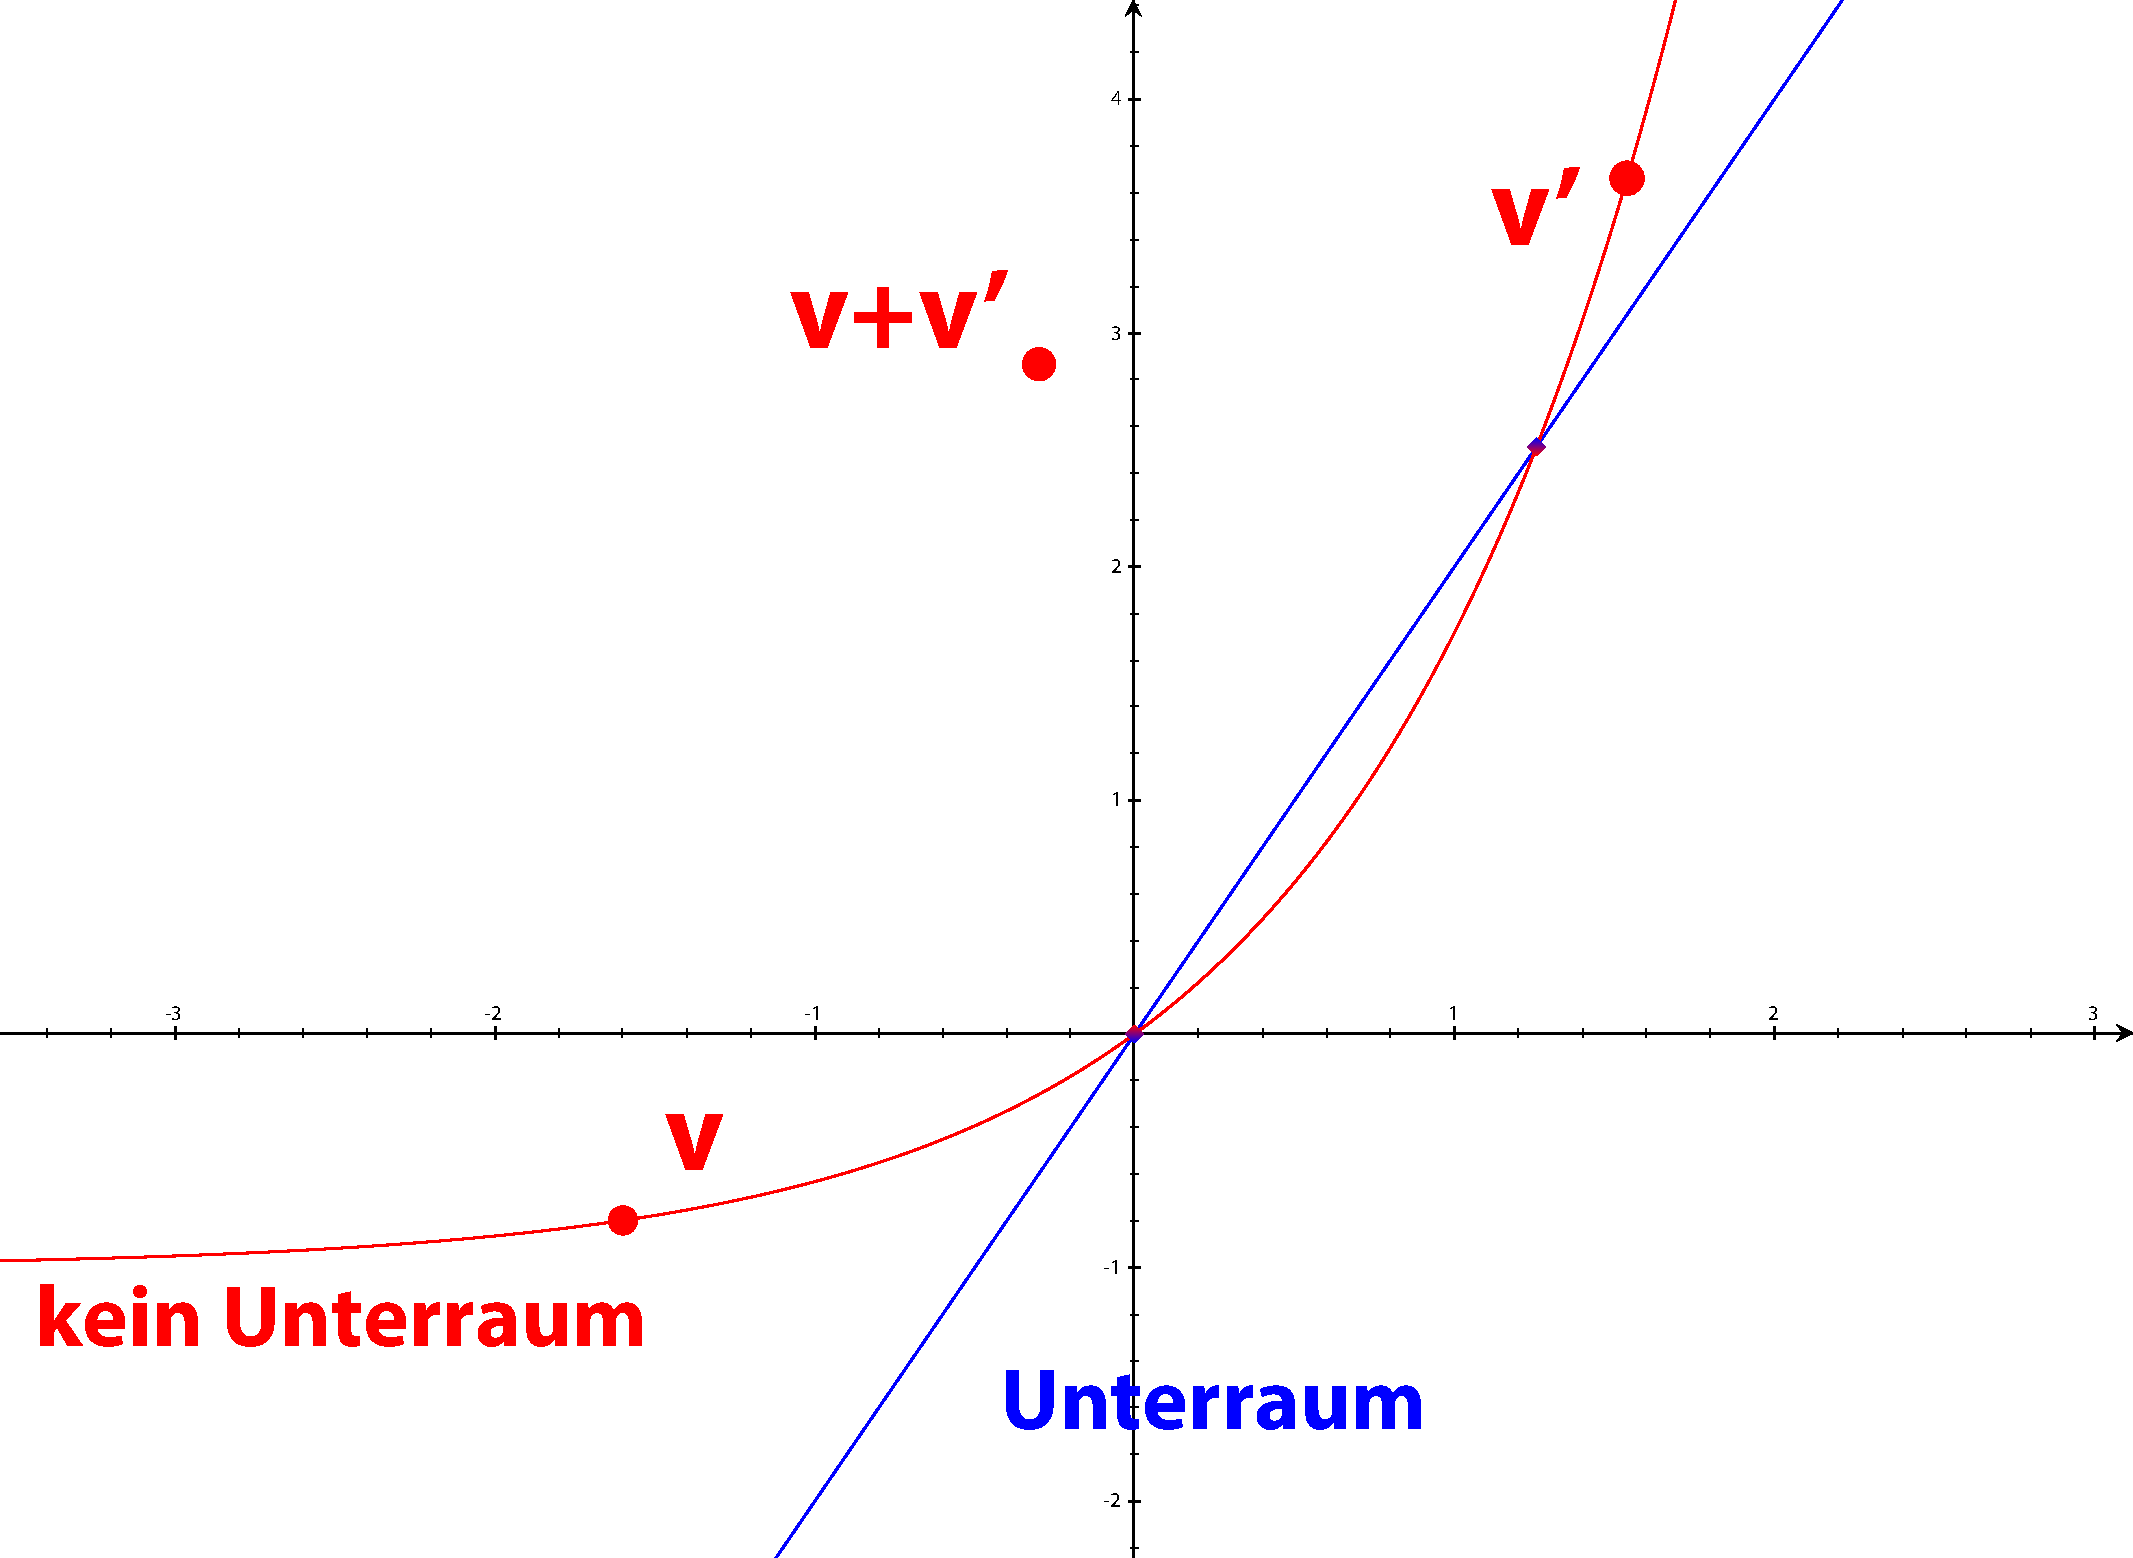
\includegraphics[scale=0.2]{veranschaulichung_untervektorraeume.pdf} \] \\
Es gibt in $ \mathds{R}^2 $ drei Klassen von Unterräumen:
\begin{itemize}[--]
	\item $U=\{ 0\}$ den Nullraum
	\item Geraden durch 0: für $a,b \in \mathds{R}$ \\
	$U = \bigg\{ \binom{x}{y} \mid ax +by = 0 \bigg\}$
	\item $U=\mathds{R}^2$
\end{itemize}
$\mathds{R}^3$ können wir als den 3-dimensionalen Raum veranschaulichen. \\
Es gibt in $\mathds{R}^3$ vier Arten von Unterräumen.
\begin{itemize} [--]
	\item $U=\{ 0 \}$
	\item Geraden durch 0 $U = \Bigg\{ \begin{pmatrix}
		x \\ y \\z
	\end{pmatrix} \mid \begin{matrix}
		ax +by +cz = 0 \\ \alpha x + \beta y + \gamma z  = 0
	\end{matrix}\Bigg\}$ für $a,b,c, \alpha, \beta, \gamma \in \mathds{R}$
	
	\item Ebenen, die 0 enthalten $U=  \Bigg\{ \begin{pmatrix}
		x \\ y \\z
	\end{pmatrix} \mid ax+by+cz \Bigg\}$ für $a,b,c \in \mathds{R}$
	\item $U=\mathds{R}^3$
\end{itemize}
% subsection beispiel (end)

\subsection{Beispiel} % (fold)
\label{sub:beispiel}
Seien $U_1$ und $U_2$ Unterräume eines $K$-Vektorraums $V$. Dann ist $U_1 \cup U_2$ nicht notwendig ein Unterraum.
Aber $U_1 + U_2 := \{v_1 + v_2 \mid v_1 \in U_1, v_2 \in U_2 \}$ ist ein ein Unterraum von $V$ \\
{\tiny (Man kann sich hier in Anlehnung an 3.11 zwei Geraden vorstellen)}
% subsection beispiel (end)
\subsection{Bemerkung} % (fold)
\label{sub:bemerkung}
Es gilt
\[
	(U_1 + U_2)+ U_3 = U_1 + (U_2 + U_3) = \{v_1 + v_2 + v_3 \mid v_1 \in U_1, v_2 \in U_2, v_3 \in U_3\}
\]
Allgemein schreiben wir für Unterräume $U_1, \ldots , U_n$ von $V$
\[
	U_1 + \ldots + U_n := \{ v_1 + v_2 + \ldots  + v_n \mid v_1 \in U_1, \ldots , v_n  \in U_n\}
\]
% subsection bemerkung (end)

\subsection{Satz} % (fold)
\label{sub:satz}
Seien $U_1, \ldots , U_n$ Unterräume des $K$-Vektorraums $V$ \\
Folgende Aussagen sind äquivalent:
\begin{enumerate}[(1)]
	\item Jeder Vektor $v \in V$ besitzt eine eindeutige Darstellung der Form 
	$v= v_1 + \ldots + v_n$ mit $v_i \in U_i$ für $i=1, \ldots , n$
	\item $V= U_1 + \ldots  + U_n$ und für jedes $j \in \{1, \ldots , n\}$ gilt 
	\[
		U_j \cap (U_1 + \ldots  + U_{j-1} +U_{j+1}+ \ldots + U_n) = \{ 0\}
	\]
\end{enumerate}
\underline{\textbf{Beweis:}} ``(1) $\Rightarrow$ (2)'': \\
Seien $U_1, \ldots , U_n$ Unterräume, dass (1) gilt. \\
Es folgt $V= U_1 + \ldots + U_n$ da sich jeder Vektor $v \in V$ schreiben lässt als
\[
	v= v_1 + \ldots + v_n \enspace \text{mit} \enspace v_i \in U_i \enspace \text{für} \enspace i=1, \ldots , n
\]
Sei $j \in \{ 1, \ldots , n\}$ fest. \\
Sei $v \in U_j \cap (U_1 + \ldots  + U_{j-1} +U_{j+1}+ \ldots + U_n)$ \\
\vspace{\baselineskip} \\
Wir müssen zeigen: $v=0$ \\
Da $v \in  (U_1 + \ldots  + U_{j-1} +U_{j+1}+ \ldots + U_n)$ ist, gibt es 
\[
	v_i \in U_i \enspace \text{für} \enspace i=1, \ldots , j-1, j+1, \ldots , n
\] mit
\[
	\begin{array}{cccccccccccccl}
		v &= &v_1 &+ &\ldots &+ &v_{j-1} &+ &0 + &v_{j+1} &+ &\ldots &+ &v_n  \quad \text{Andererseits ist auch} \\
		v &= &0 &+ &\ldots &+ &0 &+ &v + &0 &+ &\ldots &+ &0 
	\end{array}
\]
Nach Vorraussetzung sind solche Darstellungen für $v$ eindeutig. Es folgt
\[
	v_1 = 0, \ldots , v_{j-1}=0 , 0=v , v_{j+1}=0, \ldots , v_n =0.
\]
Insbesondere ist $v=0$ \\

\newpage 
\underline{\textbf{Beweis:}} ``(1) $\Rightarrow$ (2)'' \\
Seien $U_1, \ldots , U_n$ Unterräume von $V$ für die (2) gilt. \\
Da $V=U_1 + \ldots + U_n$ lässt sich jeder Vektor $v \in V$ schreiben als
\[
	v = v_1 + \ldots  + v_n \enspace \text{mit} \enspace v_i \in U_i \enspace \text{für } \enspace i=1, \ldots , n
\]
Wir müssen noch zeigen, dass diese Darstellung eindeutig ist. \\
Seien also $v_1, V'_1 \in U_1, \ldots , v_n, v'_n \in U_n $ mit
\[
	( \star) \enspace \begin{matrix}
		v & = & v_1 & + \ldots + &  v_n \\
		v' & = & v'_1 & + \ldots  + & v'_n
	\end{matrix}
\]
Wir müssen noch zeigen 
\[
	v_j = v'_j \enspace \text{für alle } \enspace j \in \{ 1, \ldots  , n\}
\]
Sei $j \in \{1, \ldots , n \}$ fest \\
\[
	(\star) \Rightarrow \underbrace{v_j - v'_j}_{\in U_j} = \underbrace{\underbrace{(v_1 -v'_1)}_{\in U_1} + \ldots + 
	\underbrace{(v_{j-1}- v'_{j-1})}_{\in U_{j-1}} + \underbrace{(v_{j+1}- v'_{j+1})}_{\in U_{j+1}} + \ldots +
	\underbrace{(v_n - v'_n)}_{\in U_n}}_{ \in (U_1 + \ldots + U_{j-1} + U_{j+1} + \ldots + U_n) 
	}
\]
Also 
\[
	v'_j -v_j \in U_j \cap (U_1 + \ldots + U_{j-1} + U_{j+1} + \ldots  + U_n) = \{ 0 \}
\]
$\Rightarrow v'_j -v_j = 0$ \\
$\Rightarrow v'_j = v_j \quad \quad \quad \quad \Box$ \\ 
%\raggedleft{$\Box$}
% subsection satz (end)
\subsection{Definition} % (fold)
\label{sub:definition}
Sei $U$ ein Unterraum des $K$-Vektorraumes $V$.\\
Ein Unterraum $U'$ von $V$ heißt ein \underline{\textbf{Komplement}} zu $U$ falls $V = U +U'$ und $U \cap U' = \{0\}$.
% subsection definition (end)

\subsection{Bemerkung} % (fold)
\label{sub:bemerkung}
Ist $U'$ ein Komplement zu $U$, so ist auch $U$ ein Komplement zu $U'$. Wir schreiben dann auch $V= U \oplus U'$
% subsection bemerkung (end)

\subsection{Frage} % (fold)
\label{sub:frage}
Gibt es zu jedem Unterraum ein Komplement? 
% subsection frage (end)

\subsection{Beispiel} % (fold)
\label{sub:beispiel}
Seien $V$ und $W$ $K$-Vektorräume. \\
Dann wird das karthesische Produkt $V \times W$ zu einem $K$-Vektorraum durch 
\begin{align*}
	(v,w) + (v',w') &:= (v + v' , w+ w') \\
	\lambda (v,w) &:= (\lambda v , \lambda  w)
\end{align*}
zu einem $K$-Vektorraum. Wir schreiben $V \oplus W$ für diesen Vektorraum. Er besitzt Unterräume $V \times \{0\} , \{0\} \times W$ und es gilt 
\[
	V \oplus W = (V \times \{0\}) \oplus (\{0\} \times W) 
\]
Beispiel: $K^n = \underbrace{K \oplus \ldots \oplus K}_{\text{$n$-mal}}$
% subsection beispiel (end)

\section{Basis und Dimension} % (fold)
\label{sec:basis_und_dimension}

\subsection{Definition} % (fold)
\label{sub:definition}
Sei $S$ eine Teilmenge des $K$-Vektorraum $V$. Der Durchschnitt aller Unterräume von $V$, die $S$ enthalten
\[
	\mathcal{L}(S) := \bigcap_{S \subseteq U} U
\]
heißt die \underline{\textbf{lineare Hülle}} von $S$ 
\vspace{\baselineskip} \\
Gilt $\mathcal{L}(S) = V$ so sagen wir $S$ \underline{\textbf{erzeugt}} $V$ oder $S$ ist ein \underline{\textbf{Erzeugendensystem}} (EZS) von $V$
% subsection definition (end)

\subsection{Beispiel} % (fold)
\label{sub:beispiel}
\[
	\mathcal{L}(\emptyset) = \{ 0 \}
\]
% subsection beispiel (end)

\subsection{Bemerkung} % (fold)
\label{sub:bemerkung}
\[
	\mathcal{L} (S) = \{ \lambda_1 v_1  + \ldots  + \lambda_n v_n \mid n \in \mathds{N} , v_1, \ldots  v_n \in S , \lambda_1, \ldots , \lambda_n \in K\}
\]
% subsection bemerkung (end)

\subsection{Definition} % (fold)
\label{sub:definition}
Für $v_1, \ldots , v_n \in V , \lambda_1, \ldots , \lambda_n \in K$ heißt $\lambda_1 v_1 + \ldots + \lambda_n v_n$ ein \underline{\textbf{Linearkombination}}
von $v_1, \ldots , v_n$. Falls mindestens ein $\lambda_i \not= 0$ ist, so heißt die Linearkombination \underline{\textbf{nicht trivial}}.
% subsection definition (end)

\subsection{Beispiel} % (fold)
\label{sub:beispiel}
Sei 
\[
	e_i = \begin{pmatrix} 0 \\ : \\ 1 \\ : \\ 0 \end{pmatrix} \in K^n \text{ für } i=1, \ldots , n
\]
Dann ist 
\[
	\begin{pmatrix} \lambda_1 \\ : \\ \lambda_n \end{pmatrix} = \lambda_1 e_1 + \ldots + \lambda_n e_n
\] 
Also ist $ \{ e_1, \ldots , e_n\}$ ein EZS für $K^n$
% subsection beispiel (end)

\subsection{Beispiel} % (fold)
\label{sub:beispiel}
Jeder Vektorraum $V$ besitzt ein EZS $S=V$. Dann ist $\mathcal{L} (S) = V$
% subsection beispiel (end)
\subsection{Frage} % (fold)
\label{sub:frage}
Besitzt jeder Vektorraum ein endliches Erzeugungssystem?
% subsection frage (end)

\subsection{Beispiel} % (fold)
\label{sub:beispiel}
Sind $U_1, \ldots  , U_n$ Unterräume von $V$, so gilt
\[
	\mathcal{L} (U_1 \cup \ldots \cup U_n) = U_1 + \ldots  + U_n
\]
% subsection beispiel (end)

\subsection{Beispiel} % (fold)
\label{sub:beispiel}
Betrachte das homogene Gleichungssystem über $\mathds{R}$:
\[
	\begin{array}{lccllll}
	x_1 & + & x_2 & + & x_3 & = & 0 \\
	x_1 & + & 2 x_2  & + & 3 x_3 &  =  & 0 \\
\end{array}
\]
äquivalent zu:
\[
	\begin{array}{lccllll}
	x_1 & + & x_2 & + & x_3 & = & 0 \\
	 &  & x_2  & + & 2 x_3 &  =  & 0 \\
\end{array}
\]
Der Lösungsraum ist \[
	= \Bigg\{ \begin{pmatrix} \lambda \\ -2 \lambda \\ \lambda \end{pmatrix} \mid \lambda \in \mathds{R} \Bigg\} 
= \mathcal{L} \Bigg( \begin{pmatrix}1 \\ -2 \\ 1  \end{pmatrix} \Bigg)
\]
Also ist $ \Bigg\{ \begin{pmatrix}1 \\ -2 \\1 \end{pmatrix} \Bigg\}$ ein EZS für $L$
% subsection beispiel (end)

\subsection{Definition} % (fold)
\label{sub:definition}
Sei $V$ ein $K$-Vektorraum und $S \leq V$. Die Menge $S$ heißt \underline{\textbf{linear unabhängig}}, falls für jedes $v \in S$ gilt:
\[
	v \not\in \mathcal{L} (S \backslash \{v\})
\]
Anderfalls heißt $S$ \textbf{\underline{linear abhängig}}.
% subsection definition (end)

\subsection{Lemma} % (fold)
\label{sub:Lemma}
Sei $V$ ein $K$-Vektorraum und $S= \{ v_1, \ldots , v_n\} \subseteq V$, wobei $v_i \not= v_j$ für $i \not= j$. \\
Dann ist $S= \{ v_1, \ldots  , v_n\}$ genau dann linear unabhängig, wenn gilt
\[
	(\star) \quad \text{ Ist } \lambda_1 v_1 + \ldots  + \lambda_n v_n = 0 \text{ mit } \lambda_1, \ldots , \lambda_n \in K \text{, so folgt } \lambda_1 = \ldots = \lambda_n = 0
\]
% subsection Lemma (end)

\subsection{Bemerkung} % (fold)
\label{sub:bemerkung}
Für $(\star)$ sagen wir auch, $\{v_1, \ldots , v_n\}$ erfüllt keine nicht triviale lineare Relation. \\
\vspace{\baselineskip} \\
\underline{\textbf{Beweis von 4.11}}
\vspace{\baselineskip} \\
\enquote{$\Longrightarrow$} \\
Sei $S$ linear unabhängig. Seien $\lambda_1, \ldots , \lambda_n \in K$ mit $\lambda_1 v_1 + \ldots + \lambda_n v_n = 0$ \\
\underline{Zu zeigen:}
\[
	\lambda_1 = \lambda_2 = \ldots = \lambda_n = 0
\]
Angenommen $\lambda_i \not= 0$, dann folgt
\[
	v_i = - (\lambda_1^{-1}) \big(\lambda_1 v_1+ \ldots + \lambda_{i-1} v_{i-1} + \lambda_{i+1} v_{i+1} + \ldots + \lambda_n v_n \big)
	\in \mathcal{L} (S \backslash \{v\})
\]
im Widerspruch zur linearen Unabhängigkeit von $S$. Also $\lambda_i = 0$ \\
\vspace{\baselineskip} \\
\enquote{$\Longleftarrow$} \\
erfülle $S$ nun keine nicht triviale lineare Relation. \\
Angenommen $S$ wäre linear abhängig. 
\vspace{\baselineskip} \\
Dann gibt es $v  \in \{1, \ldots , n\}$ mit $v_i \in \mathcal{L}(S \backslash \{v_i\})$. Also ist $v_i$ eine Linearkombination von $v_1, \ldots , v_{i-1}, v_{i+1}, \ldots , v_n$. Es gilt also
$\lambda_1, \ldots , \lambda_{i-1}, \lambda_{i+1}, \ldots , \lambda_n \in K$ mit 
\[
	v_i = \lambda_1 v_1 + \ldots + \lambda_{i-1} v_{i-1} + \lambda_{i+1} v_{i+1} + \ldots + \lambda_n v_n
\]
Es folgt \[
	0= \lambda_1 v_1 + \ldots + \lambda_{i-1} v_{i-1} + \lambda_{i+1} - v_i +v_{i+1} + \ldots + \lambda_n v_n
\]
Dies ist eine nicht triviale lineare Relation {\huge $\lightning$}
% subsection bemerkung (end)

\subsection{Beispiele} % (fold)
\label{sub:beispiele}
\begin{enumerate}[(i)]
	\item $\{ e_1, \ldots , e_n\} \subseteq K^n$ aus 4.5 ist linear unabhängig
	\item $ \Bigg\{ \begin{pmatrix} 1 \\ 2 \\ 3 \end{pmatrix}, \begin{pmatrix} 0 \\ 1 \\ 2 \end{pmatrix}, \begin{pmatrix} 0 \\ 0 \\ 1
	 \end{pmatrix} \Bigg\} \subseteq \mathds{R}^3 $ ist linear unabhängig
	 \item $ \Bigg\{ \begin{pmatrix} 1 \\ 2 \\ 3 \end{pmatrix}, \begin{pmatrix} 0 \\ 1 \\ 2 \end{pmatrix}, \begin{pmatrix} 2 \\ 3 \\ 4
	 \end{pmatrix} \Bigg\} \subseteq \mathds{R}^3 $ ist linear abhängig
	 \item Ist $0 \in S$, so ist $S$ linear abhängig
	 \item $\{v\}$ ist linear unabhängig $\Leftrightarrow v \not= 0$
\end{enumerate}
% subsection beispiele (end)

\subsection{Bemerkung} % (fold)
\label{sub:bemerkung}
Eine Folge $v_1, \ldots , v_n$ von Vektoren heißt linear unabhängig, wenn sie aus paarweise verschiedenen Vektoren besteht und die Menge
$\{ v_1, \ldots  , v_n \}$ linear unabhängig ist. Dies ist äquivalent dazu, dass $v_1, \ldots , v_n$ keine nicht triviale lineare Relation erfüllen. \\
Ist
\[
	\lambda_1 v_1 + \ldots + \lambda_n v_n = 0 \text{ mit } \lambda_1, \ldots , \lambda_n \in K
\]
so gilt:
\[
	\lambda_1 = \lambda_2 = \ldots = \lambda_n = 0
\]
% subsection bemerkung (end)

\subsection{Definition} % (fold)
\label{sub:definition}
Eine Teilmenge $B$ eines Vektorraumes $V$ heißt eine \underline{\textbf{Basis}}, wenn $B$ linear unabhängig ist und $V$ erzeugt.
% subsection definition (end)

\subsection{Bespiel} % (fold)
\label{sub:bespiel}
$\{ e_1, \ldots , e_n \subseteq K^n\}$ aus 4.5 ist eine Basis von $K^n$ und heißt \underline{\textbf{Standardbasis}} des $K^n$. $e_i$ heißt der der $i$-te \underline{\textbf{Standardvektor}} des $K^n$.
% subsection bespiel (end)

\subsection{Basisergänzungssatz} % (fold)
\label{sub:basisergänzungssatz}
Sei $V$ ein $K$-Vektorraum. Seien $M \subseteq S \subseteq V$, wobei $S$ ein EZS von $V$ sei und $M$ linear unabhängig sei. \\
Dann gibt es eine Basis $B$ mit $M \subseteq B \subseteq S$. Insbesondere besitzt jeder Vektorraum eine Basis. \\
\vspace{\baselineskip} \\
\underline{\textbf{Beweis:}} (für den Fall, dass $S$ endlich ist) \\
Unter allen linear unabhängigen Teilmengen $X$ von $V$ mit $M \subseteq X \subseteq S$ wählen wir ein maximales $X$ aus, etwa
\[
	B = \left\{ b_1, \ldots , b_n \right\}
\]
Es genügt nun $\mathcal{L}(B) = V$ zu zeigen. Dazu genügt es $S \subseteq \mathcal{L}(B)$ zu zeigen: 
\vspace{\baselineskip} \\
Sei $x \in S$. Ist $x \in B$ so folgt  $x \in \mathcal{L}(B)$. Andernfalls ist $B \cup \{x\}$ linear abhängig. Daher  
(Lemma 4.11 + 2.12) gibt es eine nicht triviale lineare Relation
\[
	\mu x + \lambda_1 b_1 + \ldots + \lambda_n b_n =0 
	\quad \text{mit } \mu, \lambda_1, \ldots , \lambda_n \in K \text{ und nicht alle 0}
\]
Wäre $\mu =0$, so wären auch $\lambda_1, \ldots , \lambda_n = 0$ , da $b_1, \ldots , b_n$ linear unabhängig ist. \\
Also $\mu \not= 0$
\[
	x = \mu^{-1} (- \lambda _1 b_1 - \ldots - \lambda_n b_n) \in \mathcal{L} (B)
\]
% subsection basisergänzungssatz (end)

\subsection{Bemerkung} % (fold)
\label{sub:bemerkung}
Für ein unendliches $S$ funktioniert der Beweis unter Benutzung des \textbf{Zorn'schen Lemmas} aus der Mengenlehre genauso.
% subsection bemerkung (end)

\subsection{Definition} % (fold)
\label{sub:definition}
Sei $X$ eine endliche Menge. Die Anzahl der Elemente von $X$ nennen wir die \underline{\textbf{Mächtigkeit}} von $X$. Wir schreiben auch $|X|$ für die Mächtigkeit von $X$. 
\vspace{\baselineskip} \\
Bsp: $\left| \{0,1, \ldots , n\} \right| =n+1$
% subsection definition (end)

\subsection{Dimensionssatz} % (fold)
\label{sub:dimensionssatz}
Sei $V$ ein $K$-Vektorraum, der ein endliches EZS $S$ besitzt. Dann haben je zwei Basen dieselbe Mächtigkeit.
% subsection dimensionssatz (end)

\subsection{Austauschsatz von Steinitz} % (fold)
\label{sub:dimensionssatz}
Sei $V$ ein $K$-Vektorraum. Sei $S$ eine endliche linear unabhängige Menge in $V$ und $T$ ein endliches Erzeugendensystem von $V$. \\
Dann gilt $|S| \leq |T|$ und $S$ lässt sich durch $|T| - |S|$ Elemente von $T$ zu einem Erzeugendensystem ergänzen.
% subsection dimensionssatz (end)

\subsection{Definition} % (fold)
\label{sub:definition}
Sei $V$ ein $K$-Vektorraum. Die \underline{\textbf{Dimension}} von $V$ über $K$ ist die Mächtigkeit einer (und damit jeder) Basis von $V$. \\
Wir schreiben auch $\dim_K V$ für die Dimension.
% subsection definition (end)

\subsection{Bemerkung} % (fold)
\label{sub:bemerkung}
Gibt es kein endliches EZS für $V$, so gilt
$\dim_K V = \infty$

% subsection bemerkung (end)

\subsection{Beispiel} % (fold)
\label{sub:beispiel}
$\dim K^n = n$
\newpage
{\large \underline{\textbf{Beweis des Austauschsatzes}}}
\vspace{\baselineskip} \\
Durch Induktion über die Mächtigkeit $|S|$ von $S$
\vspace{\baselineskip} \\
\textbf{Induktionsanfang:} \\
Sei $|S|=0$, dann ist $S = \emptyset$ \\
Dann können wir $S$ durch alle (also $|T|= |T| -|S|$ viele) Elemente von $T$ zu einem EZS ergänzen.
\vspace{\baselineskip} \\
\textbf{Induktionsschritt:} \\
Sei $|S| = n \geq 1$. Sei $b \in S$ und $S' = S \backslash \{b\}$ \\
Dann $|S'| = n-1$. Wir können also die Induktionsannahme auf $S'$ anwenden und finden $T' \subseteq T$ mit $|T'| = |T| - |S'|$
so dass $S' \cup T'$ ein EZS für $V$ ist.
\vspace{\baselineskip} \\
Nun lässt sich $b$ als Linearkombination der Elemente von $S' \cup T'$ schreiben:
\[
	b= \sum_{x \in S' \cup T'} \lambda_x \cdot x \quad \text{mit } \lambda_x \in K
\]
Behauptung ($\star$):
\[
	(\star) \quad \exists x_0 \in T' \text{ mit } \lambda_{x_0} \not= 0
\]
Angenommen dies gilt nicht, dann $\lambda_{x_0} = 0$ für alle $x \in T'$. Dann
\[
	b = \sum_{x \in S'} \lambda_x \cdot x
\]
im Widerspruch zur linearen Unabhängigkeit von $S= S' \cup \{ b\}$ {\huge $\lightning$}
\vspace{\baselineskip} \\
Mit ($\star$) folgt:
\[
	x_0 = (\lambda_{x_0})^{-1} \left( b - \sum_{x \in S' \cup (T' \backslash \{ x_0 \})} \lambda_{x} x \right) \in \mathcal{L} (S \cup T_0)
\]
Sei $T_0 = T' \backslash \{ x_0\}$ \\
Es folgt
\[
	\mathcal{L} (S \cup T_0) = \mathcal{L} \underset{\supseteq S' \cup T'}{(S \cup T')} = V
\]
Also ist $S \cup T_0$ ein EZS.
\vspace{\baselineskip} \\
Weiter ist 
\[
	|T_0| = |T'| -1 = |T| - |S'| -1 = |T| - \underbrace{(|S'| +1)}_{ |S|} = |T| - |S| \qquad \Box
\]
\newpage
{\large \underline{\textbf{Beweis des Dimensionssatzes}}}
Seien $B$ und $B'$ endliche Basen von $V$. Mit dem Austauschsatz für $S=B$ und $T=B'$ folgt
\[
	|B| = |S| \leq |T| = |B'|
\]
umgekehrt folgt auch $|B'| \leq |B|$. Also $|B| = |B'|$
% subsection beispiel (end)

\subsection{Korollar} % (fold)
\label{sub:korollar}
Sei $V$ ein $n$-dimensionaler $K$-Vektorraum und $S \subseteq V$ eine Teilmenge mit $|S| =n$. Dann gilt
\begin{enumerate}[(i)]
	\item Ist $S$ linear unabhängig, so ist $S$ eine Basis
	\item Ist $S$ ein EZS, so ist $S$ eine Basis
\end{enumerate}
\textbf{Beweis:} 
\begin{enumerate}[(i)]
	\item Nach dem Basisergänzungssatz lässt sich $S$ zu einer Basis $B$ ergänzen. Nach dem Dimensionssatz gilt $|B|=n$. 
	Da $S \subseteq B$ und $|S|=n$ folgt $S=B$. Damit ist $S$ eine Basis
	\item Nach dem Basisergänzungssatz finden wir eine Basis $B$ von $V$ mit $B \subseteq S$. Nach dem Dimensionssatz gilt
	$|B|=n$. Da $S \subseteq  B$ und $|S|=n$ folgt $S=B$. Damit ist $S$ eine Basis.
\end{enumerate}
% subsection korollar (end)

\subsection{Korollar} % (fold)
\label{sub:korollar}
Sei $U$ ein Unterraum des $K$-Vektorraums $V$. \\
Dann ist 
\[
	\dim_K U \leq \dim_K V
\]
Beweis: \\
Jede Basis $B_0$ von $U$ lässt sich nach dem Basisergänzungssatz zu einer Basis $B$ von $V$ ergänzen. Also 
\[
	\dim U = |B_0| \leq |B| = \dim V
\]
% subsection korollar (end)

\subsection{Beispiel} % (fold)
\label{sub:beispiel}
Sei $L$ der Lösungsraum des folgenden homogenen linearen Gleichungssystems über $\mathds{R}$
\[
\begin{array}{lllll}
x_1 &+ 2x_2 &+ 3x_3 &+ 4x_4 &= 0 \\
x_1 &- x_2 &+ x_3 &- x_4 &= 0 \\
4 x_1 &- x_2 &+ 6 x_3 &+ x_4 &= 0
\end{array}
\]
\[
	\begin{pmatrix}
	1 & 2 & 3 & 4 \\
	1 & -1 & 1 & -1 \\
	4 & -1 & 6 & 1 
	\end{pmatrix}
	\overset{\text{(II)}}{\leadsto}
	\begin{pmatrix}
	1 & -1 & 1 & -1 \\
	1 & 2 & 3 & 4 \\
	4 & -1 & 6 & 1 
	\end{pmatrix}
	\overset{\text{(I)}}{\leadsto}
	\begin{pmatrix}
	1 & -1 & 1 & -1 \\
	0 & 3 & 2 & 5 \\
	0 & 3 & 2 & 5 
	\end{pmatrix}
	\overset{\text{(I)}}{\leadsto}
	\begin{pmatrix}
	1 & -1 & 1 & -1 \\
	0 & 1 & \frac{2}{3} & \frac{5}{3} \\
	0 & 0 & 0 & 0 
	\end{pmatrix}
\]
Also:
\[
	L=
	\left\{
	\begin{pmatrix}
		x_1 \\ x_2 \\x_3
	\end{pmatrix}
	\Bigg| \enspace
	\begin{matrix}
		x_3 , x_4 \in \mathds{R} \\
		x_2 = - \frac{2}{3} x_3 -\frac{5}{3} x_4 \\
		x_1 = x_2 -x_3 +x_4 = - \frac{5}{3} x_3 - \frac{2}{3} x_4
	\end{matrix}
	\right\}
\]
oder:
\[
	L = \left\{
	\lambda 
	\begin{pmatrix}
		- \frac{2}{3} \\ - \frac{5}{3} \\ 0 \\ 1
	\end{pmatrix}
	+ \mu
	\begin{pmatrix}
		- \frac{5}{3} \\ - \frac{2}{3} \\ 1 \\ 0
	\end{pmatrix}
	\Bigg| \enspace
	\lambda , \mu  \in \mathds{R}
	\right\}
\]
Damit ist 
\[
	B = \left\{ 
	\begin{pmatrix}
		- \frac{2}{3} \\ - \frac{5}{3} \\ 0 \\ 1
	\end{pmatrix}
	,
	\begin{pmatrix}
		- \frac{5}{3} \\ - \frac{2}{3} \\ 1 \\ 0
	\end{pmatrix}
	\right\}
\]
eine Basis von $L$ (da $B$ linear unabhängig) \\
Es folgt also:
\[
	\dim L = 2
\]
% subsection beispiel (end)

\subsection{Bemerkung} % (fold)
\label{sub:bemerkung}
Sei $B$ eine endliche Basis des \(K\)-Vektorraums $V$. \\
Schreibe 
\[
	B= \{ b_1, b_2, \ldots , b_n\} \quad (\text{mit } b_i \not= b_j \text{ für } i \not= j)
\]
Wir nennen das $n$-Tupel $(b_1, b_2, \ldots , b_n)$ von Vektoren eine \underline{\textbf{geordnete Basis}} von $V$. \\
Jeder Vektor $v \in V$ hat dann eine Darstellung als 
\[
	v= \lambda_1 b_1 + \lambda_2 b_2 + \ldots + \lambda_n b_n
\]
da $B$ ein EZS ist. Da $B$ auch linear unabhängig ist, sind alle $v$ durch $\lambda_i$ auch auch eindeutig dargestellt.
Denn aus
\begin{gather*}
	\lambda_1 b_1 + \lambda_2 b_2 + \ldots + \lambda_n b_n = \mu_1 b_1 + \mu_2 b_2 + \ldots + \mu_n b_n \\
	\Rightarrow \enspace (\lambda_1 - \mu_1)b_1 + (\lambda_2 - \mu_2)b_2 + \ldots + (\lambda_n \mu_n)b_n = 0
\end{gather*}
folgt
\[
	\lambda_1 = \mu_1 , \lambda_2 =\mu_2 , \ldots , \lambda_n = \mu_n
\]
da $B$ linear unabhängig
% subsection bemerkung (end)

\subsection{Bemerkung} % (fold)
\label{sub:bemerkung}
Die Beobachtung aus 4.28 lässt sich auch wie folgt formulieren:
\vspace{\baselineskip} \\
Sei $(b_1 , b_2, \ldots , b_n)$ eine geordnete Basis von $V$.
Definiere
\[
	\varphi_B : K^n \to V \quad \text{durch } \varphi_B 
	\begin{pmatrix}
		\lambda_1 \\ \vdots \\ \lambda_n
	\end{pmatrix}
	:= \lambda_1 b_1 + \lambda_2 b_2 + \ldots + \lambda_n b_n
\]
Dann ist $\varphi_B$ eine lineare Abbildung. Da $B$ ein EZS ist, ist $\varphi_B$ surjektiv. Da $B$ linear unabhängig ist, ist $\varphi_B$
injektiv. Also ist $\varphi_B$ bijektiv.
% subsection bemerkung (end)

\subsection{Satz} % (fold)
\label{sub:satz}
Sei $U$ ein Unterraum des \(K\)-Vektorraums $V$. Dann gibt es eine Komplement $W$ zu $U$, also einen Unterraum $W$ von $V$ mit 
$V=U \oplus W$ \\
\vspace{\baselineskip} \\
\underline{\textbf{Beweis:}} \\
Sei $B_0$ eine Basis von $U$. Nach dem Basisergänzungssatz können wir $B_0$ zu einer Basis von $V$ ergänzen. 
Sei $B_1 := B \backslash B_0$ und $W := \mathcal{L}(B_1)$ 
\vspace{\baselineskip} \\
\textbf{Behauptung:} $V= U \oplus W$ \\
zu zeigen:
\begin{enumerate}[(1)]
	\item $U \cap W = \{ 0\}$
	\item $U + W = V$
\end{enumerate}
\underline{zu(1):} \\
Sei $v \in U \cap W$. Da $v \in U$ gibt es $b_1 , \ldots , b_n \in B_0$ und $\lambda_1 , \ldots  , \lambda_n \in K$ mit 
$v= \sum\limits_{i=1}^{n} \lambda_i b_i$ \\
Da auch $v \in W$ gibt es $b'_1 , \ldots , b'_n \in B_1$ und $\mu_1 , \ldots ,\mu_n \in K$ mit 
$v = \sum\limits_{i=1}^n \mu_i b'_i$ \\
Es folgt:
\[
	\lambda_1 b_1 + \lambda_2 b_2 + \ldots + \lambda_n b_n - \mu_1 b'_1 - \mu_2 b'_2 - \ldots - \mu_n b'_n = 0
\]
Da $b_1, b_2, \ldots , b_n , b'_1, b'_2 , \ldots b'_n \subseteq B$ und somit linear unabhängig über $K$ ist, folgt:
\[
	\lambda_1 = \ldots = \lambda_n = \mu_1 = \ldots =\mu_n = 0
\]
Damit ist auch $v=0$ 
\vspace{\baselineskip} \\
\underline{zu(2):} \\
Es ist $V=\mathcal{L} (B)$ da $B$ Basis von $V$ ist. Es gilt weiter 
\[
	B=B_0 \cup B_1 \subseteq U \cup W \subseteq U +W =V
\]
Also $\mathcal{L}(B) \subseteq U +W$. Damit folgt $V \subseteq U +W$. Da auch $U + W \subseteq V$ gilt, folgt $U +W = V$ \quad $\Box$
% subsection satz (end)
% section basis_und_dimension (end)

\section{Die komplexen Zahlen} % (fold)
\label{sec:die_komplexen_zahlen}
\subsection{Konstruktion} % (fold)
\label{sub:konstruktion}
Betrachte den $\mathds{R}$-Vektorraum $\mathds{C} := \mathds{R}^2$. \\
Setze $1_{\mathds{C}} := \binom{1}{0}$ und $i_{\mathds{C}} := \binom{0}{1}$. Dann ist $ \{ 1_{\mathds{C}}, i_{\mathds{C}} \} $ 
eine $\mathds{R}$-Basis von $\mathds{C}$. \\
Jedes $ z \in \mathds{C}$ lässt sich eindeutig schreiben als $z= \alpha 1_{\mathds{C}} +\beta i_{\mathds{C}}$ mit 
$\alpha , \beta \in \mathds{R}$. Dabei heißt $\alpha = \text{Re} \, z$ der \underline{\textbf{Realteil}} von $z$ und 
$\beta = \text{Im} \, z$ der \underline{\textbf{Imaginärteil}} von $z$. Fast immer schreiben wir $1=1_{\mathds{C}}, i = i_{\mathds{C}}$
und $\alpha + \beta i = \alpha \cdot 1_{\mathds{C}} + \beta \cdot i_{\mathds{C}}$. 
\vspace{\baselineskip} \\
Das Produkt komplexer Zahlen $z= \alpha + \beta i$ und $z' = \alpha' + \beta' i$ wird definiert durch
\[
	z \cdot z' = (\alpha + \beta i)\cdot (\alpha' + \beta' i) := (\alpha \alpha' -\beta \beta') + (\alpha  \beta' + \beta \alpha') i
\]
Zu einer komplexen Zahl $z = \alpha + \beta i$ heißt $\bar z := \alpha - \beta i$ das Konjugierte zu $z$. Die Abbildung 
$\mathds{C} \to \mathds{C} , z \mapsto \bar z$ ist $\mathds{R}$-linear.
% subsection konstruktion (end)

\subsection{Bemerkung} % (fold)
\label{sub:bemerkung}
Merken muss man sich nur $i \cdot i = -1$. Alles andere ergibt sich aus den vertrauten Rechenregeln: 
\begin{align*}
	(\alpha  + \beta i) \cdot  (\alpha + \beta i) &= \alpha (\alpha' + \beta' i) + \beta i(\alpha' + \beta' i) \\
	&= \alpha \alpha' + \alpha \beta' i + \beta i \alpha' + \beta i \beta' i \\
	&= \alpha \alpha' + \alpha \beta' i + \beta \alpha' i + \beta \beta' i^2 \\
	&= \alpha \alpha' + \alpha \beta' i + \beta \alpha' i + \beta \beta' (-1) \\
	&= (\alpha \alpha' -\beta \beta') + (\alpha  \beta' + \beta \alpha') i
\end{align*}
% subsection bemerkung (end)

\subsection{Satz} % (fold)
\label{sub:satz}
Die komplexen Zahlen $\mathds{C}$ bilden einen Körper \\
\vspace{\baselineskip} \\
\underline{\textbf{Beweis:}} \\
Wir zeigen nur die Existenz eines multiplikativen Inversen und lassen alles andere als Übung. \\
Sei $z= \alpha + \beta i \in \mathds{C}$. Dann gilt
\[
	z \cdot \bar z = \alpha^2 + \beta^2
\]
Ist $z \not= 0$ so sind nicht $\alpha $ und $\beta$ Null. Insbesondere gibt es $\frac{1}{\alpha^2 + \beta^2} \in \mathds{R}$. 
Das mulitplikativ Inverse zu $z$ ist nun 
\[
	z^{-1} := \frac{1}{\alpha^2 + \beta^2} (\alpha -\beta i) = \frac{\alpha}{\alpha^2 + \beta^2} - \frac{\beta}{\alpha^2 + \beta^2} i
	\qquad \Box
\]
% subsection satz (end)

\subsection{Bemerkung} % (fold)
\label{sub:bemerkung}
Jede komplexe Zahl $z = \alpha + \beta i$ besitz eine Wurzel in $\mathds{C}$. (Übung!)
% subsection bemerkung (end)

\subsection{Fundamentalsatz der Algebra} % (fold)
\label{sub:fundamentalsatz_der_algebra}
Jedes nicht-konstante Polynom über $\mathds{C}$ besitzt eine Nullstelle in $\mathds{C}.$ \\
% subsection fundamentalsatz_der_algebra (end)
% section die_komplexen_zahlen (end)

\section{Lineare Abbildungen} % (fold)
\label{sec:lineare_abbildungen}

\subsection{Erinnerung} % (fold)
\label{sub:erinnerung}
Seien $V$ und $W$ $K$-Vektorräume. Eine Abbildung $f : V \to W$ heißt $K$-linear, falls gilt:
\begin{enumerate}[(i)]
	\item $\forall \lambda \in K \enspace \forall v \in V : f(\lambda v)= \lambda f(v)$
	\item $\forall v, v' \in V : f(v +v')= f(v) + f(v')$
\end{enumerate}
Die Menge aller $K$-linearen Abbildungen $V \to W$ bezeichnen wir mit $\hom_K (V,W)$
% subsection erinnerung (end)

\subsection{Beispiel} % (fold)
\label{sub:beispiel}
\begin{enumerate}[(i)]
	\item $f: \mathds{R}^3 \to \mathds{R}$ mit $f\left( \left(\begin{smallmatrix}x_1 \\ x_2 \\ x_3 \end{smallmatrix}
	\right) \right) = 3x_1 + 2x_2 + x_3$ ist linear
	\item $g: \mathds{R}^3 \to \mathds{R}$ mit $g\left( \left(\begin{smallmatrix}x_1 \\ x_2 \\ x_3 \end{smallmatrix}
	\right) \right) = 3x_1 + 2x_2 + x_3 + 4 $ ist nicht linear
	\item $h: \mathds{R}^3 \to \mathds{R}$ mit $h\left( \left(\begin{smallmatrix}x_1 \\ x_2 \\ x_3 \end{smallmatrix}
	\right) \right) = 3x_1 + 2x_2 + x_3^2$ ist nicht linear
	\item Sei $X$ eine Menge und $K^X$ der $K$-Vektorraum aller Abbildungen $F: X \to K$. Sei $x \in X$. Sei 
	$ev_x : K^X \to K $ mit $ev_x (f)= f(x)$. \\
	Dann ist $ev_x$ $K$-linear.
\end{enumerate}
% subsection beispiel (end)

\subsection{Bemerkung} % (fold)
\label{sub:bemerkung}
\begin{enumerate}[(i)]
	\item Seien $f: V \to W$ und $g: W \to U$ $K$-linear. Dann ist auch $g \circ f : V \to U$ $K$-linear
	\item Seien $f,g : V \to W$ $K$-linear. Dann ist auch $f+g: V \to W$ mit $(f+g)(v):=f(v)+g(v)$ $K$-linear
	\item Sei $f: V \to W$ \(K\)-linear und $\lambda \in K$. Dann ist auch $\lambda f : V \to W$ mit 
	$(\lambda \cdot f)(v):= \lambda \cdot  f(v)$ \(K\)-linear 
\end{enumerate}
% subsection bemerkung (end)

\subsection{Bemerkung} % (fold)
\label{sub:bemerkung}
$\hom_K (V,W)$ wird durch 6.3(ii) und (iii) ein \(K\)-Vektorraum.
% subsection bemerkung (end)

\subsection{Bemerkung} % (fold)
\label{sub:bemerkung}
Ist $f: V \to W$ \(K\)-linear, so gilt:
\begin{enumerate}[(i)]
	\item $f(0)=0$ denn $f(0)=f(0+0)= f(0)+f(0)$
	\item $f(-v)= - f(v)$
\end{enumerate}
% subsection bemerkung (end)

\subsection{Definition} % (fold)
\label{sub:definition}
Eine \(K\)-lineare Abbildung $f: V \to W$ heißt: 
\begin{itemize}
	\item \underline{\textbf{Epimorphismus}} falls $f$ surjektiv
	\item \underline{\textbf{Monomorphismus}} falls $f$ injektiv
	\item \underline{\textbf{Isomorphismus}} falls $f$ bijektiv
\end{itemize}
% subsection definition (end)

\subsection{Lemma} % (fold)
\label{sub:lemma}
Sei $f: V \to W$ ein Isomorphismus. \\
Dann ist die inverse Abbildung $f^{-1} : W \to V$ zu $f$ auch ein Isomorphismus, insbesondere \(K\)-linear.\\
\vspace{\baselineskip} \\
\textbf{Beweis:} \\
Bijektivität von $f^{-1}$ folgt aus der Bijektivität von $f$ 
\vspace{15 pt} \\
Zu $f^{-1}$ ist \(K\)-linear: \\
Die Abbildung $f^{-1} : W \to V$ wird charakterisiert durch die Gleichung 
\[
	f \big( f^{-1}(w) \big) =w
\]
für alle $w \in W$. \\
Seien $w,w'\in W$. Dann gilt:
\begin{align*}
	f \big( f^{-1} (w) + f^{-1} (w') \big) &= f \big(  f^{-1}(w) \big) + f \big( f^{-1} (w') \big) \\
	&= w +w'
\end{align*}
Also ist $f^{-1}(w) + f^{-1}(w') = f^{-1} (w + w')$. \\
Sei $w \in W, \lambda \in K$. Dann gilt:
\[
	f \big( \lambda \cdot f^{-1} (w) \big) = \lambda \cdot f \big( f^{-1} (w)\big) = \lambda \cdot w
\]
Also ist $f^{-1}(\lambda w) = \lambda  f^{-1}(w)$ \hfill $\square$
% subsection lemma (end)

\subsection{Bemerkung} % (fold)
\label{sub:bemerkung}
Sei $f: V \to W$ \(K\)-linear. \\
Dann ist $\bild (f) = \{ f(v) \mid v \in V \}$ ein Unterraum von $W$. 
Ebenso ist $ \text{Kern} (f) =  \{ v \in V \mid f(v) = 0 \} $ ein Unterraum von $V$.
\[
	\rg (f) := \dim \, \bild(f)
\]
heißt der \underline{\textbf{Rang}} von $f$
% subsection bemerkung (end)

\subsection{Beispiel} % (fold)
\label{sub:beispiel}
\begin{enumerate}[(i)]
	\item Sei $A=\left(
		\begin{smallmatrix}
			a_{11} & \cdots & a_{1n} \\
			\cdot  && \cdot \\
			a_{m1} & \cdots & a_{mn}
		\end{smallmatrix} \right)$
		eine $m \times n$-Matrix über $K$. \\
		{\small (Also $a_{ij} \in K$ für $i=1, \ldots  , m \enspace j=1, \ldots , n$)} \\
		Dann wird durch 
		\[
			f_A \left( \begin{smallmatrix} x_1 \\ \cdot \\x_n \end{smallmatrix} \right) := A x = \begin{pmatrix}
				\sum\limits_{j=1}^{n} a_{1j} x_j \\ : \\\sum\limits_{j=1}^{n} a_{mj} x_j
			\end{pmatrix} \in K^m
		\]
		eine lineare Abbildung $f_A : K^n \to K^m$ definiert. Es gilt dann:
		\begin{enumerate}[(1)]
			\item Kern$f$ ist der Raum der Lösungen des homogenen Gleichungssystems $Ax=0$
			\item $\bild f$ besteht genau aus den $b \in K^m$ für die das Gleichungssystem $Ax=b$ lösbar ist
		\end{enumerate}
	\item Sei $C$ eine $m \times n$-Matrix über $K$ der Form
	\[
		C= \begin{pmatrix}
			c_{11} & c_{12} & \cdots & \cdots & \cdots & c_{1n} \\
			0 & c_{22} & \cdots & \cdots & \cdots & c_{2n} \\
			\vdots & & \ddots & & & \vdots \\
			0 & \cdots & 0 & c_{rr} & \cdots & c_{rn} \\
			0 & \cdots & 0 & 0 & \cdots & 0 \\
			\vdots & & & & & \vdots \\
			0 & \cdots & 0 & 0 & \cdots & 0
		\end{pmatrix}
	\]
	mit $c_{11}, \ldots , c_{rr} \in K \backslash \{0\}$ 
	\vspace{\baselineskip} \\
	\textbf{Behauptung:} $\rg (f_C) = r$ \\
	\textbf{Beweis:}\\
	Sei $e_1, \ldots , e_n$ die Standardbasis des $K^n$. \\
	Sei $\hat e_1 , \ldots , \hat e_m$ die Standardbasis des $K^m$
	\vspace{\baselineskip} \\
	Es ist Bild$(f_C) \subseteq \mathcal{L} \big( \{ \hat e_1 , \ldots , \hat e_r \}\big)$. Daher ist $\rg (f_C) \leq r$ \\
	Es genügt zu zeigen $ \hat e_1 , \ldots , \hat e_r \in \text{Bild} (f_C)$. 
	Wir zeigen dies durch Induktion nach $k=1, \ldots , r$
	\vspace{\baselineskip} \\
	\textbf{I.A} :
	\[
		\hat e_1 = f_C (c_{11}^{-1} \cdot e_1) \in \text{Bild} (f_C)
	\]
	\textbf{I.S.} :
	\[
		< k \mapsto k
	\]
	Seien $\hat e_1 , \ldots , \hat e_{k-1} \in \text{Bild} (f_C)$. Es ist
	\[
		f_C (e_k) = c_{1k} \hat e_1 + \ldots + c_{kk} \hat e_{k}
	\]
	Also
	\[
		\hat e_k = c_{kk}^{-1} \Big( \underset{\in \text{Bild} f_C}{f_C (e_k)} - 
		\underset{\in \text{Bild} f_C}{c_{1k} \hat e_1} - \ldots - 
		\underset{\in \text{Bild} f_C}{c_{(k-1) k} \hat e_{k-1}} \Big) \in \text{Bild} f_C
	\]
\end{enumerate}
% subsection beispiel (end)

\subsection{Proposition} % (fold)
\label{sub:proposition}
Sei $f : V \to W$ \(K\)-linear. 
Dann ist $f$ genau dann injektiv, wenn gilt Kern$f =  \{ 0\}$ 
\vspace{\baselineskip} \\
\textbf{Beweis:} \\
\enquote{$\Rightarrow$} \\
Sei $f$ injektiv, sei $v \in \text{Kern}f$. Dann $f(v)=0 = f(0)$. Da $f$ injektiv, folgt $v=0$. Also Kern$f= \{ 0\}$
\vspace{\baselineskip} \\
\enquote{$\Leftarrow$} \\
Sei Kern$f = \{0\}$. Sei also $v,v' \in V$ mit $f(v)=f(v')$. \\
Dann $f(v-v')= f(v)-f(v')=0$ 
\vspace{9pt} \\
Also $v-v' \in \text{ Kern} f = \{0\}$. Also $v-v' =0$ \\
Daher $v=v'$. Somit ist $f$ injektiv \hfill $\square$
% subsection proposition (end)

\subsection{Bemerkung} % (fold)
\label{sub:bemerkung}
Sei $f : V \to W$ \(K\)-linear. Seien $x \in V , b \in W$ mit $f(x)=b$. Daher gilt:
\[
	\left\{ y \in V \mid f(y)=b \right\} =  \{ x +v \mid v \in \text{Kern} f \} =: x + \text{Kern} f
\]
\textbf{Beweis:} 
\vspace{\baselineskip} \\
\enquote{$\subseteq$} \\
Sei $y \in V$ mit $f(y)=b$. Dann 
\[
	f(y-x)= f(y)-f(x)= b-b=0
\]
Also $v=y-x \in \text{Kern} f$ und $y=x+v \in x + \text{Kern} f$
\vspace{\baselineskip} \\
\enquote{$\supseteq$} \\
Sei $v \in \text{Kern} f.$ Dann gilt
\[
	f(x+v)= f(x) +f(v) =b
\]
Also ist 
\[
	x+v \in \{ y \in V \mid f(y)=b  \} 
\]
\hfill $\square$
% subsection bemerkung (end)

\subsection{Satz} % (fold)
\label{sub:satz}
Sei $f: V \to W$ linear. Sei $b_1, \ldots , b_n$ eine Basis von Kern$f$. Seien $a_1, \ldots , a_m \in V$ sodass 
$f(a_1), \ldots , f(a_m)$ eine Basis von $\bild f$ ist. \\
Dann ist $b_1, \ldots , b_n , a_1, \ldots , a_m$ eine Basis von V.
\vspace{\baselineskip} \\
\underline{\textbf{Beweis:}} \\
Sei $v \in V$. Da $f(a_1), \ldots , f(a_m)$ Basis von Bild$f$, gibt es $\lambda_1 , \ldots , \lambda_m$ mit 
\[
	f(v)= \sum\limits_{i=1}^{m} \lambda_i f(a_i) = f \left(\sum\limits_{i=1}^{m} \lambda_i a_i\right)
\]
Es folgt
\[
	v - \sum\limits_{i=1}^{m} \lambda_i a_i \in \text{Kern}f
\]
Da $b_1 , \ldots , b_n$ Basis von Kern$f$ ist, gibt es $\mu_1, \ldots , \mu_n \in K$ mit
\[
	v- \sum\limits_{i=1}^{m} \lambda_i a_i = \sum\limits_{j=1}^{n} \mu_j b_j
\]
Also
\[
	v= \sum\limits_{j=1}^{n} \mu_j b_j + \sum\limits_{i=1}^{m} \lambda_i a_i
\]
Damit ist $b_1, \ldots , b_n, a_1, \ldots , a_m$ ein EZS. 
\vspace{\baselineskip} \\
Es bleibt zu zeigen $b_1, \ldots , b_n, a_1, \ldots , a_m$ ist linear unabhängig \\
Seien $\lambda_1 , \ldots , \lambda_m \in K$ und $\mu_1 , \ldots , \mu_n \in K$ mit
\[
	\mu_1 b_1 + \ldots + \mu_n b_n + \lambda_1 a_1 + \ldots + \lambda_m a_m =0
\]
Es folgt:
\[
	\lambda_1 f(a_1) + \ldots + \lambda_m f(a_m) =0
\]
$\xrightarrow{f(a_1), \ldots , f(a_m) \text{ ist l.u.}} \lambda_1 = \lambda_2 = \ldots = \lambda_m =0$ 
\vspace{8pt} \\
$\Longrightarrow \mu_1 b_1 + \ldots + \mu_n b_n =0$ 
\vspace{8pt} \\
$\xrightarrow{b_1, \ldots , b_n \text{ ist l.u.}} \mu_1 = \mu_2 = \ldots = \mu_n =0$
\vspace{8pt} \\
Damit ist auch $b_1, \ldots , b_n, a_1 , \ldots , a_m$ linear unabhängig \hfill $\square$
% subsection satz (end)

\subsection{Dimensionsformel} % (fold)
\label{sub:dimensionsformel}
Sei $f : V \to W$ linear, wobei $\dim V < \infty$. Dann gilt
\[
	\boxed{\dim \text{Kern}f + \dim \text{Bild}f = \dim V}
\]
Beweis folgt aus 6.12
% subsection dimensionsformel (end)

\subsection{Korollar} % (fold)
\label{sub:korollar}
Sei $f : V \to W$ linear, wobei $\dim V = \dim W < \infty$. Dann sind äquivalent:
\begin{enumerate}[(1)]
	\item Kern$f = \{0\}$
	\item Bild$f = W$
	\item $f$ ist bijektiv
\end{enumerate}
\textbf{Beweis:}
\begin{itemize}
	\item $(1) \Rightarrow (2)$ \\
	Sei Kern$f = \{0\}$ \\
	$\xrightarrow{\text{Dimensionsformel}} \underbrace{\dim \, \overbrace{\text{Kern}f}^{\{0\}}}_{0} + \dim \text{Bild}f = \dim 	V$ \\
	Also $\dim \text{Bild}f = \dim V < \infty$. Da aus Bild$f \subseteq W$ folgt Bild$f =W$ 
	\item $(2)\Rightarrow (3)$ \\
	Sei Bild$f =W$. Dann ist $f$ surjektiv. Mit der Dimensionsformel folgt 
	\begin{align*}
		\dim \text{Kern}f &= \dim V - \dim \bild f \\
		&= \dim V - \dim W \\
		&= 0
	\end{align*}
	Damit ist Kern$f = \{0\}$. Mit 6.10 folgt die Injektivität von $f$. Also ist $f$ bijektiv.
	\item $(3) \Rightarrow (1)$ \\
	$f$ bijektiv $\Rightarrow f$ injektiv $\overset{6.10}{\Rightarrow}$ Kern$f = \{0\}$
\end{itemize}
% subsection korollar (end)

\subsection{Bemerkung} % (fold)
\label{sub:bemerkung}
Sei $A$ eine $m \times n$-Matrix über $K$. Sei $f_A : K^n \to K^m , f_A (x) = A \cdot x$. Dann gelten
\begin{enumerate}[(i)]
	\item $f$ injektiv $\Rightarrow n \leq m$
	\item $f$ surjektiv $\Rightarrow n \geq m$
	\item $f$ bijektiv $\Rightarrow n =m$
\end{enumerate}
{\small ($n =$ \#Variablen , $m = $ \#Gleichungen)}
% subsection bemerkung (end)

\subsection{Lemma} % (fold)
\label{sub:lemma}
Sei $b_1, \ldots , b_n$ eine Basis von $V$ und $w_1 , \ldots , w_n \in W$. Dann gibt es genau eine lineare Abbildung $f: V \to W$
mit $f(b_i)=w_i$ für $i= 1, \ldots ,n$ \\
\newpage 
\underline{\textbf{Beweis:}}
\vspace{10pt} \\
\underline{Existenz von $f$} \\
Zu $v \in V$ gibt es eindeutige $\lambda_1 , \ldots , \lambda_n \in K$ mit $v= \lambda_1 b_1 + \ldots + \lambda_n b_n$. Setze:
\[
	f(v)= \lambda_1 w_1 +\ldots + \lambda_n w_n = \sum\limits_{i=1}^{n} \lambda_i w_i
\]
\underline{$f$ ist linear}
\begin{enumerate}[(i)]
	\item Sei $\lambda \in K$ und $v= \sum\limits_{i=1}^{n} \lambda_i b_i \in V$. Dann ist 
	\[
		\lambda v = \lambda \cdot \sum\limits_{i=1}^{n} \lambda_i b_i = \sum\limits_{i=1}^{n} (\lambda \lambda_i) b_i
	\]
	Also
	\[
		f(\lambda v)= \sum\limits_{i=1}^{n} (\lambda \lambda_i) w_i = \lambda \sum\limits_{i=1}^{n} \lambda_i w_i = \lambda \cdot f(v)
	\]
	\item Seien $v= \sum\limits_{i=1}^{n} \lambda_i b_i \enspace, \enspace v' = \sum\limits_{i=1}^{n} \lambda'_i b_i \in V$. Dann
	\[
		v+v' = \sum\limits_{i=1}^{n} \lambda_i b_i + \sum\limits_{i=1}^{n} \lambda'_i b_i = \sum\limits_{i=1}^{n} (\lambda_i +\lambda'_i) b_i
	\]
	Also
	\[
		f(v+v') \sum\limits_{i=1}^{n} (\lambda_i +\lambda'_i) w_i = \sum\limits_{i=1}^{n} \lambda_i w_i + \sum\limits_{i=1}^{n} \lambda'_i w_i
		= f(v)+ f(v')
	\]
\end{enumerate}
\underline{Eindeutigkeit von $f$} \\
Sei $g: V \to W$ eine zweite lineare Abbildung mit $g(b_i)= w$ für $i=1, \ldots , n$. \\
Sei $v= \sum\limits_{i=1}^{n} \lambda_i b_i \in V$. Dann
\[
	f(v)= f \left(\sum\limits_{i=1}^{n} \lambda_i b_i\right) = \sum\limits_{i=1}^{n} \lambda_i f(b_i) = \sum\limits_{i=1}^{n} \lambda_i g(b_i) 
	= g \left(\sum\limits_{i=1}^{n} \lambda_i b_i \right) = g(v)
\]
\hfill $\square$
% subsection lemma (end)

\subsection{Satz} % (fold)
\label{sub:satz}
Seien $V,W$ \(K\)-Vektorräume mit $\dim V < \infty$ und $\dim W < \infty$. Dann sind äquivalent
\begin{enumerate}[(1)]
	\item Es gibt einen Isomorphismus $f: V \to W$
	\item $\dim V = \dim W$
\end{enumerate}
\underline{\textbf{Beweis:}} $(1) \Rightarrow (2)$ \\
Sei $f: V \to W$ linear und bijektiv. Dann Kern$f = \{0\}$ und Bild$f = W$ \\
Mit der Dimensionsformel folgt
\[
	\dim W = \dim \bild f \underset{\text{Dim.Formel}}{\underset{\uparrow}{=}} \dim V - \dim \text{ Kern} f = \dim V
\]
$(2) \Rightarrow (1)$ \\
Sei $\dim V = \dim W = n$. Wähle Basen $b_1, \ldots , b_n$ von $V$ und $a_1 , \ldots , a_n$ von $W$. \\
\[
	\overset{6.16}{\Rightarrow} \text{ Es gibt } f: V \to W \text{ mit }  f(b_i) = a_i
\]
Es gilt $\{ a_1, \ldots , a_n\} \subseteq \bild f$. Da $W = \mathcal{L} \left(\{a_1 , \ldots , a_n \}\right)$. Es folgt
\[
	\bild f = W
\]
Wegen 6.14 ist $f$ dann schon bijektiv, also ein Isomorphismus.
% subsection satz (end)

\subsection{Beispiel} % (fold)
\label{sub:beispiel}
Sei $V= U \oplus W$ (also $U,W \leq V \enspace , \enspace U + W = V \enspace , \enspace U \cap W =  \{0\}$). \\
Zu $v \in V$ gibt es dann einen eindeutigen Vektor (vgl. 3.14)
\[
	\pi (v) \in U \text{ mit } v- \pi (v) \in W 
\]
Wir erhalten eine Abbildung $\pi : V \to U$
\vspace{\baselineskip} \\
\underline{\textbf{$\pi$ ist linear:}}
\begin{enumerate}[(i)]
	\item Sei $\lambda \in K , v \in V$. Dann
	\[
		\lambda v - \lambda \pi (v) = \lambda \left(v- \pi (v)\right) \in W
	\]
	Also
	\[
		\pi (\lambda v) = \lambda \pi (v)
	\]
	\item Sei $v, v' \in V$. Dann
	\[
		(v+v')- \left( \pi (v)+ \pi(v') \right) = \underbrace{\left( v- \pi(v) \right)}_{\in W} + \underbrace{\left( v' - \pi(v') \right)}_{\in W} \in W
	\]
	Also
	\[
		\pi (v+v') = \pi(v) + \pi(v')
	\]
	Da $\pi(u)=u$ für $u \in U$ ist $\pi$ surjektiv. Also $\bild \pi = U$. Weiter ist Kern $\pi = W$. \\
	Ist $\dim V < \infty$ so folgt mit der Dimensionsformel
	\[
		\dim V = \dim U + \dim W
	\]
	\hfill $\square$
\end{enumerate}
% subsection beispiel (end)

\subsection{Lemma} % (fold)
\label{sub:lemma}
Sei $V$ ein \(K\)-Vektorraum, $u \in V$ ist $0  \not= u$. Dann gibt es $f: V \to K$ linear mit $f(u)=1$
\vspace{\baselineskip} \\
Beweis: \\
Sei $U= \{ \lambda u \mid \lambda \in K \}$. Sei $W$ ein Komplement von $U$ in $V$. Also $V= W \oplus U$
\[
	\Rightarrow \exists \pi : V \to U \text{ mit } \pi(u)=u
\]
Sei $\varphi(\lambda u) = \lambda $. Sei $f:= \varphi \circ \pi$. Dann
\[
	f(u)=\varphi ( \pi (u)) = \varphi (u) = 1
\]
\hfill  $\square$
% subsection lemma (end)
% section lineare_abbildungen (end)

\section{Äquivalenzrelationen} % (fold)
\label{sec:äquivalenzrelationen}

\subsection{Definition} % (fold)
\label{sub:definition}
Eine \underline{\textbf{Relation}} auf einer Menge $M$ ist eine Teilmenge $R \subseteq M \times M$. Wir schreiben oft $a \sim b$ für 
$(a,b) \in R$. \\
Eine Relation heißt eine \underline{\textbf{Äquivalenzrelation}}, falls gilt:
\begin{enumerate}[(i)]
	\item \underline{Reflexivität} \\
	Für alle $a \in M$ gilt $a \sim a$
	\item \underline{Symmetrie} \\
	$a \sim b \Leftrightarrow b \sim a$
	\item \underline{Transitivität} \\
	$a \sim b$ und $b \sim c \Rightarrow a \sim c$
\end{enumerate}
Für $a \in M$ heißt $[a]=[a]_\sim := \big\{ b \in M \mid b \sim a \big\}$ die 
\underline{\textbf{Äquivalenzklasse}} von $a$. \\
Für die Menge $ \{ [a] \mid a  \in M \}$ aller Äquivalenzklassen (Teilmenge der Potenzmenge) schreiben wir oft
$\nicefrac{M}{\sim}$
% subsection definition (end)

\subsection{Beispiel} % (fold)
\label{sub:beispiel}
\begin{enumerate}[(i)]
	\item Auf $\mathds{Z}$ wird durch 
	\[
		a \sim b :\Leftrightarrow b-a \text{ ist gerade}
	\]
	eine Äquivalenzrelation erklärt
	\[
		\begin{array}{clcl}
		{[3]}_\sim & =  & \{ b \in \mathds{Z} \mid b-3 \text{ gerade} \} & = \{ \text{ungerade ganze Zahlen}\} \\
		{[42]}_\sim & = & \ldots & = \{ \text{gerade ganze Zahlen}\}
		\end{array}
	\]
	Bezüglich der Äquivalenzrelation gibt es zwei Äquivalenzklassen: Die geraden ganzen Zahlen und die ungeraden ganzen
	Zahlen
	\item Sei $N \in \mathds{N}_{>0}$. Auf $\mathds{Z}$ wird durch
	\[
		a \sim_N b :\Leftrightarrow N \text{ teilt } b-a
	\]
	eine Äquivalenzrelation erklärt. Oft schreiben wir auch
	\[
		a \equiv b(N) \quad \text{für } a \sim_N b
	\]
	und sagen \textbf{"'$a$ und $b$ sind kongruent modulo N"'}
	\item Die Relation "'$\le$"' auf $\mathds{Z}$ ist reflexiv und transitiv, aber nicht symmetrisch.
	\item Sei $f: X \to Y$ eine Abbildung. Dann definiert
	\[
		x \sim_f x' :\Leftrightarrow f(x)=f(x')
	\]
	eine Äquivalenzrelation auf $X$.
\end{enumerate}
% subsection beispiel (end)

\subsection{Satz} % (fold)
\label{sub:satz}
Sei $\sim$ eine Äquivalenzrelation auf $M$. Für $a,b \in M$ sind äquivalent
\begin{enumerate}[(i)]
	\item $a \sim b$
	\item $[a]=[b]$
	\item $[a] \cap [b] \not= \emptyset$
\end{enumerate}
\underline{\textbf{Beweis:} (i)$\Rightarrow $ (ii)} 
\vspace{4pt} \\
Sei $a \sim b$. Sei $x \in [a]$. Also $x \sim a$. Da $a \sim b$ folgt mit der Transitivität von $\sim$ $x \sim b$. 
Also $x \in [b]$. Also gilt $[a]\subseteq [b]$. Wegen Symmetrie von $\sim$ gilt auch $b\sim a$ und es folgt
$[b]\subseteq [a]$. Also $[a]=[b]$
\vspace{10pt} \\
\underline{(ii)$\Rightarrow $(iii)} 
\vspace{4pt} \\
Falls $[a]=[b]$. Da $a \in [a]$ folgt $a \in [a]\cap [b]$. Also $[a] \cap [b]\not= \emptyset$
\vspace{10pt} \\
\underline{(iii)$\Rightarrow$(i)}
\vspace{4pt} \\
Sei $x \in [a]\cap [b]$. Dann $x \sim a, x \sim b$. Dann gilt auch (Symmetrie) $a\sim x$ \\
$\underset{\text{Transitivität}}{\Longrightarrow} a\sim b$ \hfill \( \square \)
% subsection satz (end)

\subsection{Korollar} % (fold)
\label{sub:korollar}
Sei $\sim$ eine Äquivalenzrelation auf $M$. Dann ist $M$ die disjunkte Vereinigung der Äquivalenzklassen von $M$.
% subsection korollar (end)

\subsection{Beispiel} % (fold)
\label{sub:beispiel}
Sei $B:= \mathds{Z} \times \big( \mathds{Z} \backslash \{0\} \big)$. Dann definiert 
$(z,n) \sim (z', n') :\Leftrightarrow zn' = z'n$ eine Äquivalenzrelation auf $B$. Sei $Q= \nicefrac{B}{\sim}$.
Dann können wir auf $Q$ wie folgt eine Summe erklären. Seien $a_1 , a_2 \in Q$. Wähle $(z_1, n_1), (z_2, n_2) \in B$ mit
\[
	q_1 = \big[ (z_1, n_1)\big] \quad q_2= \big[ (z_2, n_2) \big]
\]
Nun setze
\[
	q_1 + q_2 := \Big[ (z_1 n_2 + z_2 n_1 \, , \, n_1 n_2)\Big]
\]
\boxed{!} Wir müssen zeigen, dass dies wohldefiniert ist, also $q_1 + q_2$ unabhängig von der Wahl von 
$(z_1, n_1), (z_2, n_2) \in B$ ist.
\vspace{10pt} \\
Sei 
\[
	q_1 = \big[(z_1, n_1)\big] = \big[ (z'_1, n'_1)\big] \quad \text{und} 
	\quad q_2= \big[ (z_2, n_2) \big] = \big[ (z'_2, n'_2)\big]
\]
Zu zeigen:
\[
	\big[ (z_1 n_2 + z_2 n_1 \, , \, n_1 n_2 ) \big] = \big[ (z'_1 n'_2 + z'_2 n'_1 \, , \, n'_1 n'_2) \big]
\]
Es ist $z_1 n'_1 = z'_1 n_1$ und $z_2 n'_2 = z'_2 n_2$. Damit folgt
\begin{align*}
	(z_1 n_2 + z_2 n_1) n'_1 n'_2 &= z_1 n_2 n'_1 n'_2 + z_2 n_1 n'_1 n'_2 \\
	&= z'_1 n_2 n_1 n'_2 + z'_2 n_1 n'_1 n_2 \\
	&= (z'_1 n'_2 + z'_2 n'_1) n_1 n_2
\end{align*}
Also 
\[
	\big[(z_1n_2 + z_2 n_1 \, ,\, n_1 n_2) \big] = \big[ (z'_1 n'_2 + z'_2 n'_1 \, , \, n_1 n_2) \big] 
\]
\hfill \( \square \)
% subsection beispiel (end)

\subsection{Bemerkung} % (fold)
\label{sub:bemerkung}
7.5 liefert eine Konstruktion der rationalen Zahlen. Es gilt nämlich
\[
	(z,n) \sim (z',n'):\Leftrightarrow \frac{z}{n} = \frac{z'}{n'} \in \mathds{Q}  
\]
Also $Q=\mathds{Q}$
% subsection bemerkung (end)

\subsection{Beispiel} % (fold)
\label{sub:beispiel}
\begin{enumerate}[(i)]
	\item Sei $H$ eine Untergruppe der Gruppe $G$. Dann definiert $g \sim_H g' :\Leftrightarrow \exists h \in H$ mit $gh=g'$ 
	eine Äquivalenzrelation auf $G$ 
	\begin{itemize}
		\item \textbf{reflexiv}: \\ $g \sim g : h:= e \quad  g \cdot e = g$
		\item \textbf{symmetrisch}:  \\ $g \sim g' , gh=g' : g'h'=g \quad \text{mit } h':=h^{-1}$
		\item \textbf{transitiv}: \\ $g \sim g' \text{ mit } gh=g' \enspace \text{ mit } \enspace g' \sim g'' \text{ mit } g'h'=g'' \Rightarrow g \sim g'' \enspace ghh'=g''$
	\end{itemize}
	Die Äquivalenzklassen bezüglich $\sim_H$ heißen die \underline{\textbf{Linksnebenklassen}} von $H$. Es gilt
	\[
		[g]_{\sim_H} = \big\{ gh \mid h \in H \big\} =: gH
	\]
	Die Menge der Äquivalenzklassen von $\sim_H$ bezeichnet man auch mit $ \nicefrac{G}{H} := \nicefrac{G}{\sim_H}$
	\item Sei $H \le G$. Dann definiert $g _H{\sim} g' :\Leftrightarrow \exists h \in H \enspace hg=g'$ eine Äquivalenzrelation auf $G$.
	Die Äquivalenzklassen bezüglich $_H \! \sim$ heißen die \underline{\textbf{Rechtsnebenklassen}} von $H$. Es gilt
	\[
		[g]_{_H\sim} = \big\{ hg  \mid h \in H \big\} =: Hg \enspace H \backslash G = \nicefrac{G}{_H \sim}
	\]
\end{enumerate}
% subsection beispiel (end)

\subsection{Bemerkung} % (fold)
\label{sub:bemerkung}
Ist $G$ abelsch, so gilt:
\begin{enumerate}[(i)]
	\item $g \, { _H \! \sim} g \Leftrightarrow g \sim_H g$
	\item $gH = Hg$
\end{enumerate}
Benutzen wir die additive Schreibweise $+$ in $G$, so schreiben wir auch:
\[
	g+H = \big\{ g+h \mid h \in H \big\} = [g]_{\sim_H}
\]
% subsection bemerkung (end)

\subsection{Beispiel} % (fold)
\label{sub:beispiel}
Sei $U \subseteq V$ ein Untervektorraum. Dann definiert
\[
	v \sim_U v' :\Leftrightarrow v-v' \in U
\]
eine Äquivalenzrelation auf $V$ \\
{\small (Trasitivität $v-v' , v' -v'' \in U \Rightarrow (v-v')+(v'-v'')=v-v'' \in U$)}
\vspace{10pt} \\
Dann gilt für ein $v \in V$
\[
	[v]_U = \{ v+u \mid u \in U \}=: v+U
\]
Die Menge aller Äquivalenzklassen von $\sim_U$ bezeichnet man auch mit $\nicefrac{V}{U}$
% subsection beispiel (end)

\subsection{Bezeichnung} % (fold)
\label{sub:bezeichnung}
Sei $V$ ein \(K\)-Vektorraum
\begin{enumerate}[(i)]
	\item Für Teilmengen $S,S' \subseteq V$ setzen wir
	\[
		S+S' := \{ s+s' \mid s \in S , s' \in S' \}
	\]
	\item Für $\lambda \in K$ und $S \subseteq V$ Teilmenge setzen wir
	\[
		\lambda \cdot S := \{ \lambda s \mid s \in S \}
	\]
\end{enumerate}
% subsection bezeichnung (end)

\subsection{Lemma} % (fold)
\label{sub:lemma}
Sei $U \subseteq  V$ ein Untervektorraum
\begin{enumerate}[(i)]
	\item Für $v,v' \in V$ gilt $(v+U)+(v'+U)=(v+v') +U$
	\item Für $\lambda \in K , v \in V$ gilt $\lambda  \cdot (v+U)= (\lambda v) +U$
\end{enumerate}
\underline{\textbf{Beweis}:} \\
\begin{enumerate}[(i)]
	\item 
	\[
	\begin{array}{rcl}
		(v+U)+(v' +U) & \overset{\text{Def von $\sim_U$}}{=}  & \{ v+u \mid u \in U \}+\{ v+u' \mid u' \in U\}  \\
		 & \overset{\text{Def 7.10}}{=} & \{  (v+u) + (v'+u') \mid u,u'  \in U \} \\
		 & \overset{(V,+) \text{abelsch}}{=} & \{ v+v' + u+u' \mid u,u' \in U \} = \{  v+v' + u'' \mid u'' \in U\} \\
		 & \overset{\text{Def von} \sim_U}{=} & (v+v')+U
	\end{array}
	\]
	\item \begin{gather*}
		\lambda  (v+U) \overset{\text{Def von }\sim_U}{=} \lambda \{ v+u \mid u\in U \} \overset{7.10}{=} \{ \lambda (v+u) \mid u \in U \} \\
		= \{ \lambda v + \lambda u \mid u \in U \} = \{ \lambda v + u' \mid u'  \in U \} \overset{\text{Def }\sim_U}{=} (\lambda v)+U
	\end{gather*}
	\hfill \( \square \)
\end{enumerate}
% subsection lemma (end)

\subsection{Definition} % (fold)
\label{sub:definition}
Sei $U \le V$ ein Untervektorraum. Dann ist $\nicefrac{V}{U}$ mit der in 7.10 definierten Addition und Multiplikation ein $K$-Vektorraum. 
Er heißt \underline{\textbf{Quotientenvektorraum}} von $V$ nach $U$. Es gilt
\[
	0_{\nicefrac{V}{U}} = 0_V +U = \{ 0 +u \mid u \in U \} = U
\]
und
\[
	-(v+U) = (-v)+U
\]
% subsection definition (end)

\setcounter{subsection}{11}
\subsection{Lemma} % (fold)
\label{sub:lemma}
\[
	\pi : V \to \nicefrac{V}{U} \quad v \mapsto v+ U \quad \text{ ist linear}
\] 
Beweis:
\begin{enumerate}[1)]
	\item Für $\lambda \in K, v \in V$ ist $\pi(\lambda v)= (\lambda \cdot v)+U \overset{\text{7.11(ii)}}{=} \lambda {v+U} = \lambda \pi (v)$
	\item Für $v,v' \in V$ ist 
	\begin{align*}
		\pi (v+v') &= ((v+v')+U) = (v+U)+(v'+U) \\
		&= \pi(v)+ \pi(v')  
	\end{align*} \hfill $\square$
\end{enumerate}
{\large \boxed{!}} Sei $G$ eine Gruppe und $H \subseteq G$ Untergruppe. Dann ist $\nicefrac{G}{H}$ im Allgemeinen keine Gruppe.
% subsection lemma (end)

\subsection{Beispiel} % (fold)
\label{sub:beispiel}
Für $n \in \mathds{N} , n \ge 2$ ist 
\[
	n \mathds{Z} = \{ n \cdot k \mid k \in \mathds{Z} \} = \{z \in \mathds{Z} \mid z \text{ ist ein Vielfaches von } n\}
\] 
eine Untergruppe der abelsche Gruppe $\mathds{Z}$. \\
Auf 
\[
	\nicefrac{\mathds{Z}}{n \mathds{Z}} = \{ k+n \mathds{Z} \mid k \in \mathds{Z}\}
\]
erhalten wir durch 
\[
	(k+n \mathds{Z})+(k' + n \mathds{Z}) := (k+k')+ n \mathds{Z} \quad \text{und} \quad (k+n \mathds{Z})\cdot (k'+ n \mathds{Z}) := (k \cdot k')+ n \mathds{Z}
\]
eine wohldefnierte Addition und Multiplikation.
% subsection beispiel (end)

\subsection{Bemerkung} % (fold)
\label{sub:bemerkung}
Es gelten
\[
	(k+ n \mathds{Z})+(k' + n \mathds{Z}) = \{ a+a' \mid a \in k+n \mathds{Z} , a' \in k'+ n \mathds{Z} \}
\]
und
\[
	(k+n \mathds{Z})\cdot (k'+n \mathds{Z}) \supseteq \{ a \cdot  a' \mid a \in k+n \mathds{Z} , a' \in k' + n \mathds{Z} \}
\]
Aber 
\[
	(2+4 \mathds{Z})\cdot ( 2+4 \mathds{Z}) = 4+4 \mathds{Z} \supsetneq \{ a \cdot  a' \mid a,a' \in 2+4 \mathds{Z} \}
\]
% subsection bemerkung (end)

\subsection{Definition} % (fold)
\label{sub:definition}
Eine \underline{\textbf{Halbgruppe}} ist eine Menge $H$ mit einer Verknüpfung $\cdot : H \times H \to H$, so dass folgendes gilt:
\begin{enumerate}[(i)]
	\item Assoziativität $\forall a,b,c \in H : a \cdot (b \cdot c)= (a \cdot b) \cdot c$
	\item neutrales Element $\exists e \in H : \forall a \in H : e \cdot a = a = a \cdot e$
\end{enumerate}
$H$ heißt abelsch, falls für alle Elemente $a,b \in H$ gilt $a \cdot b = b \cdot a$
\vspace{\baselineskip} \\
Bemerkung:
\begin{itemize}
	\item $(\nicefrac{\mathds{Z}}{n \mathds{Z}} , \cdot )$ ist abelsche Halbgruppe
	\item $(\mathds{Z} \backslash \{0\}, \cdot )$ ist abelsche Halbgruppe
\end{itemize}
% subsection definition (end)

\subsection{Definition} % (fold)
\label{sub:definition}
Ein \underline{ \textbf{kommutativer Ring}} ist eine Menge $R$ mit zwei Verknüpfungen
\begin{align*}
	+ &: R \times R \to R \quad (r,s) \mapsto r+s \\
	\cdot &: R \times R \to R \quad (r,s) \mapsto r \cdot s
\end{align*}
so dass die folgenden Axiome erfüllt sind
\begin{enumerate}[(i)]
	\item $(R,+)$ ist eine abelsche Gruppe mit neutralem Element $0$
	\item $(R, \cdot )$ ist eine abelsche Halbgruppe mit neutralem Element 1
	\item Es gilt das Distributivgesetz $\forall r,s,t \in R$ gilt
	\[
		r \cdot (s +t) = r \cdot s + r \cdot t
	\]
\end{enumerate}
% subsection definition (end)

\subsection{Bemerkung} % (fold)
\label{sub:bemerkung}
\begin{itemize}
	\item Jeder Körper ist ein kommutativer Ring (zB $\mathds{Q}, \mathds{R}, \mathds{C}, \mathds{F}_2$)
	\item $\mathds{Z}$ ist ein kommutativer Ring, aber kein Körper
	\item $(\nicefrac{\mathds{Z}}{n \mathds{Z}}, + , \cdot )$ ist ein kommutativer Ring
\end{itemize}
Beispiel: 
\[
	\nicefrac{\mathds{Z}}{4 \mathds{Z}} = \{ 0+4 \mathds{Z} , 1+ 4 \mathds{Z}, 2+ 4 \mathds{Z}, 3+4 \mathds{Z}\}
\]
$1+4 \mathds{Z}$ hat ein multiplikativ Inverses, nämlich sich selbst
\[
	(1+4 \mathds{Z}) \cdot (1+4 \mathds{Z}) = 1+4 \mathds{Z}
\]
$(2+4 \mathds{Z})$ hat kein multiplikativ Inverses, nachrechnen! \\
$(3+4 \mathds{Z})$ hat ein multiplikativ Inverses, da
\[
	(3+4 \mathds{Z}) \cdot (3+4 \mathds{Z}) = 9+4 \mathds{Z} = (1+4 \mathds{Z})
\]
% subsection bemerkung (end)

\subsection{Satz} % (fold)
\label{sub:satz}
Ist $p$ eine Primzahl, so ist $\mathds{F}_p := \nicefrac{\mathds{Z}}{p \mathds{Z}}$ ein Körper mit $p$ Elementen
\vspace{\baselineskip} \\
\underline{\textbf{Beweis:}} \\
Es ist 
\[
	\nicefrac{\mathds{Z}}{p \mathds{Z}} = \{ 0 +p \mathds{Z}, 1+p \mathds{Z}, 2+ p \mathds{Z}, \ldots , (p-1)+ p \mathds{Z} \}
\]
Also hat $\mathds{F}_p$ $p$ Elemente. Noch zu zeigen: Jedes $a+p \mathds{Z} \in \mathds{F}_p$ hat ein multiplikativ Inverses.
\vspace{10pt} \\
Sei $a+ p \mathds{Z} \in \nicefrac{\mathds{Z}}{p \mathds{Z}} \backslash (0+p \mathds{Z})$. \\
Betrachte $f_a : \nicefrac{\mathds{Z}}{p \mathds{Z}} \to \nicefrac{\mathds{Z}}{p \mathds{Z}}$
\[
b+p \mathds{Z} \mapsto ab + p \mathds{Z} = (a+p \mathds{Z}) \cdot (b+p \mathds{Z})
\]
\textbf{Behauptung:} $f_a$ ist injektiv \\
Sei $f_a (b+p \mathds{Z})= f_a (b' + p \mathds{Z})$. Dann ist 
\[
	(a+p \mathds{Z})(b+p \mathds{Z})=(a+p \mathds{Z})(b'+p \mathds{Z})
\]
Also: 
\[
	ab+ p \mathds{Z} = ab' + p \mathds{Z} \Longrightarrow \underbrace{ab-ab'}_{=a(b-b')} 
	\in p \mathds{Z} \Longrightarrow a(b-b')=k \cdot p
\]
Also teilt $p$ entweder $a$ oder $(b-b')$. Da $a+p \mathds{Z} \not= 0 + p \mathds{Z}$ teilt 
$p$ nicht $a$, also teilt $p$ $(b-b')$. In anderen Worten $(b-b') \in p \mathds{Z}$. Also
\[
	b+ p \mathds{Z} = b' + p \mathds{Z}
\]
\vspace{\baselineskip} \\
Da $f_a$ eine injektive Selbstabbildung einer endlichen Menge ist, ist $f_a$ damit auch surjektiv.
Folglich gibt es 
\[
	b+p \mathds{Z} \in \nicefrac{\mathds{Z}}{p \mathds{Z}} \backslash \{ 0+ p \mathds{Z} \} \quad \text{mit} \quad 
	1+p \mathds{Z} = f_a (b+p \mathds{Z}) = (a+p \mathds{Z})(b+p \mathds{Z})
\]
Damit ist $(b+p \mathds{Z})$ multiplikativ Inverses von $a+p \mathds{Z}$. \hfill \( \square \)
% subsection satz (end)
% section äquivalenzrelationen (end)

\section{Matrizen} % (fold)
\label{sec:matrizen}

\subsection{Definition} % (fold)
\label{sub:definition}
Seien $n,n \in \mathds{N}$. Sei $K$ ein Körper. Eine \(m \times n \)-Matrix  $A$ mit Koeffizienten in $K$ ist ein System von Elementen
$a_{ij} \in K \enspace , i=1, \ldots , m \enspace , j=1, \ldots , n$
\[
	A = (a_{ij})_{\substack{i=1, \ldots , m \\ j=1, \ldots , n}} = 
	\begin{pmatrix}
		a_{11} & \cdots & a_{1n} \\
		\vdots & & \vdots \\
		a_{1m} & \cdots & a_{mn}
	\end{pmatrix}
\]
Die Menge aller \(m \times n \)-Matrizen bezeichnen wir auch mit $K^{m \times n}$. Sie ist mit eintragsweiser Addition und Multiplikation ein \(K\)-Vektorraum.
% subsection definition (end)

\subsection{Wiederholung} % (fold)
\label{sub:wiederholung}
\begin{itemize}
	\item (siehe Beispiel 6.9)\\
	Sei $A= (a_{ij}) \in K^{m \times n}$. Dann ist $f_A : K^n \to K^m \quad f_A(v)=A \cdot v$ wobei
	\[
		A \cdot v = A \cdot \begin{pmatrix} x_1 \\ \vdots \\ x_n \end{pmatrix} = 
		\begin{pmatrix}
			\sum\limits_{j=1}^{n} a_{1j} x_j \\
			\vdots \\
			\sum\limits_{j=1}^{n} a_{mj} x_j
		\end{pmatrix}
	\]
	eine lineare Abbildung ist.
	\item (siehe Satz 6.12) \\
	Zu $w_1, \ldots , w_n \in W$ gibt es \textbf{genau} eine lineare Abbildung $f: V \to W$ mit $f(b_i)=w_i$ für $1 \le i \le n$
	wobei $b_1, \ldots , b_n$ Basis von V.
\end{itemize}
% subsection wiederholung (end)

\subsection{Satz} % (fold)
\label{sub:satz}
Die Abbildung $\varphi : K^{m \times n} \to \hom_K (K^n, K^m) \enspace , \enspace A \mapsto f_A$ ist ein Isomorphismus von Vektorräumen
\vspace{\baselineskip} \\
\underline{\textbf{Beweis:}} \\
\begin{enumerate}[1)]
	\setcounter{enumi}{-1}
	\item $\varphi$ ist \(K\)-linear (bleibt als Übung)
	\item $\varphi$ ist injektiv. \\
	Sei $A \in K^{m \times n}$ mit $\phi(A)=f_A=0$, das heißt
	\[
		\forall v \in K^n \text{ ist } f_A(v)=0 \in K^m
	\]
	Dann ist insbesondere
	\[
		0= f_A(e_i)= A \cdot e_i = 
		\begin{pmatrix}
			a_{1i} \\
			\vdots \\
			a_{mi}
		\end{pmatrix}
		\quad \text{also} \quad a_{ji}=0 \text{ für } 1 \le j \le m, i=1, \ldots ,n
	\]
	Also $A=0$
	\item $\varphi$ ist surjektiv: \\
	Sei $f \in \hom_K (K^n, K^m)$. Sei $\{ e_j \mid j=1, \ldots , n \}$ die Standardbasis des $K^n$ und 
	$\{ \hat e_i \mid 1= 1, \ldots, m\}$ die Stadardbasis des $K^m$. Dann lassen sich die $f(e_j)$ als Linearkombination der $\hat e_i$ schreiben.
	Für $j=1, \ldots , n$ ist
	\[
		f(e_j)= \sum\limits_{i=1}^{m} a_{ij} \hat e_i \quad \text{ für gewisse } a_{ij} \in K
	\]
	Setze
	\[
		A= (a_{ij})_{\substack{i=1, \ldots , m \\ j=1, \ldots , n}} \in K^{m \times n}
	\]
	Es gilt dann 
	\[
		f(e_j) = \sum\limits_{i=1}^{m} a_{ij} \hat e_i \overset{\text{Def von }A}{=} A \cdot e_j 
		\overset{\text{Def von }f_A}{=} f_A (e_j) \enspace \text{ für } 1 \le j \le n
	\]
	(6.12)$\Rightarrow  f=f_A$
\end{enumerate}
% subsection satz (end)

\subsection{Definition} % (fold)
\label{sub:definition}
Das Produkt zweier Matrizen $A= (a_{ij}) \in K^{m \times n}$ und $B= (b_{jk}) \in K^{n \times l}$ ist die Matrix
\[
	A \cdot B := \left(  \sum\limits_{j=1}^{n} a_{ij} b_{jk} \right)_{\substack{i=1, \ldots , m \\ k=1, \ldots , l}}
\]
Beispiel: ($n=m=l=2$)
\[
	\begin{pmatrix}
		1 & 2 \\
		4 & 4
	\end{pmatrix}
	\cdot \begin{pmatrix}
		0 & 1 \\
		2 & 0
	\end{pmatrix} = \begin{pmatrix}
		1 \cdot 0 +2 \cdot 2 & 1 \cdot 1 + 2 \cdot 0 \\
		3 \cdot 0 +4 \cdot 2 & 3 \cdot 1 + 4 \cdot 0
	\end{pmatrix} = \begin{pmatrix}
		4 & 1 \\
		8 & 3
	\end{pmatrix}
\]
% subsection definition (end)

\subsection{Lemma} % (fold)
\label{sub:lemma}
Für $A \in K^{m \times n}$ und $B \in K^{n \times l}$ gilt
\[
	f_A \circ f_B = f_{A \cdot B}
\]
\underline{\textbf{Beweis:}} \\
Sei $e_k \in K^l$ der $k$-te Vektor der Standardbasis. Dann
\[
	\begin{array}{rcl}
	(f_A \circ f_B)(e_k)= f_A \big(f_B(e_k)\big)=f_A \left(\sum\limits_{j=1}^{n} b_{jk} e_j\right) & 
	\overset{\text{linear}}{=} & \sum\limits_{j=1}^{n} b_{jk} f_A(e_j) \\
	& = & \sum\limits_{j=1}^{n} b_{jk} \left( \sum\limits_{i=1}^{m} a_{ij} e_i \right) = \sum\limits_{i=1}^{m} \left(  \sum\limits_{j=1}^{n} 
	a_{ij} b_{jk}\right) e_i  \\
	& = & f_{A \cdot B}(e_k)
\end{array}
\]
Es folgt mit (6.12), dass $f_A \circ f_B = f_{A \cdot B}$ \hfill \( \square \)
% subsection lemma (end)

\subsection{Bemerkung} % (fold)
\label{sub:bemerkung}
Der Isomorphismus $K^{m \times n} \to \hom_K (K^n, K^m)$ ist \underline{\textbf{kanonisch}}, das heißt er hängt nicht von weiteren Wahlen ab. 
Daher und wegen (8.5) ist es nicht notwendig streng zwischen $A$ und $f_A$ zu unterscheiden. Wir werden also \(m \times n \)-Matrizen auch
als lineare Abbildung $K^n \to K^m$ auffassen.
% subsection bemerkung (end)

\subsection{Konstruktion} % (fold)
\label{sub:konstruktion}
Seien $V$ und $W$ \(K\)-Vektorräume von endlicher Dimension. Auch dann können wir linearen Abbildungen $f: V \to W$ Matrizen zuordnen. 
Allerdings gibt es jetzt keine kanonische Wahl von Basen von $V$ und $W$ mehr. Und wir müssen die Wahl der Basen in unserer Konstruktion berücksichtigen.
Sei $B=  (b_1, \ldots , b_n)$ eine geordnete Basis von $V$ und $C=(c_1, \ldots , c_m)$ eine geordnete Basis von $W$.
\vspace{10pt} \\
Sei $f: V \to W$ linear. Dann schreiben wir für $j= 1, \ldots , n$
\[
	f(b_j) = \sum\limits_{i=1}^{m} a_{ij} c_i \text{ mit } a_{ij} \in K
\]
und wir setzen
\[
	m_B^C (f) := \begin{pmatrix}
		a_{11} & \cdots & a_{1n} \\
		\cdot & & \cdot \\
		a_{m1} & \cdots & a_{mn}
	\end{pmatrix} \in K^{m \times n}
\]
Beispiel
\begin{itemize}
	\item $V=W=\mathds{R}^2$ , $f \binom{x_1}{x_2} = \binom{x_1}{2 x_2}$, insbesondere
	\[
		f(e_1) = \binom{1}{0} \qquad f(e_2)= \binom{0}{2} = 2 \cdot e_2
	\]
	$B=C=\{ e_1 , e_2 \}$ Standardbasis des $\mathds{R}^2$ : $\leadsto m_B^C (f)= \left( \begin{smallmatrix}
			1 & 0 \\
			0 & 1
		\end{smallmatrix} \right)$
		\item $B'=B$ , $C'= \left( \begin{smallmatrix}
			1 & 0 \\
			0 & 2
		\end{smallmatrix} \right) \leadsto m_{B'}^{C'} (f) =\left( \begin{smallmatrix}
			1 & 0 \\
			0 & 1
		\end{smallmatrix} \right)$
\end{itemize}
% subsection konstruktion (end)

\subsection{Notation/Bemerkung} % (fold)
\label{sub:notation_bemerkung}
Jeder Vektor $w \in W$ lässt sich nach der Basis $C$ eindeutig in Koordinaten schreiben:
\[
	w= \sum\limits_{i=1}^{m} x_i c_i \enspace , \enspace x_i \in K
\]
Schreiben wir $\kappa_C (w) := \left(\begin{smallmatrix}
	x_1 \\ \cdot \\ \cdot \\ x_m
\end{smallmatrix} \right)$ so erhalten wir
\[
	m_B^C (f) = \bigg( \kappa_C \big( f(b_1)\big) , \ldots , \kappa_C \big( f(b_n) \big) \bigg)
\]
$\kappa_C : W \to K^m$ heißt Koordinatenabbildung bezüglich $C$ und ist ein Isomorphismus \\
(Inverse von $\kappa$ ist $\varphi$ aus 4.29)
% subsection notation_bemerkung (end)

\subsection{Satz} % (fold)
\label{sub:satz}
Sind $V,W$ \(K\)-Vektorräume , $\dim V = n$ , $\dim W = m$. Sei $B$ Basis von $V$ und $C$ Basis von $W$. Dann ist
\[
	m_B^C : \hom_K (V,W) \to K^{m \times n} \quad , \quad f \mapsto m_B^C (f)
\]
ein Isomorphismus von \(K\)-Vektorräumen. Yeahhh!
\vspace{\baselineskip} \\
\underline{\textbf{Beweis:}} 
\begin{itemize}
	\item \underline{\textbf{Linearität}} \\
	\begin{enumerate}[(i)]
		\item Sei $\lambda \in K$. Ist $f(b_j) = \sum\limits_{i=1}^{m} a_{ij} c_i$ so folgt
		\[
			(\lambda f)(b_j)= \lambda (f(b_j)) = \lambda \sum\limits_{i=1}^{m} a_{ij} c_i = \sum\limits_{i=1}^{m} \lambda a_{ij} c_i
		\]
		Also $m_B^C(\lambda f)= \lambda m_B^C(f)$
		\item Für $f,f' \in \hom_K(V,W)$ mit $f(b_j)= \sum\limits_{i=1}^{m} a_{ij} c_i$ und $f'(b_j) = \sum\limits_{i=1}^{m} a'_{ij} c_i$ gilt
		\[
			(f+f')(b_j) = \sum\limits_{i=1}^{m} (a_{ij} + a'_{ij}) c_i
		\]
		Also
		\[
			m_B^C (f+f') = m_B^C(f)+ m_B^C (f')
		\]
	\end{enumerate}
	\item \underline{\textbf{$m_B^C$ ist injektiv}} \\
	Sei $m_B^C (f) =0$. Dann 
	\[
		f(b_j)= \sum\limits_{i=1}^{m} a_{ij} c_i = \sum\limits_{i=1}^{m} 0 \cdot  c_i = 0
	\]
	Da $B$ Basis ist, ist $f=0$ (injektiv $\Leftrightarrow \text{Kern}(f) = 0$)
	\item \underline{ \textbf{$m_B^C$ ist surjektiv}} \\
	Sei $A= (a_{ij}) \in K^{m \times n}$. Für $i=1, \ldots , n$ sie $w_j := \sum\limits_{i=1}^{m} a_{ij} c_i$. Dann gibt es
	\[
		f \in \hom_K (V,W) \text{ mit } f(b_j)= w_j \text{ für } j=1, \ldots , n
	\]
	Es folgt $m_B^C (f) = A$
\end{itemize}
% subsection satz (end)

\subsection{Bemerkung} % (fold)
\label{sub:bemerkung}
Die Konstruktion von $m_B^C (f)$ lässt sich auch in folgendem Diagramm zusammenfassen:
\[
	\begin{array}{ccc}
		V & \xrightarrow{\text{  } f \text{  }} & W \\
		\kappa_B \downarrow \cong & & \cong \downarrow \kappa_C \\
		K^n & \xrightarrow{m_B^C (f)} & K^m 
	\end{array}
\]
Dabei gilt
\[
	m_B^C(f) = \kappa_C \circ f \circ \kappa_B^{-1} \quad \overset{\text{äquivalent dazu ist}}{\Longleftrightarrow} \quad m_B^C (f) \circ \kappa_B = \kappa_C \circ f
\]
(Ein Diagramm von Abbildungen mit dieser Eigenschaft heißt kommutativ)
% subsection bemerkung (end)

\subsection{Korollar} % (fold)
\label{sub:korollar}
\[
	\dim_K \hom_K (V,W) = \dim_K V \cdot \dim_K W
\]
\underline{\textbf{Beweis:}} \\
Ist $\dim V = n$ , $\dim W =m$ so gilt nach 8.9
\[
	\dim \hom_K (V,W) = \dim K^{m \times n} = m \cdot n = \dim W \cdot \dim V
\]
% subsection korollar (end)

\subsection{Satz} % (fold)
\label{sub:satz}
Seien $V,W,U$ \(K\)-Vektorräume mit geordneten Basen
\begin{align*}
	B &= (b_1, \ldots , b_n)  \tag{von $V$}\\
	C &= (c_1, \ldots , c_m) \tag{von $W$}\\
	D &= (d_1, \ldots , d_l) \tag{von $U$}
\end{align*}
Für $f: V \to W$ , $f' : W \to U$ linear gilt
\[
	m_B^D(f' \circ f) = m_C^D (f') \cdot m_B^C (f)
\]
\underline{\textbf{Beweis:}} mit 8.10 \\
\[
	\begin{array}{ccccc}
		V & \xrightarrow{f} & W & \xrightarrow{f'} & U \\
		\kappa_B \downarrow \cong & & \cong \downarrow \kappa_C & & \cong \downarrow \kappa_D \\
		K^n & \xrightarrow{m_B^C(f)} & K^m & \xrightarrow{m_C^D(f')} & K^l  
	\end{array}
\]
Also
\begin{align*}
	m_B^D (f \circ f') &= \kappa_D \circ (f \circ f') \circ \kappa_B^{-1} \\
	&= ( \kappa_D \circ f' \circ \kappa_C^{-1}) \circ ( \kappa_C \circ f \circ \kappa_B^{-1}) \\
	&= m_C^D(f') \cdot m_B^C(f)
\end{align*}
\hfill \( \square \)
% subsection satz (end)

\subsection{Bemerkung} % (fold)
\label{sub:bemerkung}
Sowohl die Komposition
\[
	\hom_K (W,U) \times \hom_K (V,W) \to \hom_K (V,U) \qquad (f,f') \mapsto f' \circ f
\]
als auch das Produkt von Matrizen
\[
	K^{l \times m} \times K^{m \times n} \to K^{l \times n} \qquad (A,A') \mapsto A' \cdot A
\]
sind \textbf{\underline{bilinear}}, das heißt es gelten
\begin{enumerate}[(i)]
	\item $f' \circ (f_1 + f_2) = f' \circ f_1 + f' \circ f_2$
	\item $(f'_1 + f'_2) \circ f = f'_1 \circ f + f'_2 \circ f$
	\item $(\lambda f') \circ f = \lambda (f' \circ f) = f' \circ (\lambda f)$
	\item $A' \cdot (A_1 + A_2) = A' \cdot A_1 + A' \cdot A_2$
	\item $(\lambda A') \cdot A = \lambda (A' \cdot A) = A' \cdot (\lambda A)$
\end{enumerate}
% subsection bemerkung (end)

\subsection{Beispiel} % (fold)
\label{sub:beispiel}
Eine Matrix $A= (a_{ij}) \in K^{m \times n}$ heißt eine Diagonalmatrix, falls $a_{ij}=0$ für $i \not= j$. Also 
\[
	A= \begin{pmatrix}
		\lambda_1 & 0 & 0  & \\
		0 & \lambda_2 & 0 & \\
		0 & 0 & \lambda_3 & \\
		\vdots & \vdots & & \ddots
	\end{pmatrix} \quad \text{ mit } \lambda_1 = a_{11} , \lambda_2 = a_{22}, \ldots ,\lambda_n = a_{nn}
\]
Wir schreiben dann auch $A= \text{ Diag }(\lambda_1 , \ldots , \lambda_n)$. Ist
\[
	B= \begin{pmatrix}
		\mu_1 & 0 & 0  & \\
		0 & \mu_2 & 0 & \\
		0 & 0 & \mu_3 & \\
		\vdots & \vdots & & \ddots
	\end{pmatrix}
\]
eine zweite Diagonalmatrix, so gilt
\[
	A \cdot B = \text{ Diag }(\lambda_1 \mu_1 , \ldots , \lambda_n \mu_n)
\]
% subsection beispiel (end)

\subsection{Beispiel} % (fold)
\label{sub:beispiel}
\[
	I_n = \text{ Diag } (1, \ldots , 1) \in K^{n \times n}
\]
heißt die Einheitsmatrix. Es gilt
\[
	I_n \cdot A = A = A \cdot I_n \qquad \text{ für jedes } A \in K^{n \times n}
\]
% subsection beispiel (end)

\subsection{Bemerkung} % (fold)
\label{sub:bemerkung}
$K^{n \times n}$ ist ein Ring dessen Eins die Einheitsmatrix $I_n$ und dessen Null die Nullmatrix $0$ ist. \\
( Ist $n=0$ so ist $I_n=0$ und $K^{n \times n}$ kein Ring im Sinne von 7.16)
% subsection bemerkung (end)

\subsection{Definition} % (fold)
\label{sub:definition}
Eine Matrix $A= (a_{ij}) \in K^{n \times n}$ heißt eine \underline{\textbf{obere Dreiecksmatrix}}, falls $a_{ij}=0$ für $i > j$. Also
\[
	A= \begin{pmatrix}
		a_{11} & a_{12} & \cdots & a_{1n} \\
		0 & \ddots & & \vdots \\
		\vdots & 0 & \ddots & \vdots \\
		0 & \cdots & 0 & a_{nn}
	\end{pmatrix}
\]
Ist $B$ eine zweite obere Dreiecksmatrix, dann ist auch $A \cdot B$ eine obere Dreiecksmatrix.
% subsection definition (end)

\subsection{Definiton} % (fold)
\label{sub:definiton}
Eine Matrix $A \in K^{n \times n}$ heißt \underline{\textbf{invertierbar}} (oder regulär), wenn es $B \in K^{n \times n}$ gibt mit $AB=BA=I_n$. Die Menge
$Gl(n,K)$ aller invertierbaren \(n \times n \)-Matrizen bildet eine Gruppe, die \underline{\textbf{allgemeine lineare Gruppe}}.
% subsection definiton (end)

\subsection{Frage} % (fold)
\label{sub:frage}
Seien $B$ und $B'$ geordnete endliche Basen von $V$ und $C$ und $C'$ geordnete endliche Basen von $W$. \\
Welche Beziehung besteht zwischen $m_{B'}^{C'}$ und $m_{B}^{C}$ ?
% subsection frage (end)

\subsection{Koordinatenwechsel} % (fold)
\label{sub:koordinatenwechsel}
Sei$f : V \to W$ linear. Wir erhalten
\[
	\begin{array}{rcccl}
		K^n & \xleftarrow{\kappa_B} & V & \xrightarrow{\kappa_{B'}} & K^n \\
		m_B^C(f) \downarrow & & \downarrow f & & \downarrow m_{B'}^{C'}(f) \\
		K^m & \xleftarrow{\kappa_C} & W & \xrightarrow{\kappa_{C'}} & K^m 
	\end{array}
\]
Seien
\[
	S := \kappa_{B'} \circ \kappa_B ^{-1} : K^n \to K^n \quad S \in K^{n \times n}
\]
und
\[
	T := \kappa_{C'} \circ \kappa_C ^{-1} : K^m \to K^m \quad T \in K^{m \times m}
\]
Es folgt
\begin{align*}
	m_{B'}^{C'} &= \kappa_{C'} \circ f \circ \kappa_{B'} ^{-1} \\
	&= \kappa_{C'} \circ ( \kappa_{C} ^{-1} \circ m_B^C (f) \circ \kappa_B ) \circ \kappa_{B'} ^{-1} \\
	&= (\kappa_{C'} \circ  \kappa_{C}^{-1}) \circ m_B^C (f) \circ ( \kappa_B \circ \kappa_{B'} ^{-1})\\
	&= T \circ m_B^C (f) \circ S ^{-1}
\end{align*}
% subsection koordinatenwechsel (end)

\subsection{Defintion} % (fold)
\label{sub:defintion}
Seien $B$ und $B'$ endliche geordnete Basen von $V$. Dann heißt 
\[
	S:= \kappa_{B'} \circ \kappa_B^{-1} \in K^{n \times n}
\]
die Basiswechselmatrix für den Basiswechsel von $B$ nach $B'$
% subsection defintion (end)

\subsection{Bemerkung} % (fold)
\label{sub:bemerkung}
Es gilt $S= m_B^{B'} (\id_V)$
% subsection bemerkung (end)

\subsection{Bemerkung} % (fold)
\label{sub:bemerkung}
Lineare Abbildungen $f: V \to V$ heißen \underline{\textbf{Endomorphismen}} von $V$. In diesem Fall wählt man nur eine Basis $B$ von $V$ und 
ordnet $f$ die Matrix $m_{B}^{B}(f)$ zu. Wählt man eine andere Basis $B'$ so gilt mit $S:= \kappa_{B'} \circ \kappa_{B}^{-1}$
\[
	m_{B'}^{B'}(f)= S \circ m_B^B(f) \circ S^{-1}
\]
% subsection bemerkung (end)

\subsection{Definition} % (fold)
\label{sub:definition}
\begin{enumerate}[(i)]
	\item Zwei $n \times n$-Matrizen $A,B \in K^{n \times n}$ heißen \underline{\textbf{ähnlich}} 
	(oder \underline{\textbf{konjugiert}}) falls es $S \in GL (n, K)$ gibt mit $A=SBS^{-1}$
	\item Zwei $m \times n$-Matrizen $A,B \in K^{m \times n}$ heißen \underline{\textbf{äquivalent}} falls es 
	\[
		S \in GL(n,K), T \in GL(m,K)
	\]
	gibt mit $A=TBS^{-1}$
\end{enumerate}
% subsection definition (end)

\subsection{Defintion} % (fold)
\label{sub:defintion}
\begin{enumerate}[(i)]
	\item Der \underline{\textbf{Zeilenrang}} einer Matrix $A \in K^{m \times n}$ ist die Dimension des von den Zeilen von $A$ aufgespannten
	Unterraumes von $K^n$
	\item Der \underline{ \textbf{Spaltenrang}} von $A \in K^{m \times n}$ ist die Dimension des von den Spalten von $A$ aufgespannten Unterraums von $K^m$
\end{enumerate}
% subsection defintion (end)

\subsection{Satz} % (fold)
\label{sub:satz}
Sei $f: V \to W$ linear, $A=m_B^C(f)$ wobei $B$ und $C$ geordnete Basen von $V$ und $W$ sind. Dann
\[
	\dim (\text{Bild }f)= \text{Spaltenrang }(A)
\]
\underline{\textbf{Beweis:}} \\
Betrachte: 
\[
	\begin{matrix}
		V & \xrightarrow{f} & W \\
		\kappa_B \downarrow \cong & & \cong \downarrow \kappa_C \\
		K^n & \xrightarrow{A} & K^m
	\end{matrix}
\]
Es ist $\kappa_C (\text{Bild }f)= \text{ Bild }A$. Da $\kappa_C$ ein Isomorphismus ist, folgt 
\[
	\dim \text{ Bild }f = \dim \text{ Bild } A
\]
Die Spalten von $A$ erzeugen $\text{Bild }A$ (vgl. 8.8(ii)). \\
Damit gilt 
\[
	\text{Spaltenrang }A = \dim \text{ Bild } A = \dim \text{ Bild }f
\]
\hfill \( \square \)
% subsection satz (end)

\subsection{Satz} % (fold)
\label{sub:satz}
Sei $f: V \to W$ linear. Seien $r:= \dim \text{ Bild } f, n= \dim V, m = \dim W$. Dann gibt es geordnete Basen 
$B=(b_1, \ldots , b_n)$ von $V$ und $C=(c_1, \ldots , c_m)$ von $W$ mit 
\[
	f(b_i)= 
	\begin{cases}
		c_i , &\text{ für } 1 \le i \le r \\
		0 , &\text{ für } r < i \le n
	\end{cases} \quad m_B^C(f)= 
	\begin{pmatrix}
		I_r & 0 \\
		0 & 0
	\end{pmatrix}
\]
\underline{\textbf{Beweis:}} \\
Sei $(c_1, \ldots , c_r)$ eine Basis von Bild $f$. Diese ergänzen wir zu einer Basis $C=(c_1, \ldots , c_r , \ldots , c_m)$ von $W$. \\
Wähle $b_1, \ldots , b_r \in V$ mit $f(b_i)=c_i$ für $i=1, \ldots , r$. Dann ist $b_1, \ldots , b_r$ linear unabhängig, da
$c_1, \ldots , c_r$ linear unabhängig ist.
\vspace{10pt} \\
$(\star)$ Behauptung: \\
$V=\mathcal{L} (\{b_1, \ldots , b_r \}) + \text{Kern }f$ \\
Beweis der Behauptung: \\
Sei $v \in V$. Da Bild $f= \mathcal{L} (\{c_1, \ldots , c_r \})$ gibt es $v_0 \in \mathcal{L} ( \{ b_1, \ldots , b_r \})$
mit $f(v_0)=f(v)$. Daher $v-v_0 \in \text{ Kern }f$ und 
\[
	v= \underbrace{v_0}_{\in \mathcal{L} ( \{ b_1, \ldots , b_r \})}+ \underbrace{(v-v_0)}_{\in \text{ Kern }f}
	 \in \mathcal{L} (\{ b_1, \ldots , b_r\}) + \text{ Kern }f
\]
Wegen $(\star)$ können wir $b_1, \ldots , b_r$ durch Elemente von Kern $f$ zu einer Basis 
\[
	b_1, \ldots , b_r, \ldots , b_n 
\]
ergänzen. Die Basen $B$ und $C$ haben die gewünschte Eigenschaft. \hfill \( \square \)

% subsection satz (end)

\subsection{Korollar} % (fold)
\label{sub:korollar}
Jede Matrix $A \in K^{m \times n}$ ist äquivalent zu einer Matrix der Form $ \left( \begin{smallmatrix}
	I_r & 0 \\
	0 & 0
\end{smallmatrix} \right)$
mit $r=\text{ Spaltenrang }A$
\vspace{10pt} \\
\underline{\textbf{Beweis:}} \\
Wende (8.27) auf $f_A: K^n \to K^m , v \mapsto A \cdot v$ an. Also gibt es Basen $B$ von $K^n$ und $C$ von $K^m$ mit 
\[
	m_B^C(f_A) = \begin{pmatrix}
		I_r & 0 \\
		0 & 0
	\end{pmatrix}
\]
Bezüglich der Standardbasen $E_n$ von $K^n$, $E_m$ von $K^m$ gilt 
\[
	m_{E_n}^{E_m}(f_A)=A
\]
Nach (8.20) sind $A$ und $ \left (\begin{smallmatrix}
	I_r & 0 \\
	0 & 0
\end{smallmatrix} \right)$ ähnlich. Es gilt  
\[
	\text{Spaltenrang }A=  \dim \text{ Bild } f_A = \text{Spaltenrang } \left(\begin{smallmatrix}
	I_r & 0 \\
	0 & 0
\end{smallmatrix}\right) = r
\]
% subsection korollar (end)

\subsection{Bemerkung} % (fold)
\label{sub:bemerkung}
Sind $A$ und $B$ ähnlich, so gilt 
\[
	\text{Spaltenrang }A = \text{Spaltenrang }B
\]
% subsection bemerkung (end)

\subsection{Satz} % (fold)
\label{sub:satz}
Für jede Matrix stimmen Zeilen- und Spaltenrang überein.
% subsection satz (end)

\subsection{Definition} % (fold)
\label{sub:definition}
Zu $A= (a_{ij})\in K^{m \times n}$ erhält man die \underline{\textbf{transponierte}} Matrix $A^t \in K^{n \times m}$ indem man die Zeilen und Spalten
vertauscht. Genauer ist
\[
	A^t = (b_{ij}) \text{ mit } b_{ij}=a_{ji}
\]
% subsection definition (end)

\subsection{Beispiel} % (fold)
\label{sub:beispiel}
\[
	\begin{pmatrix}
		2 & 3 & 4 \\
		4 & 5 & 6
	\end{pmatrix}^t = 
	\begin{pmatrix}
		2 & 4 \\
		3 & 5 \\
		4 & 6
	\end{pmatrix}
\]
% subsection beispiel (end)

\subsection{Bemerkung} % (fold)
\label{sub:bemerkung}
Zeilenrang $A^t = $Spaltenrang $A$ \quad Spaltenrang $A^t = $Zeilenrang $A$
% subsection bemerkung (end)

\subsection{Bemerkung} % (fold)
\label{sub:bemerkung}
Es gelten folgende Rechenregeln:
\begin{enumerate}[(i)]
	\item $(\lambda A)^t = \lambda A^t$
	\item $(A+B)^t = A^t + B^t$
	\item $(A \cdot B)^t = B^t \cdot A^t$
\end{enumerate}
\vspace{\baselineskip} 
\underline{\textbf{Beweis von 8.30:}} \\
Sei $A \in K^{m \times n}$. Wegen (8.28) gibt es $S \in Gl (n,K), T \in Gl(m,K)$ mit 
\[
	A=T  \begin{pmatrix}
		I_r & 0 \\
		0 & 0
	\end{pmatrix} S^{-1}
\]
Es folgt $A^t= (S^{-1})^t \begin{pmatrix}
		I_r & 0 \\
		0 & 0
	\end{pmatrix}  T^t$ 
	
Mit $S$ und$T$ sind auch $S^t$ und $T^t$ invertierbar mit 
\[
	(S^t)^{-1}= (S^{-1})^t \enspace \text{ und } \enspace (T^t)^{-1} = (T^{-1})^t
\]
Also sind $A^t$ und $ \left (\begin{smallmatrix}
	I_r & 0 \\
	0 & 0
\end{smallmatrix} \right)$ äquivalent.
 Also 
 \[
 	\text{Spaltenrang }A = \text{Spaltenrang } \left (\begin{smallmatrix}
	I_r & 0 \\
	0 & 0
\end{smallmatrix} \right) = \text{Spaltenrang }A^t = \text{Zeilenrang } A
 \]
% subsection bemerkung (end)

\subsection{Definition} % (fold)
\label{sub:definition}
Der \textbf{\underline{Rang}} einer Matrix ist ihr Zeilenrang (=Spaltenrang).
% subsection definition (end)

\subsection{Defintion} % (fold)
\label{sub:defintion}
Die folgenden $n \times n$-Matrizen heißen Elementarmatrizen
\begin{enumerate}[I.]
	\item Für $i\not= j \in \{ 1, \ldots , n \} , \lambda  \in K$
	\[
		E(i,j; \lambda ) = \vcenter{\hbox{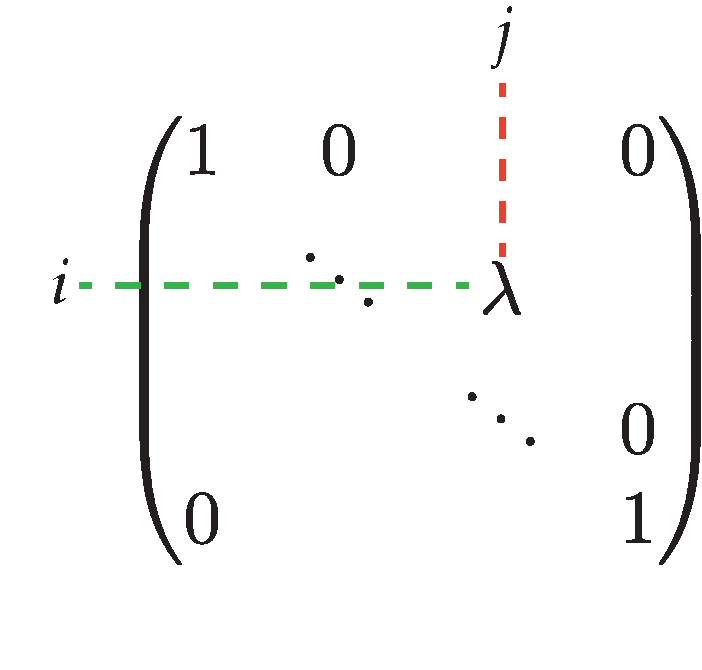
\includegraphics[scale=0.27]{Bilder/Matrix_Ei_j_lambda_2}}}
	\]
	\item Für $i \not= j$
	\[
		T(i,j) = \vcenter{\hbox{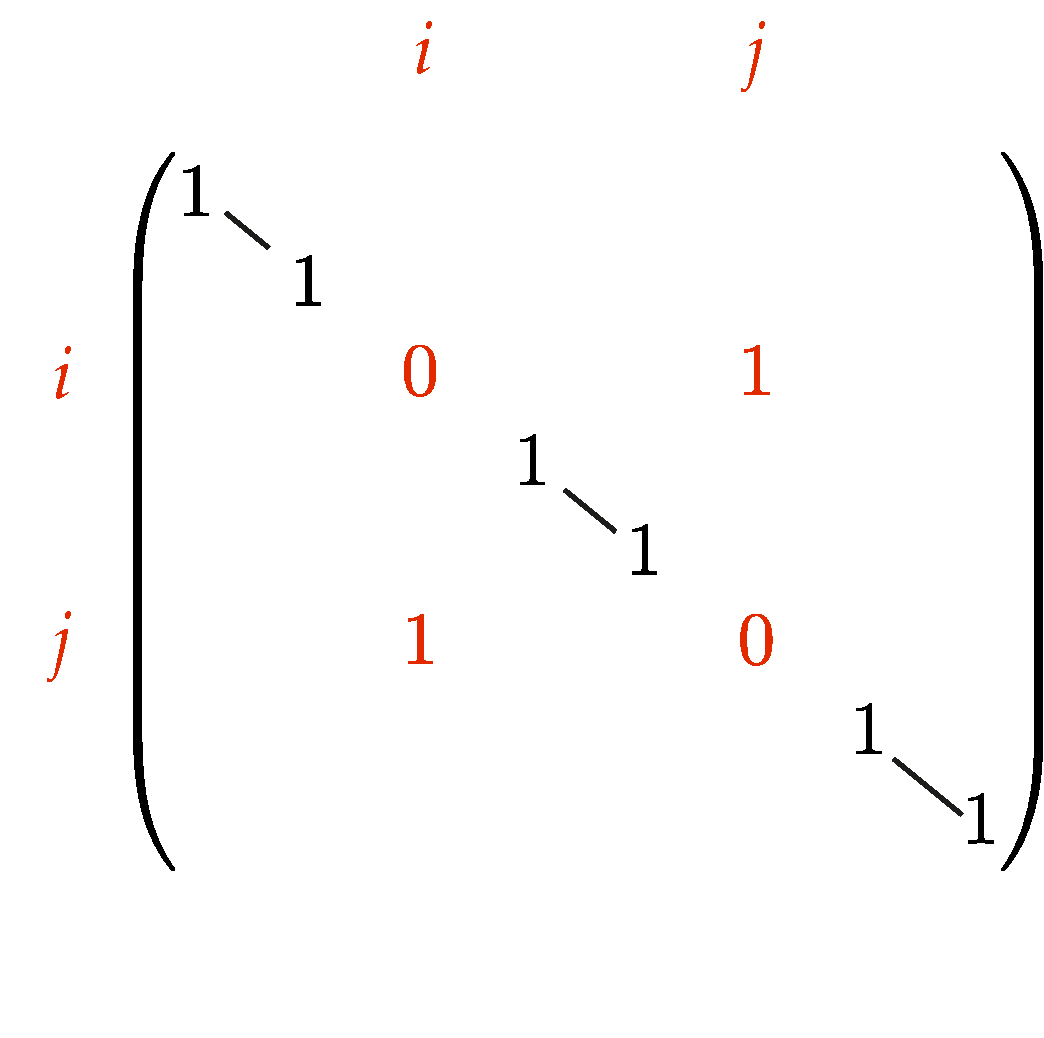
\includegraphics[scale=0.22]{Bilder/Matrix_T_i_j}}}
	\]
	\item Für $i \in \{ 1, \ldots , n \} , \lambda \not= 0  \in K$
	\[
		E(i, \lambda ) = \vcenter{\hbox{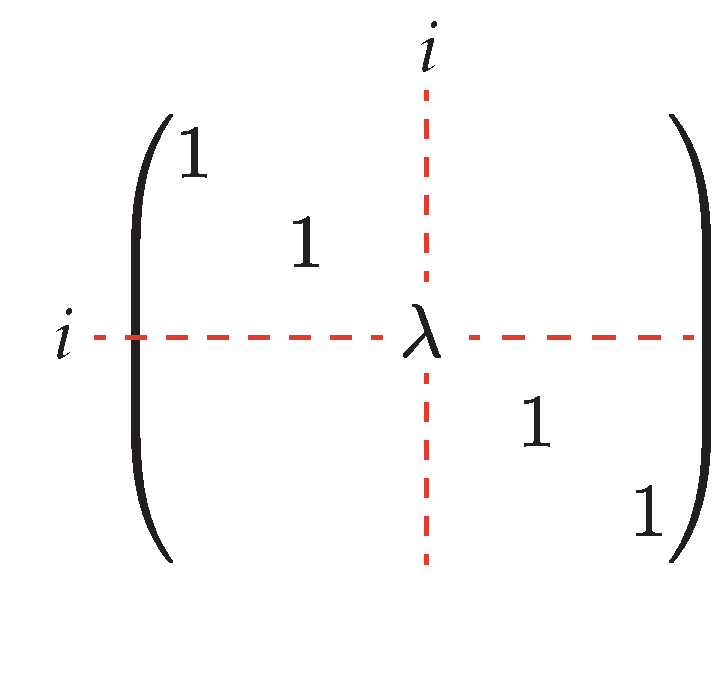
\includegraphics[scale=0.27]{Bilder/Matrix_E_i_lambda}}}
	\]
\end{enumerate}
% subsection defintion (end)

\subsection{Bemerkung} % (fold)
\label{sub:bemerkung}
\begin{enumerate}[a)]
	\item seien $z_1, \ldots , z_m$ die Zeilen der \(m \times n \)-Matrix  $A$. Also $A= \begin{pmatrix}
		z_1 \\ \cdot \\ z_n
	\end{pmatrix}$. Dann gelten
	\begin{enumerate}[I)]
		\item $E(i,j; \lambda )A = \begin{pmatrix}
			z_1 \\ \cdot \\ z_i + \lambda z_j \\ \cdot \\ z_j \\ \cdot \\ z_m
		\end{pmatrix}$
		\item  $T(i,j) \cdot A = \begin{pmatrix}
			z_1 \\ \cdot \\ z_j \\ \cdot \\ z_i \\ \cdot \\ z_m
		\end{pmatrix}$
		\item  $E(i, \lambda ) \cdot A = \begin{pmatrix}
			z_1, \\ \cdot \\ \lambda z_i \\ \cdot \\ z_m
		\end{pmatrix}$
	\end{enumerate}
	Die elementaren Umformungen von Gleichungssystemen entsprechen also der Linksmultiplikation mit Elementarmatrizen. Für Matrizen nennen wir diese
	(elementaren) \underline{\textbf{Zeilenumformungen}}
	\item Seien also $s_1, \ldots , s_n \in K^m$ die Spalten der \(m \times n \)-Matrix $A$. Also $A= (s_1, \ldots , s_n)$. Dann gelten
	\begin{enumerate}[I)]
		\item $A \cdot E(i,j; \lambda ) = (s_1, \ldots , s_j + \lambda s_i , \ldots , s_n)$
		\item $A \cdot T(i,j) = (s_1 \ldots  s_j  \ldots  s_i  \ldots  s_n)$
		\item $A \cdot E(i, \lambda ) = (s_1 \ldots  \lambda s_i \ldots s_n)$
	\end{enumerate}
	Diese Umformungen nennen wir  für Matrizen (elementare) \underline{\textbf{Spaltenumformungen}}.
\end{enumerate}
% subsection bemerkung (end)

\subsection{Bemerkung} % (fold)
\label{sub:bemerkung}
Die Elementarmatrizen sind invertierbar
\begin{align*}
	E(i,j; \lambda ) ^{-1} &= E (i,j; - \lambda ) \\
	T(i,j) ^{-1} &= T(i,j) \\
	E(i, \lambda ) ^{-1} &= E(i,\lambda ^{-1})
\end{align*}
% subsection bemerkung (end)

\subsection{Proposition} % (fold)
\label{sub:proposition}
Seien $A,B \in K^{m \times n}$ geht $B$ aus $A$ durch elementare Zeilen- und Spaltenumformungen hervor, so sind $A$ und $B$ äquivalent.
Insbesondere gilt
\[
	\text{Rang }A = \text{ Rang }B
\]
\underline{\textbf{Beweis:}} \\
Es git elementare Matrizen $E_1, \ldots , E_N$ $F_1, \ldots , F_M$ mit 
\[
	B= E_N \cdot \ldots \cdot E_2 \cdot E_1 \cdot A \cdot F_1 \cdot  F_2 \cdot \ldots \cdot F_M
\]
Also
\[
	S= (F_1 \cdot \ldots \cdot F_M) ^{-1} \in GL(n,K), T_i= E_N \cdot \ldots \cdot  E_1 \in GL(m.K)
\]
mit $B=T \cdot A \cdot S ^{-1}$ \hfill \( \square \)
% subsection proposition (end)

\subsection{Beispiel} % (fold)
\label{sub:beispiel}
Betrachte $A= \begin{pmatrix}
	1 & 2 & 3 \\
	2 & 3 & 4 \\
	3 & 4 & 5
\end{pmatrix}$ Durch elementare Umformungen erhalten wir:
\[
	\begin{pmatrix}
		1 & 2 & 3 \\
		2 & 3 & 4 \\
		3 & 4 & 5
	\end{pmatrix} \leadsto \begin{pmatrix}
		1 & 2 & 3 \\
		0 & -1 & -2 \\
		0 & -2 & -4
	\end{pmatrix} \leadsto \begin{pmatrix}
		1 & 2 & 3 \\
		0 & 1 & 2 \\
		0 & 2 & 4
	\end{pmatrix} \leadsto \begin{pmatrix}
		1 & 2 & 3 \\
		0 & 1 & 2 \\
		0 & 0 & 0 
	\end{pmatrix} \leadsto \begin{pmatrix}
		1 & 0 & 0 \\
		0 & 1 & 2 \\
		0 & 0 & 0
	\end{pmatrix} \leadsto \begin{pmatrix}
		1 & 0 & 0 \\
		0 & 1 & 0 \\
		0 & 0 & 0
	\end{pmatrix}
\]
Also $\text{Rang }A = \text{ Rang } \left( \begin{smallmatrix}
	1 & 0 & 0 \\
	0 & 1 & 0 \\
	0 & 0 & 0
\end{smallmatrix} \right) = 2$
% subsection beispiel (end)
% section matrizen (end)

\section{Die Spur} % (fold)
\label{sec:die_spur}

\subsection{Defintion} % (fold)
\label{sub:defintion}
Die \textbf{\underline{Spur}} einer quadratischen Matrix $A= (a_{ij}) \in K^{n \times n}$ ist 
\[
	\Sp (A) := \sum\limits_{i=1}^{n} a_{ii}
\]
Beispiel: $\Sp(I_r) = r$ , $\Sp \left( \begin{smallmatrix}
	1 & 2 & 3 \\
	2 & 3 & 4 \\
	3 & 4 & 5
\end{smallmatrix} \right) = 9$
% subsection defintion (end)

\subsection{Lemma} % (fold)
\label{sub:lemma}
\[
	\Sp (A B) = \Sp (B A)
\]
\underline{\textbf{Beweis:}} \\
Seien $A= (a_{ij}), B= (b_{ji}) \in K^{n \times n}$
\[
	\Sp (A B) = \sum\limits_{i=1}^{n} (i,i) \text{ Eintrag von } A \cdot B = \sum\limits_{i=1}^{n} \sum\limits_{j=1}^{n} a_{ij} b_{ji}
\]
\[
	= \sum\limits_{j=1}^{n} \sum\limits_{i=1}^{n} a_{ij} b_{ji} = \sum\limits_{j=1}^{n} \sum\limits_{i=1}^{n} b_{ji} a_{ij} = \sum\limits_{j=1}^{n} \sum\limits_{i=1}^{n} 
	(j,j)\text{-Eintrag von } B \cdot A = \Sp(B \cdot A)
\]
\hfill \( \square \)
% subsection lemma (end)

\subsection{Korollar} % (fold)
\label{sub:korollar}
Die Spuren ähnlicher Matrizen stimmen überein. 
\vspace{10pt} \\
\underline{\textbf{Beweis:}} \\
Sind $A,B \in K^{n \times n}$ ähnlich so gibt es $S \in Gl(n,K)$ mit 
\[
	S \cdot A \cdot S ^{-1} = B
\]
Damit folgt 
\[
	\Sp (B) = \Sp ( ( SA) S ^{-1}) \overset{9.2}{=} \Sp (S ^{-1} SA) = \Sp (A) 
\]
\hfill \( \square \)
% subsection korollar (end)

\subsection{Defintion} % (fold)
\label{sub:defintion}
Sei $f: V \to V$ ein Endomorphismus eines \(K\)-Vektorraumes endlicher Dimension. Die Spur von $f$ ist dann $\Sp (f) := \Sp ( m_B^B(f))$ für eine Basis $B$ von $V$
% subsection defintion (end)

\subsection{Bemerkung} % (fold)
\label{sub:bemerkung}
Die Spur von $f$ hängt nicht von der Wahl von $B$ ab: Ist $C$ eine zweite Basis von $V$ so sind $m_B^B(f)$ und $m_C^C (f)$ ähnlich und daher gilt
\[
	\Sp (m_B^B (f)) = \Sp (m_C^C(f)) 
\]
(siehe 9.3)
% subsection bemerkung (end)

\subsection{Bemerkung} % (fold)
\label{sub:bemerkung}
\[
	\Sp A = \Sp A^t 
\]
% subsection bemerkung (end)

\subsection{Satz} % (fold)
\label{sub:satz}
Sei $T : K^{n \times n} \to K $ eine linear Abbildung mit der Eigenschaft
\[
	T(A \cdot B) = T(B \cdot A) \quad \text{ für alle } A,B \in K^{n \times n}
\]
Dann ist $T$ ein skalares Vielfaches von $\Sp$ . Es gibt also $\lambda \in K$ mit 
\[
	T(A)= \lambda \Sp (A) \text{ für alle } A \in K^{n \times n}
\]
\underline{\textbf{Beweis:}} \\
Sei 
\[
	E_{ij} = \begin{pmatrix}
		 0 & \cdots & \cdots  & \cdots & 0  \\
		 \vdots & \ddots & & & \vdots \\
		  & & 1 & &   \\
		  \vdots &  &  &\ddots  &  \vdots \\
		 0 & \cdots & \cdots & \cdots & 0
	\end{pmatrix} \tag{an der stelle i,j 1}
\]
die Matrix, die an der Stelle $(i,j)$ eine 1 hat und sonst Nullen. Die $E_{ij}$ bilden eine Basis von $K^{n \times n}$.  Es gilt
\[
	E_{ij} E_{kl} = \begin{cases}
		E_{il}, &\text{ falls } j=k\\
		0 , &\text{ falls } j \not= k
	\end{cases}
\]
Für $i \not= l$ ist daher
\[
	E_{ij} E_{jl}- E_{jl} E_{ij} = E_{il}
\]
und folglich
\[
	T(E_{jl}) = T( E_{ij} E_{jl}- E_{jl} E_{ij} )
\]
\begin{align*}
	T(E_{jl}) &= T( E_{ij} E_{jl}- E_{jl} E_{ij} ) \\
	&= T(E_{ij} E_{jl})- T(E_{jl} E_{ij}) \\
	&= T(E_{ij} E_{jl}) - T( E_{ij} E_{jl}) = 0
\end{align*}
Wegen
\[
	E_{ij} E_{ji} - E_{ji} E_{ji} = E_{ii} E_{jj}
\]
gilt
\[
	T(E_{ii}) = T( E_{jj})
\]
Es folgt für $A= (a_{ij}) = \sum\limits_{i,j=1}^{n} a_{ij}E_{ij} $
\[
	T(A)= \sum\limits_{i,j=1}^{n} a_{ij} T(E_{ij}) = \sum\limits_{i=1}^{n} a_{ii}  T(E_{11})= T(E_{11}) \cdot  \Sp (A)
\]
Also
\[
	T= \lambda \Sp \text{ mit } \lambda = T(E_{11})
\]
\hfill \( \square \)
% subsection satz (end)

% section die_spur (end)

\section{Permutationen} % (fold)
\label{sec:permutatationen}

\subsection{Definition} % (fold)
\label{sub:definition}
Sei $n \in \mathds{N} $ $S_n= \{ \sigma : \{ 1, \ldots , n\} \to \{ 1, \ldots , n\} \mid \sigma \text{ ist bijektiv}\}$ heißt die 
\underline{\textbf{symmetrische Gruppe}} zum Index $n$. Elemente von $S_n$ heißen \underline{\textbf{Permutationen}}.
% subsection definition (end)

\subsection{Notation} % (fold)
\label{sub:notation}
Oft schreibt man
\[
	\sigma = \begin{pmatrix}
		1 & 2 & \cdots & n \\
		\sigma(1) & \sigma(2) & \cdots & \sigma(n)
	\end{pmatrix}
\]
% subsection notation (end)

\subsection{Beispiel} % (fold)
\label{sub:beispiel}
\[
	\begin{pmatrix}
		1 & 2 & 3 \\
		2 & 3 & 1
	\end{pmatrix} \in S_3
	\quad \begin{pmatrix}
		1 & 2 & 3 & 4 \\
		2 & 1 & 4 & 3
	\end{pmatrix} \in S_4
	\quad \begin{pmatrix}
		1 & 2 & 3 & 4 \\
		4 & 2 & 3 & 2
	\end{pmatrix} \not\in S_4
\]
% subsection beispiel (end)
\subsection{Notation} % (fold)
\label{sub:notation}
Seien $i,j \in \{ 1, \ldots , n\}$ mit $i \not= j$. Dann schreibt man $(i,j)$ für Permutationen $\sigma \in S_n$ mit 
\[
	\sigma (k) = \begin{cases}
		i, &\text{ falls } k=j\\
		j , &\text{ falls } k=i \\
		k , &\text{ sonst}
	\end{cases}
\]
Permutationen dieser Form heißen \underline{\textbf{Transpositionen}}
% subsection notation (end)

\subsection{Bemerkung} % (fold)
\label{sub:bemerkung}
\begin{enumerate}[(i)]
	\item $S_1$ ist die neutrale Gruppe
	\item $S_2$ besteht genau aus zwei Elementen: Der Identität und der Transposition $(1,2)$
	\item $S_3$ ist nicht abelsch. 
	\[
		(1,2)(2,3)= \begin{pmatrix}
				1 & 2 & 3 \\
				2 & 3 & 1
			\end{pmatrix} 
		\qquad (2,3)(1,2)= \begin{pmatrix}
			1 & 2 & 3 \\
			3 & 1 & 2
		\end{pmatrix}
	\]
	
\end{enumerate}
Genauso ist $S_n$ für $n \ge 3$ nicht abelsch
% subsection bemerkung (end)

\subsection{Defintion} % (fold)
\label{sub:defintion}
Sei $\sigma \in S_n$. Sei $k$ die Anzahl der zwei-elementiger Teilmengen $\{ i,j\} \subseteq \{ 1, \ldots , n \}$ mit $i <j$ und $\sigma(i)> \sigma(j)$.
Dann heißt 
\[
	\text{sgn}(\sigma) := (-1)^k
\]
Das \underline{\textbf{Signum}} von $\sigma$
% subsection defintion (end)

\subsection{Beispiel} % (fold)
\label{sub:beispiel}
Ist $\sigma$ eine Transposition, so ist
\[
	\text{sgn}(\sigma) = -1
\]
% subsection beispiel (end)

\subsection{Bemerkung} % (fold)
\label{sub:bemerkung}
\begin{enumerate}[(i)]
	\item 
	\[
		\text{sgn}(\sigma)= \prod\limits_{1 \le i < j \le n} \frac{\sigma(j)- \sigma(i)}{j-i} \tag{$= 1 \vee -1$}
	\]
	\item Sei $P$ die Menge aller Paare $(i,j)$ mit $i,j \in \{ 1, \ldots , n\} , i \not= j$. \\
	Ein \underline{\textbf{Halbsystem}} ist eine Teilmenge von $P$, die von den Paaren $(i,j)$ und $ (j,i)$ jeweils genau eins enthält. Dann gilt für jedes
	Halbsystem
	\[
		\text{sgn}(\sigma)= \prod\limits_{(i,j) \in H} \frac{\sigma(j)- \sigma(i)}{j-i} 
	\]
	\item Ist $H$ ein Halbsystem und $\tau \in S_n$ so ist auch $\tau H := \Big\{ \big( \tau(i), \tau(j) \big) \mid (i,j) \in H \Big\}$ ein Halbsystem und es gilt
	\[
		\sgn(\sigma) = \prod\limits_{(i,j) \in \tau H} \frac{\sigma(j)- \sigma(i)}{j-i} = \prod\limits_{(i,j) \in H} 
		\frac{\sigma(\tau(j))- \sigma(\tau(i))}{\tau(j)-\tau(i)}  
	\]
\end{enumerate}
% subsection bemerkung (end)

\subsection{Lemma} % (fold)
\label{sub:lemma}
\[
	\sgn : S_n \to \{ \pm 1\}
\]
ist ein Gruppenhomomorphismus, das heißt $\sigma, \tau  \in S_n$ ist 
\[
	\sgn(\sigma \tau)= \sgn(\sigma) \cdot \sgn(\tau)
\]
\underline{\textbf{Beweis:}} \\
\begin{align*}
\sgn(\sigma \tau) &= \prod\limits_{(i,j)\in H} \frac{\sigma(\tau(j)) - \sigma( \tau (i))}{j-i} \\
 &= \prod\limits_{(i,j) \in H} \frac{\sigma(\tau(j)) - \sigma( \tau (i))}{\tau(j)- \tau(i)} \cdot \frac{\tau (j) - \tau(i)}{j-i}  \tag{erweitern}\\
&= \prod\limits_{(i,j)\in H} \frac{\sigma(\tau(j))- \sigma(\tau(i))}{\tau(j)- \tau(i)} \cdot \prod\limits_{(i,j) \in H} 
\frac{\tau(j)- \tau(i)}{j-i} \\ &= \sgn(\sigma)\cdot \sgn(\tau)  
\end{align*}
\hfill \( \square \)
% subsection lemma (end)

\subsection{Definition} % (fold)
\label{sub:definition}
\[
	A_n := \Big\{ \sigma \in S_n \mid \sgn(\sigma)=1 \Big\} = \text{Kern}(\sgn)
\]
heißt die \underline{\textbf{alternierende Gruppe}} vom Index $n$.
% subsection definition (end)

\subsection{Satz} % (fold)
\label{sub:satz}
\[
	| S_n | = n! 
\]
% subsection satz (end)

\subsection{Bezeichnung} % (fold)
\label{sub:bezeichnung}
Sei $H$ eine Untergruppe von $G$. Dann heißt $[G : H]= \left| \nicefrac{G}{H} \right| \in \mathds{N} \cup \{ \infty\}$ der \underline{\textbf{Index}} von $H$ in $G$.
% subsection bezeichnung (end)

\subsection{Satz von Lagrange} % (fold)
\label{sub:satz_von_lagrange}
Sei $H$ eine Untergruppe der endlichen Gruppe $G$ Dann gilt:
\[
	| G| = [G : H] \cdot  |H|
\]
\underline{\textbf{Beweis:}} \\
$G$ ist die disjunkte Vereinigung der Linksnebenklassen $gH$. Für jede Linksnebenklasse ist $h \mapsto gh$ eine bijektive Abbildung $H \to gH$
Insbesondere $| H| = |gH|$. \\
Es folgt
\[
	 |G| = \left|  \bigcup\limits_{gH \in \nicefrac{G}{H}}^{.} gH \right| = \sum\limits_{gH \in \nicefrac{G}{H}} |gH| = 
	 \sum\limits_{gH \in \nicefrac{G}{H}} |H| = | \nicefrac{G}{H}| \cdot |H|= [G : H] \cdot |H|
\]
\vspace{\baselineskip} \\
\underline{\textbf{Beweis von 10.11:}} \\
Durch Induktion nach $n$: \\
\textbf{I.A.:} Für $n=1$ ist $|S_1| = 1 = 1!$ \\
\textbf{I.S.:} $(n-1) \mapsto n$ Die Untergruppe $H= \{ \sigma \in S_n \mid \sigma(n)=n \}$ ist isomorph zu $S_{n-1}$
\vspace{10pt} \\
Nach Induktionsannahme gilt:
\[
	|H|= |S_{n-1}| = (n-1)!
\]
Für $\sigma, \tau  \in S_n$ gilt $\sigma H = \tau H$ genau dann wenn $\tau ^{-1} \sigma \in H$. Es gilt
\[
	\tau ^{-1} \sigma \in H \quad \Leftrightarrow \quad \tau ^{-1} \sigma(n)= n \quad \Leftrightarrow \quad \sigma(n)= \tau(n)
\]
Es folgt $[S_n : H] = n$
\[
	\overset{\text{Lagrange}}{\Rightarrow } |S_n| = [S_n : H] \cdot  |H| = n \cdot (n-1)!= n!
\]
\hfill \( \square \)
\vspace{\baselineskip} \\
{ \large \textbf{\underline{Satz}} }
\vspace{10pt} \\
Jede Permutation $\sigma \in S_n$ lässt sich als Produkt von Transpositionen schreiben.
\vspace{10pt} \\
\underline{\textbf{Beweis:}} durch Induktion nach $n$
\vspace{10pt} \\
I.A.: $n=1 , S_1= \{ \id \}$ $\id$ ist das leere Produkt von Transpositionen. 
\vspace{10pt} \\
I.S.: $(n-1) \mapsto n$. Sei $H= \{ \sigma \in S_n \mid \sigma(n)=n \} \cong S_{n-1}$. Per Induktionsannahme ist jedes Element von $H$ ein Produkt von Transpositionen. \\
Sei $\sigma \in S_n$. Ist $\sigma \in H$ so sind wir fertig. \\
Ist $\sigma \not\in H$ so $\sigma(n) \not= n$. Sei $\tau = (n \sigma(n)) \in S_n$ Dann gilt $\tau \circ \sigma \in H$. Also gibt es Transpositionen 
$\tau_1 , \ldots , \tau_l$ mit 
\[
	\tau \cdot  \sigma = \tau_1 \cdot \ldots \cdot \tau_n
\]
Dann ist auch $\sigma = \tau ^{-1} \tau_1 \ldots  \tau_n = \tau \tau_1 \cdots \tau_n$ ein Produkt von Transpositionen. \hfill \( \square \)
% subsection satz_von_lagrange (end)

\subsection{Korollar} % (fold)
\label{sub:korollar}
Für $\sigma\in S_n$ gilt $\sgn(\sigma)=1$ genau dann, wenn $\sigma$ ein Produkt einer gerade Zahl von Transpositionen ist und $\sgn(\sigma)= -1$ genau dann,
wenn $\sigma$ ein Produkt einer ungeraden Zahl von Transpositionen ist.
% subsection korollar (end)
% section permutatationen (end)

\section{Determinanten} % (fold)
\label{sec:determinanten}

\subsection{Definition} % (fold)
\label{sub:definition}
Sei $V$ ein Vektorraum. Eine Abbildung $D: V^n \to K$ heißt \underline{\textbf{$n$-linear}} oder eine \underline{\textbf{$n$-Linearform}}, wenn sie in jeder
Variable linear ist, wenn also immer gilt:
\[
	D(v_1, \ldots , v_i + v'_i , \ldots , v_n) = D(v_1, \ldots , v_i , \ldots , v_n) + D(v_1, \ldots , v'_i , \ldots , v_n)
\]
\[
	D(v_1, \ldots , \lambda v_i , \ldots v_n) = \lambda D(v_1, \ldots , v_i , \ldots , v_n)
\]
Eine $n$-Linearform heißt \underline{\textbf{alternierend}}, wenn aus $v_i = v_j$ mit $i \not= j$ immer 
\[
	D(v_1, \ldots , v_i , \ldots , v_j , \ldots , v_n)=0.
\]
folgt. \\
Sei $\text{Alt}^n (V)$ die Menge der alternierenden $n$-Linearformen auf $V$. $\alt^n (V)$ wird durch Addition und skalare Multiplikation der Funktionswerte zu einem
Vektorraum.
\[
	(D+D') (v_1, \ldots , v_n) = D(v_1, \ldots , v_n) + D'(v_1, \ldots , v_n)
\]
\[
	(\lambda D) (v_1, \ldots , v_n) = \lambda D(v_1, \ldots , v_n)
\]

% subsection definition (end)

\subsection{Propositon} % (fold)
\label{sub:propositon}
Sei $D \in \alt^n(V)$
\begin{enumerate}[(i)]
	\item Ist $i \not= j$, $\lambda  \in K$ so gilt 
	\[
		D(v_1, \ldots , v_i, \ldots , v_j , \ldots , v_n) = D(v_1, \ldots , v_i + \lambda v_j, \ldots , v_j , \ldots  , v_n)
	\]
	\item Ist $i\not= j$ so gilt
	\[
		D(v_1, \ldots , v_i , \ldots , v_j , \ldots , v_n)= - D(v_1, \ldots , v_j , \ldots , v_i , \ldots , v_n)
	\]
	\item Ist $v_1, \ldots , v_n$ linear abhängig, so gilt
	\[
		D(v_1, \ldots , v_n) = 0
	\]
\end{enumerate}
\underline{\textbf{Beweis:}} \\
Um die Notation zu vereinfachen, nehmen wir für (i) und (ii) an. $n=2$, $i=1$, $j=2$
\begin{enumerate}[(i)]
	\item $D(v_1 + \lambda v_2 , v_2) = D(v_1 , v_2)+ D(\lambda v_2 , v_2) = D(v_1, v_2)+ \lambda \underbrace{D(v_2 , v_2)}_{=0} = D(v_1 , v_2)$
	\item $0= D(v_1 + v_2, v_1 + v_2)= D(v_1, v_1 + v_2)+ D(v_2, v_1 + v_2) = \underbrace{D(v_1, v_1)}_{=0}+ D(v_1, v_2)+ D(v_2, v_1)+ \underbrace{D(v_2, v_2)}_{=0}$ \\
	Also $0= D(v_1, v_2)+ D(v_2, v_1)$ \\
	Also $D(v_1, v_2)= - D(v_2, v_1)$
	\item Ist $v_i = \sum\limits_{i \not= j} \lambda_j v_j 	 $ so folgt
	\[
		D(v_1, \ldots , v_i, \ldots , v_n) = D(v_1, \ldots , \sum\limits_{i \not= j} \lambda_j v_j , \ldots , v_n ) = \sum\limits_{i \not= j}\lambda_j 
		\overbrace{D(v_1, \ldots , v_j , \ldots , v_n)}^{=0} = 0
	\]
\end{enumerate}
\hfill \( \square \)
% subsection propositon (end)

\subsection{Beispiel} % (fold)
\label{sub:beispiel}
$V=K^m$
\begin{enumerate}[(i)]
	\item $D : (K^m)^n \to K$ mit 
	\[
		D \left(\begin{pmatrix}
			a_{11} \\ \vdots \\ a_{m1}
		\end{pmatrix} , \ldots , \begin{pmatrix}
			a_{1n} \\ \vdots \\ a_{mn}
		\end{pmatrix} \right) = a_{i1} \cdot a_{i2} \cdot \ldots \cdot a_{in}
	\]
	ist für $i \in \{ 1, \ldots , m\}$ eine $n$-Linearform
	\item Sei $f : \{1, \ldots , n \} \to \{ 1, \ldots , n \}$ eine Abbildung. Sei $\sigma \in S_n$. Dann ist 
	\[
		D : (K^n)^n \to K \enspace \text{ mit } \enspace D \left( \begin{pmatrix}
			a_{11} \\ \vdots \\ a_{n1}
		\end{pmatrix}, \ldots , \begin{pmatrix}
			a_{1n} \\ \vdots \\ a_{nn}
		\end{pmatrix} \right) = a_{1 \sigma(1)} \cdot a_{2 \sigma(2)} \cdot \ldots \cdot a_{n \sigma(n)}
	\]
	eine $n$-Linearform
	\item \[
		D : (K^n)^n \to K \text{ mit } D= \sum\limits_{\sigma \in S_n } \sgn(\sigma) D_{\sigma}
	\]
	ist eine alternierende $n$-Linearform. Seien $r,s \in \{ 1, \ldots ,n \}$ , $ r \not= s$ mit $\begin{pmatrix}
		a_{1r} \\ \vdots \\ a_{nr}
	\end{pmatrix} = \begin{pmatrix}
		a_{1s} \\ \vdots \\ a_{ns}
	\end{pmatrix}$.
	\vspace{10pt} \\
	Sei $ \tau = (r,s) \in S_n$. Dann gilt
	\[
		D_\sigma \left( \begin{pmatrix}
			a_{11} \\ \vdots \\ a_{n1}
		\end{pmatrix} , \ldots , \begin{pmatrix}
			a_{1n} \\ \vdots \\ a_{nn}
		\end{pmatrix} \right) = 
		D_{\tau \circ \sigma} \left( \begin{pmatrix}
			a_{11} \\ \vdots \\ a_{n1}
		\end{pmatrix} , \ldots , \begin{pmatrix}
			a_{1n} \\ \vdots \\ a_{nn}
		\end{pmatrix} \right)
	\]
	Da $S_n$ die disjunkte Vereininung von $A_n$ mit $\tau A_n$ ist, folgt und $\sgn(\sigma)= - \sgn(\tau \sigma)$
	\begin{align*}
		& D \left( \begin{pmatrix}
			a_{11} \\ \vdots \\ a_{n1}
		\end{pmatrix} , \ldots , \begin{pmatrix}
			a_{1n} \\ \vdots \\ a_{nn}
		\end{pmatrix} \right) \\
		= & \sum\limits_{\sigma \in A_n} D_\sigma \left( \begin{pmatrix}
			a_{11} \\ \vdots \\ a_{n1}
		\end{pmatrix} , \ldots , \begin{pmatrix}
			a_{1n} \\ \vdots \\ a_{nn}
		\end{pmatrix} \right) - \sum\limits_{\sigma \in A_n} D_{\tau \circ \sigma} \left( \begin{pmatrix}
			a_{11} \\ \vdots \\ a_{n1}
		\end{pmatrix} , \ldots , \begin{pmatrix}
			a_{1n} \\ \vdots \\ a_{nn}
		\end{pmatrix} \right) \\
		= & \sum\limits_{\sigma \in A_n} ( D_\sigma - D_{\tau \circ \sigma}) \left( \begin{pmatrix}
			a_{11} \\ \vdots \\ a_{n1}
		\end{pmatrix} , \ldots , \begin{pmatrix}
			a_{1n} \\ \vdots \\ a_{nn}
		\end{pmatrix} \right) = 0
	\end{align*}
	\[
		D \left( \begin{pmatrix}
			a_{11} \\ \vdots \\ a_{n1}
		\end{pmatrix} , \ldots , \begin{pmatrix}
			a_{1n} \\ \vdots \\ a_{nn}
		\end{pmatrix} \right) := \sum\limits_{\sigma \in S_n} \sgn(\sigma) a_{1 \sigma(1)} \cdot \ldots \cdot a_{n \sigma(n)}
	\]
	Für die Standardbasis $e_1, \ldots , e_n$ von $K^n$ gilt 
	\[
		D ( e_1, \ldots , e_n) = \sum\limits_{\sigma \in S_n} \sgn(\sigma) {\delta_{1 \sigma(i)} \cdot \ldots \cdot \delta_{n \sigma(n)}}_{= 1 \text{ für } \sigma = \id}
		 = 1
	\]
	wobei $\delta_{1 \sigma(1)}, \ldots , \delta_{n \sigma(n)} = \begin{cases}
		1, &\text{ falls } \sigma = \id \\
		0, &\text{ sonst}
	\end{cases}$ \\
	mit
	\[
		\delta_{ij} = \begin{cases}
			1, &\text{ falls } i=j\\
			0 , &\text{ falls } i \not= j
			
		\end{cases} \qquad e_i = \begin{pmatrix}
			\delta_{i1} \\ \vdots \\ \delta_{in}
		\end{pmatrix}
	\]
	
	hier fehlt noch was…
\end{enumerate}
% subsection beispiel (end)

\subsection{Bemerkung} % (fold)
\label{sub:bemerkung}
Ist $\dim V < n $ so ist $\alt^n (V) = 0$ wegen 11.2 (iii)
% subsection bemerkung (end)

\subsection{Satz} % (fold)
\label{sub:satz}
Ist $\dim V = n$ so ist $ \dim \alt^n(V) = 1$
\vspace{\baselineskip} \\
\underline{\textbf{Beweis:}} \\
Sei $D \in \alt^n (V)$. Sei $b_1, \ldots , b_n$ eine Basis von $V$. Dann schreiben wir
\[
	v_i = \sum\limits_{j=1}^{n} \lambda _{ij} b_j \quad \text{ mit } \lambda_{ij} \in K
\]
Es folgt
\begin{align*}
	D(v_1, \ldots , v_n) &= D \left( \sum\limits_{j=1}^{n}  \lambda_{1j} b_j , \ldots , \sum\limits_{j=1}^{n} \lambda_{nj} b_j  \right) \\
	&= \sum\limits_{j_1, \ldots , j_n \in \{ 1, \ldots , n \} } \lambda_{1 j_1} \cdot  \lambda_{2 j_2} \cdot  \ldots \cdot  \lambda_{n j_n}
	D(b_{j_1} , \ldots , b_{j_n})
\end{align*}
Ist $j_i = j_k$ für $i \not= k$ so ist $D(b_{j_1} , \ldots , b_{j_n})= 0$. Daher ist $\begin{pmatrix}
	1 & 2 & \ldots & n \\
	j_1 & j_2 & \ldots & j_n
\end{pmatrix}$ eine Permutation wenn $D(b_{j_1} , \ldots , b_{j_n}) \not= 0$ ist. Wir erhalten
\begin{align*}
	D(v_1, \ldots , v_n) &= \sum\limits_{\sigma \in S_n} \lambda_{1 \sigma(1)} \cdot  \ldots \cdot \lambda_{n \sigma(n)} \cdot D( b_{\sigma(1)} , \ldots , b_{\sigma(n)})\\
	&= \sum\limits_{\sigma \in S_n} \lambda_{1 \sigma(1)} \cdot \ldots \cdot \lambda_{n \sigma(n)} \cdot \sgn(\sigma) \cdot D(b_1, \ldots, b_n)
\end{align*}
Daher ist $D$ durch seinen Wert auf $(b_1, \ldots , b_n)$ eindeutig festgelegt und es folgt
\[
	\dim ( \alt^n(V)) \le 1
\]
etwas formaler: Betrachte $\varphi : \alt^n(V) \to K$ mit $\varphi(D) := D(b_1, \ldots , b_n)$. Dies ist eine lineare Abbildung und die obige Überlegung zeigt,
dass $\varphi$ injektiv ist. Also $\dim \alt^n(V) \le 1$
\vspace{10pt} \\
Es bleibt zu zeigen $\alt^n(V) \not= \{ 0\}$. Für $V=K^n$ haben wir schon $D \not= 0$ in 11.3 (iii) konstruiert. Ist nun
\[
	\kappa : V \to K^n
\]
ein Isomorphismus, so wird durch $\tilde D(v_1, \ldots , v_n) := D(\kappa(v_1), \ldots , \kappa(v_n))$ ein nicht-triviales Element in $\alt^n(V)$ definiert. 
\hfill \( \square \)
% subsection satz (end)

\subsection{Satz} % (fold)
\label{sub:satz}
Sei $f: V \to V$ $K$-linear, wobei $\dim_K V = n$. Dann gibt es ein eindeutiges $\lambda \in K$, so dass
\[
	D \big(f(v_1). \ldots , f(v_n)\big) = \lambda \cdot D(v_1, \ldots , v_n)
\]
für alle $v_1, \ldots , v_n \in V$ , $D \in \alt^n(V)$ 
\vspace{\baselineskip} \\
\underline{\textbf{Beweis:}} \\
Wir schreiben $f^*D$ für die alternierende $n$-Form $(v_1, \ldots , v_n) \mapsto D \big(f(v_1). \ldots , f(v_n)\big)$.
\vspace{10pt} \\
Wähle $D \not= 0$ in $\alt^n(V)$. Da $\dim \alt^n(V)=1$ ist $D$ schon eine Basis von $\alt^n(V)$. Daher gibt es ein eindeutiges $\lambda \in K$ mit 
\[
	f^* D = \lambda D
\]
Sei nun $D' \in \alt^n(V)$ beliebig. Da $D$ Basis von $\alt^n(V)$, gibt es $\mu \in K$ mit $D'= \mu D$. Es folgt
\begin{align*}
	D' \big( f(v_1), \ldots , f(v_n)\big) &= \mu D \big(f(v_1). \ldots , f(v_n)\big)  \\
	&= \mu (f^* D (v_1, \ldots , v_n)) \\
	&= \mu \cdot \lambda \cdot D (v_1, \ldots , v_n) \\
	&= \lambda \mu D (v_1, \ldots , v_n) = \lambda D' (v_1, \ldots , v_n)
\end{align*}
\hfill \( \square \)
% subsection satz (end)

\subsection{Definition} % (fold)
\label{sub:definition}
$\lambda $ aus 11.6 heißt die \underline{\textbf{Determinante}} von $f$, geschrieben 
\[
	\det (f)
\]
\underline{Beispiel:} \\
\[
	\det (\id_V) = 1 \qquad \det (0)= 0
\]
% subsection definition (end)

\subsection{Satz} % (fold)
\label{sub:satz}
Sei $\dim V = n$. Dann gilt für $f,g  \in \text{ End}_K (V)$
\[
	  \det (f \circ g) = \det (f) \cdot \det (g)
\]
\underline{\textbf{Beweis:}} \\
Für $D \in \alt^n(V)$ , $v_1, \ldots , v_n \in V$ gilt
\begin{align*}
	D \big(f \circ g (v_1), \ldots , f \circ g (v_n) \big) &= D \big(f ( g (v_1)), \ldots , f ( g (v_n)) \big) \\
	&= \det (f) \cdot D \big( g(v_1), \ldots , g(v_n) \big) \\
	&= \det(f) \cdot \det (g) \cdot D(v_1, \ldots , v_n)
\end{align*}
Also 
\[
	\det (f \circ g) = \det (f) \cdot \det (g)
\]
% subsection satz (end)

\subsection{Korollar} % (fold)
\label{sub:korollar}
Sei $\dim V = n$. Für $f \in \text{ End}_K (V)$ sind äquivalent
\begin{enumerate}[(i)]
	\item $\det (f) \not= 0$
	\item $f$ ist invertierbar
\end{enumerate}
In diesem Fall gilt $\det (f ^{-1}) = \det (f) ^{-1}$
\vspace{\baselineskip} \\
\underline{\textbf{Beweis:}} \\
\underline{"' ii) $\Rightarrow $ i)"' }
\vspace{10pt} \\
\[
	1 = \det (\id_V) = \det ( f \circ f ^{-1}) = \det (f) \cdot \det (f ^{-1})
\]
Es folgt $\det (f ^{-1}) \not= 0$ , genauer gilt 
\[
	\det (f ^{-1}) = \det (f) ^{-1}
\]
\underline{"' $\neg$ ii) $\Rightarrow $ $\neg$ i)"' } \\
Sei $f$ nicht invertierbar. Dann ist 
\[
	\dim \text{ Bild }f < n
\]
Insbesondere ist für $v_1, \ldots , v_n \in V$ $f(v_1), \ldots , f(v_n)$ linear abhängig. Dann gilt für $D \in \alt^n(V)$
\[
	D(f(v_1), \ldots , f(v_n)) = 0
\]
Das heißt $\det (f) = 0$
% subsection korollar (end)

\subsection{Definition} % (fold)
\label{sub:definition}
Sei $A \in K^{n \times n}$. Die Determinante von $A$ ist die Determinante der zugehörigen Abbildung $f_A : K^n \to K^n$ , $v \mapsto A \cdot v$
\[
	\det (A) := \det (f_A)
\]
% subsection definition (end)

\subsection{Proposition} % (fold)
\label{sub:proposition}
Seien $A,B \in K^{n \times n}$
\begin{enumerate}[(i)]
	\item $\det (AB)= \det (A) \cdot \det(B)$
	\item $A$ ist genau dann invertierbar, wenn $\det A \not= 0$ \\
	In diesem Fall ist
	\[
		\det (A ^{-1}) = ( \det A) ^{-1}
	\]
	\item Sind $A$ und $B$ ähnlich, so ist $\det A = \det B$
\end{enumerate}
\underline{\textbf{Beweis:}} \\
\begin{enumerate}[(i)]
	\item folgt aus 11.8, da $f_{A \cdot B} = f_A \circ f_B$
	\item folgt aus 11.9, da $(f_A) ^{-1} = f_{A ^{-1}}$
	\item folgt aus (i) und (ii): \quad $A$ und $B$ ähnlich $\Rightarrow \exists S \in Gl(n,K)$ mit
	\[
		A = S B S ^{-1}
	\] 
	Also
	\[
		\det A = \det ( SBS ^{-1}) = \det S \cdot \det B \cdot \underbrace{\det (S ^{-1})}_{= (\det S) ^{-1}} = \det B
	\]
\end{enumerate}

% subsection proposition (end)

\subsection{Proposition} % (fold)
\label{sub:proposition}
Sei $D \in \alt^n(K^n)$ wie in 11.3 (iii). Seien $s_1, \ldots , s_n \in K^n$ die Spalten von $A \in K^{n \times n}$. Also $	A= (s_1, \ldots , s_n)$.
Dann gilt 
\[
	\det (A) = D( s_1, \ldots , s_n)
\]
\underline{\textbf{Beweis:}} \\
Sei $e_1. \ldots , e_n$ die Standardbasis von $K^n$. Da $D(e_1, \ldots , e_n) = 1$ (siehe 11.3 (iii)) folgt 
\[
	\det A = \det A D(e_1, \ldots , e_n) = D(Ae_1 , \ldots , Ae_n) = D(s_1, \ldots , s_n)
\]
\hfill \( \square \)
% subsection proposition (end)

\subsection{Proposition} % (fold)
\label{sub:proposition}
$\det : K^{n \times n} \to K$ ist die eindeutige Abbdildung die eine alternierende $n$-Form in den Spalten ist und $\det (I_n)=1$ erfüllt.
\vspace{\baselineskip} \\
\underline{\textbf{Beweis:}} \\
Wegen 11.12 ist $\det : K^{n \times n} \to K$ eine alternierende $n$-Form in den Spalten und erfüllt $\det (I_n)=1$. Der Vektorraum $\alt^n(V)$ ist 1-dimensional.
Da außerdem $\det (I_n)=1$, legt dies die Determinante $\det$ eindeutig fest. \hfill \( \square \)
% subsection proposition (end)

\subsection{Bezeichnung} % (fold)
\label{sub:bezeichnung}
Für $A \in K^{n \times n}$ bezeichne $A_{ik}$ die aus $A$ durch Streichen der $i$-ten Zeile und $k$-ten Spalte entstehende $(n-1) \times (n-1)$-Matrix
\[
	\text{ Zeichnung eventuell}
\]
% subsection bezeichnung (end)

\subsection{Entwicklung nach der $k$-ten Zeile} % (fold)
\label{sub:entwicklung_nach_der_k_tem_spalte}
Für $A= (a_{ij}) \in K^{n \times n}$ , $k \in \{ 1, \ldots , n \}$ gilt
\[
	\star \qquad \det A = \sum\limits_{j=1}^{n} (-1)^{j+k} a_{kj} \det A_{kj}
\]
\underline{\textbf{Beweis:}} \\
Definiere $D : K^{n \times n} \to K$ durch die rechte Seite von $(\star)$. Wegen 11.13 genügt es zu zeigen, dass 
\begin{enumerate}[a)]
	\item $\det(I_n) = 1$
	\item $D$ ist $n$-linear
	\item $D$ ist alternierend
\end{enumerate}
\underline{zu a)} \\
Sei $I_n = (\delta_{ij})$. Dann 
\[
		D(I_n)= \sum\limits_{j=1}^{n}(-1)^{j+k} \delta_{jk} \det ( (I_n)_{kj}) = (-1)^{2k} \det (I_{n-1}) = 1
\]
\underline{zu b)} \\
$D$ ist linear da $A \mapsto a_{jk} \cdot \det (A_{jk})$ $n$-linear ist.
\vspace{10pt} \\
\underline{zu c)} \\
Sei $A=(s_1, \ldots , s_n)$ mit $s_r= s_t$ für $r <t$. Für $j \not\in \{ r,t \}$ ist $\det (A_{kj})=0$ da $A_{kj}$ zwei gleiche Spalten hat. Also
\begin{align*}
		D(A) &= (-1)^{r+k} a_{kr} \det (A_{kr}) + (-1)^{t+k} a_{kt} \det (A_{kt})  \\
		& \underset{a_{kr}=a_{kt}}{=} (-1)^k a_{kr} \Big( (-1)^r \det A_{kr} + (-1)^t \det A_{kt} \Big) 
\end{align*}
Ist $t= r+1$, so ist $A_{kr}= A_{kt}$. Andernfalls entsteht $A_{kt}$ durch $t-r-1$ Spaltenvertauschungen aus $A_{kr}$ und es folgt
\[
	\det (A_{kt})= (-1)^{t-r-1} \det (A_{kr})
\]
Damit erhalten wir 
\[
	D(A)= (-1)^k a_{kr} \det (A_{kr}) \Big( (-1)^r + (-1)^t \cdot (-1)^{t-r-1} \Big) = 0
\]
\hfill \( \square \)
% subsection entwicklung_nach_der_k_tem_spalte (end)

\subsection{Beispiel} % (fold)
\label{sub:beispiel}
\begin{enumerate}[(i)]
	\item $n=1$ , $\det(a)=a$
	\item $n=2$ , $\det( \begin{smallmatrix}
		a & b \\
		c & d
	\end{smallmatrix}) = a \det (d) - b \det (c) = ad -bc$
	\item $n=3$
	\begin{align*}
		\det \begin{pmatrix}
			1 & 2 & 3 \\
			4 & 5 & 6 \\
			7 & 8 & 9
		\end{pmatrix} &= 1 \det \begin{pmatrix}
			5 & 6 \\
			8 & 9
		\end{pmatrix} - 2 \det \begin{pmatrix}
			4 & 6 \\
			7 & 9
		\end{pmatrix} + 3 \det \begin{pmatrix}
			4 & 5 \\
			7 & 8
		\end{pmatrix} \\
		&= (45-48)- 2(36 -42)+ 3(32 - 35) \\
		&= -3 + 12 -9 = 0
	\end{align*}
\end{enumerate}
% subsection beispiel (end)

\subsection{Beispiel} % (fold)
\label{sub:beispiel}
\begin{enumerate}[(i)]
	\item
	\[
		det \begin{pmatrix}
			\lambda_1 & & 0 \\
			& \ddots & \\
			0 & & \lambda_n
		\end{pmatrix} = \lambda_1 \det \begin{pmatrix}
			\lambda_2 & \\
			& \lambda_n
		\end{pmatrix} = \ldots = \lambda_1 \cdot \ldots \cdot \lambda_n
	\]
	\item $\det (E(i,j; \lambda )) = \det (I_n) = 1$
	\item $\det ( T(i,j)) = -1 \det ( I_n) = -1$ (da nur Vertauschen von Spalten)
	\item $\det(E(i; \lambda )) = \lambda $
\end{enumerate}
% subsection beispiel (end)

\subsection{Satz} % (fold)
\label{sub:satz}
Für $A \in K^{n \times n}$ ist $\det (A)= \det(A^t)$.
\vspace{\baselineskip} \\
\underline{\textbf{Beweis:}} \\
$A$ ist genau dann invertierbar, wenn die transponierte Matrix $A^t$ invertierbar ist. Daher ist $\det A= 0$ genau dann, wenn $\det A^t = 0$. Wir können also 
annehmen, dass $A$ invertierbar ist. Dann können wir $A$ als Produkt von Elementarmatrizen schreiben.
\[
	A= E_1 \cdot \ldots \cdot E_N
\]
Es folgt
\[
	A^t = E^t_N \cdot \ldots \cdot E^t_1
\]
Für die $E_i$ gilt $\det E_i = \det E^t_i$ nach 11.11. Also
\begin{align*}
	\det A  =\det E_1 \cdot \ldots \cdot \det E_N &= \det (E^t_1) \cdot \ldots \cdot \det (E^t_N) \\
	&= \det E_N^t \cdot \ldots \cdot \det E_1^t \\
	&= \det (E_N^t \cdot \ldots \cdot E_1^t) = \det A^t
\end{align*}
\hfill \( \square \)
% subsection satz (end)

\subsection{Entwicklung nach der $k$-ten Spalte} % (fold)
\label{sub:entwicklung_nach_der_k_ten_spalte}
Für $A = (a_{ij}) \in K^{n \times n}$ , $k \in \{1, \ldots , n \}$ gilt
\[
	\det A = \sum\limits_{i=1}^{n} (-1)^{i+k} a_{ik} \det (A_{ik})
\]
\underline{\textbf{Beweis:}} \\
Folgt mit 11.18 aus 11.15 \hfill \( \square \)
% subsection entwicklung_nach_der_k_ten_spalte (end)

\subsection{Proposition} % (fold)
\label{sub:proposition}
Seien $A \in K^{n \times n}, B \in K^{k \times k}, C \in K^{k \times n}$. 
Dann gilt für die Blockmatrix $M = \left(\begin{smallmatrix}
		A & 0 \\
		C & B
	\end{smallmatrix} \right) \in K^{n+k \times n+k}$
\[
	\det M = \det A \cdot \det B
\]
Korollar: 
\[
	\det \left( \begin{smallmatrix}
		\lambda_1 & & 0 \\
		 & \ddots &  \\
		0 & & \lambda_n
	\end{smallmatrix} \right) = \lambda_1 \cdot \ldots \cdot \lambda_n
\]
\vspace{10pt} \\
\underline{\textbf{Beweis:}} \\
Sei $M=(m_{ij})$. Dann ist $m_{ij}= 0$ falls $i \le n$ und $j \ge n+1$. Daher ist 
\[
	m_{1 \sigma(1)} \cdot m_{2 \sigma(2)} \cdot \ldots \cdot m_{n+k \sigma(n+k)} = 0
\]
falls 
\[
	\sigma ( \{1, \ldots ,n\}) \cap \{ n+1, \ldots , n+k \} \not= \emptyset
\]
Ist $\sigma \in S_{n+k}$ mit $\sigma( \{1, \ldots , n \} ) \subseteq \{ 1, \ldots , n\}$ so gilt schon 
\[
	\sigma(\{ 1, \ldots , n \}) = \{1, \ldots , n \}
\]
und
\[
	\sigma ( \{ n+1, \ldots , n+k\})= \{ n+1, \ldots , n+k\}
\]
Zu einer solchen $\sigma \in S_{n+k}$ gibt es $\sigma' \in S_n$ und $\sigma'' \in S_k$ mit
\[
	\sigma(i)= \sigma'(i) \text{ für } i \in \{ 1, \ldots , n \}
\]
\[
	\sigma(n+i) = n+ \sigma''(i) \text{ für } i \in \{1, \ldots , k \}
\]
Es folgt
\begin{align*}
	\det M &= \sum\limits_{\sigma \in S_{n+k}} \sgn(\sigma) m_{1 \sigma(1)} \cdot \ldots \cdot m_{n+k \sigma(n+k)} \\
	&= \sum\limits_{\substack{\sigma' \in S_n \\ \sigma'' \in S_k}} \sgn(\sigma') \sgn(\sigma'') m_{1 \sigma'(1)} \cdot \ldots \cdot m_{n \sigma'(n)}
	m_{n+1 \sigma''(n+1)} \cdot \ldots \cdot m_{n+k \sigma''(n+k)} \\
	&= \left( \sum\limits_{\sigma' \in S_n} \sgn(\sigma') m_{1 \sigma'(1)} \cdot \ldots \cdot m_{n \sigma'(n)} \right) \cdot 
	\left( \sum\limits_{\sigma'' \in S_k} \sgn(\sigma'')m_{n+1 \sigma''({n+1})} \cdot \ldots \cdot m_{n+k \sigma''(n+k)} \right) \\
	&= \det A \cdot \det B
\end{align*}
\hfill \( \square \)
% subsection proposition (end)

\subsection{Proposition} % (fold)
\label{sub:proposition}
Sei $f \in \text{End}_K (V)$. Sei $B= b_1, \ldots , b_n$ eine Basis von $V$. Dann gilt:
\[
	\det f = \det m_B^B(f)
\]
\underline{\textbf{Beweis:}} \\
\[
	\begin{matrix}
		V & \xrightarrow{f} & V \\
		\kappa_B \downarrow \cong & & \cong \downarrow \kappa_B \\
		K^n & \xrightarrow{m_B^B(f)} & K^n
	\end{matrix}
\]
Sei $ \kappa_B : V \to K^n$ der Isomorphismus mit $\kappa_B (b_i)= e_i$. Es gilt
\[
	\kappa_B \circ f = m_B^B(f)= \kappa_B
\]
Sei $ D \in \alt^n(K^n)$. Sei $\kappa_B^*D \in \alt^n(V)$ mit $(\kappa_B^*D)(v_1, \ldots , v_n)= D(\kappa_B v_1, \ldots , \kappa_B v_n)$ \\
Es folgt für $x_1, \ldots , x_n \in K^n$
\begin{align*}
	D( m_B^B(f) x_1, \ldots , m_B^B(f)x_n) &= D(\kappa_b \circ f \circ \kappa_B^{-1}(x_1), \ldots , \kappa_B \circ f \circ \kappa_B ^{-1} (x_n)) \\
	&= (\kappa_B^*D)(f(\kappa_B ^{-1} (x_1)), \ldots , f(\kappa_B ^{-1} (x_n))) \\
	\text{{ \tiny (Definition von $\det (f)$)}} \quad &= \det f ( \kappa_B^*D)(\kappa_B ^{-1} (x_1), \ldots , \kappa_B ^{-1} (x_n))  \\
	&= \det f D(x_1, \ldots , x_n)
\end{align*}
Def von $\det m_B^B(f) \Rightarrow \det m_B^B(f)= \det f$ \hfill \( \square \)
% subsection proposition (end)
% section determinanten (end)

\section{Inversion von Matrizen} % (fold)
\label{sec:inversion_von_matrizen}

\subsection{Invertierung durch Zeilen- und Spaltenumformungen} % (fold)
\label{sub:invertierung_durch_zeilen_und_spaltenumformungen}
Sei $A \in K^{n \times n}$. Durch Zeilenumformungen können wir $A$ zu $(\begin{smallmatrix}
	I_r & 0 \\
	0 &0
\end{smallmatrix})$ wobei $r = \text{Rang}A$. Es gibt also (vgl. 8.37) Elementarmatrizen $E_1, \ldots , E_N$ mit 
\[
	E_N \cdot  \ldots \cdot E_1 \cdot A = \begin{pmatrix}
		I_r & 0 \\
		0 &0
	\end{pmatrix}
\]
$A$ ist invertierbar genau dann, wenn $r=n$ (vgl. Blatt 10 A1). In diesem Fall folgt
\[
	A = E_1 ^{-1} \cdot \ldots \cdot E_N ^{-1}
\]
Insbesondere ist 
\[
	A ^{-1} = E_N \cdot \ldots \cdot E_1
\]
Praktikabel ist es die Zeilenumformungen gleichzeitig auf $A$ und $I_n$ anzuwenden. Dann wird $I_n$ zu $A ^{-1}$ umgeformt, wenn $A$ zu $I_n$ umgeformt wird.
% subsection invertierung_durch_zeilen_und_spaltenumformungen (end)

\subsection{Beispiel} % (fold)
\label{sub:beispiel}
\[
	A= \begin{pmatrix}
		1 & 2 & 3 \\
		2 & 3 & 4 \\
		3 & 4 & 6
	\end{pmatrix}
\]
\[
	\begin{array}{ccc}
	\begin{pmatrix}
			1 & 2 & 3 & 1 & 0 & 0 \\
			2 & 3 & 4 & 0 & 1 & 0 \\
			3 & 4 & 6 & 0 & 0 & 1
		\end{pmatrix}
		&\leadsto \begin{pmatrix}
			1 & 2 & 3 & 1 & 0 & 0 \\
			0 & -1 & -2 & -2 & 1 & 0 \\
			0 & -2 & -3 & -3 & 0 & 1
		\end{pmatrix}
		&\leadsto \begin{pmatrix}
			1 & 2 & 3 & 1 & 0 & 0 \\
			0 & 1 & 2 & -2 & -1 & 0 \\
			0 & -2 & -3 & -3 & 0 & 1
		\end{pmatrix} \\
		\leadsto \begin{pmatrix}
					1 & 2 & 3 & 1 & 0 & 0 \\
					0 & 1 & 2 & -2 & -1 & 0 \\
					0 & 0 & 1 & 1 & -2 & 1
				\end{pmatrix}
\end{array}
\]
% subsection beispiel (end)

\subsection{Definition} % (fold)
\label{sub:definiton}
Sei $A \in K^{n \times n}$. Sei $a_{ij}^\# := (-1)^{i+j} \det (A_{ji})$. Die Matrix $A^\# := (a_{ij}^\#)$ heißt die \textbf{\underline{Adjunkte}} von $A$
% subsection definiton (end)

\subsection{Satz} % (fold)
\label{sub:satz}
\[
	A^\# \cdot A = A \cdot A^\# = \det(A) \cdot I_n 
\]
\underline{\textbf{Beweis:}} \\
Der $(i,i)$-te Eintrag von $A \cdot A^\#$ ist 
\[
	\sum\limits_{j=1}^{n} a_{ij} \cdot a_{ji}^\# = \sum\limits_{j=1}^{n} a_{ij} (-1)^{i+j} \det (A_{ij}) \overset{\text{11.15}}{=} \det A
\]
Sei nun $i \not= j$ und $A_{i \to j}$ die Matrix, die aus $A$ entsteht indem die $j$-te Zeile durch die $i$-te Zeile ersetzt wird. Dann 
$\det A_{i \to j} = 0$. Der $(i,j)$-te Eintrag von $A \cdot	A^\#$ ist 
\[
	\sum\limits_{k=0}^{n} a_{ik} a_{kj}^\# = \sum\limits_{k=0}^{n} a_{ik} (-1)^{j+k} \det A_{jk} \overset{11.15}{=} \det A_{i \to j} = 0  
\]
\hfill \( \square \)
% subsection satz (end)

\subsection{Korollar} % (fold)
\label{sub:korollar}
Ist $\det A \not= 0$ so gilt
\[
	A ^{-1} = (\det A) ^{-1} \cdot A^\#
\]
\underline{\textbf{Beweis:}} \\
Folgt aus (11.20) und (12.4) \hfill \( \square \)
% subsection korollar (end)

\subsection{Bemerkung} % (fold)
\label{sub:bemerkung}
Ist $A \in \text{GL}(2,K)$, so gilt:
\[
	A= \begin{pmatrix}
		a & b \\
		c & d
	\end{pmatrix} ^{-1} = \frac{1}{ad-bc} \begin{pmatrix}
		d & -b \\
		-c & a
	\end{pmatrix} 
\]
% subsection bemerkung (end)
% section inversion_von_matrizen (end)

\newpage
\section{Eigenwerte} % (fold)
\label{sec:eigenwerte}

\subsection{Motivation} % (fold)
\label{sub:motivation}
\[
	\begin{pmatrix}
		\lambda_1 & 0 \\
		0 & \lambda_2
	\end{pmatrix}^N = \begin{pmatrix}
		\lambda_1^N & 0 \\
		0 & \lambda_2^N
	\end{pmatrix}
	\qquad \begin{pmatrix}
		-1 & -2 \\
		3 & 4
	\end{pmatrix}^N = \text{???}
\]
Angenommen $\exists S \in \text{GL}(2,K)$ mit
\[
	\begin{pmatrix}
		-1 &-2 \\
		3 & 4
	\end{pmatrix} = S \begin{pmatrix}
		\lambda_1 & 0 \\
		0 & \lambda_2
	\end{pmatrix} S ^{-1}
\]
Dann ist
\[
	\begin{pmatrix}
		-1 &-2 \\
		3 & 4
	\end{pmatrix}^N = S \begin{pmatrix}
		\lambda_1^N & 0 \\
		0 & \lambda_2^N
	\end{pmatrix} S ^{-1}
\]
Frage: $\exists$ so ein $S$? Und wenn ja, wie finden wir es?
% subsection motivation (end)

\subsection{Definition} % (fold)
\label{sub:definition}
Ein Endomorphismus $f : V \to V$ eines endlich-dimensionalen Vektorraumes heißt \textbf{\underline{diagonalisierbar}}, falls es eine Basis $B$ von $V$ gibt,
so dass $m_B^B (f)$ eine Diagonalmatrix ist.
% subsection definition (end)

\subsection{Bemerkung} % (fold)
\label{sub:bemerkung}
Sei $A \in K^{n \times n}$. Dann ist $f_A : K^n \to K^n$ genau dann diagonalisierbar, falls $A$ ähnlich zu einer Diagonalmatrix ist.
% subsection bemerkung (end)

\subsection{Defintion} % (fold)
\label{sub:defintion}
Sei $f \in \text{End}_K (V)$. $\lambda \in K$ heißt \underline{\textbf{Eigenwert}} von $f$, falls es $v \in V \backslash \{0\}$ gibt mit $f(v)= \lambda v$. In diesem Fall heißt $v$ ein \underline{\textbf{Eigenvektor}}. (zum Eigenwert $\lambda$) von $f$. 
% subsection defintion (end)

\subsection{Lemma} % (fold)
\label{sub:lemma}
$f \in \text{End}_K (V)$ , $\dim V < \infty$ , $B$ Basis von $V$. Sei $v \not= 0$ , $\lambda \in K$. Dann ist äquivalent:
\begin{enumerate}[(i)]
	\item $v$ ist ein Eigenvektor zum Eigenwert $\lambda$ von $f$
	\item $\kappa_B(v)$ ist Eigenvektor zum Eigenwert $\lambda$ von $m_B^B(f)$.
\end{enumerate}
\underline{\textbf{Beweis:}} \\
Beides folgt da
\[
	\begin{matrix}
		V & \xrightarrow{f} & V \\
		\kappa_B \downarrow \cong & & \cong \downarrow \kappa_B \\
		K^n & \xrightarrow{m_B^B(f)} & K^n
	\end{matrix}
\]
kommutiert. \hfill \( \square \)
% subsection lemma (end)

\subsection{Proposition} % (fold)
\label{sub:proposition}
Sei $f \in \text{End}_K (V)$ , $\dim V < \infty$. Dann sind äquivalent:
\begin{enumerate}[(i)]
	\item $f$ ist diagonalisierbar.
	\item $V$ besitzt eine Basis aus Eigenvektoren von $f$
\end{enumerate}
\underline{\textbf{Beweis:}} 
\vspace{7pt} \\
\underline{ (i) $\Rightarrow $ (ii)}: 
\vspace{5pt} \\
Sei $f$ diagonalisierbar. Dann gibt es eine Basis $B =\{b_1, \ldots , b_n \}$ mit $m_B^B (f)= \text{diag}(\lambda_1, \ldots , \lambda_n)$ mit 
$\lambda_i \in K$. Aus (13.5) folgt damit 
\[
	f(b_i) = \lambda_i b_i \qquad \text{für } 1 \le i \le n
\]
Damit ist $B$ eine Basis aus Eigenvektoren von $f$.
\vspace{\baselineskip} \\
\underline{(ii) $\Rightarrow $ (i):} 
\vspace{5pt} \\
Sei $B=\{ b_1, \ldots , b_n \}$ eine Basis aus Eigenvektoren. Dann gibt es $\lambda_1, \ldots , \lambda_n \in K$ mit
\[
	f(b_i) = \lambda_i b_i \qquad \text{für } 1 \le i \le n
\]
Damit ist $m_B^B(f) = \text{diag} (\lambda_1, \ldots , \lambda_n)$ und $f$ diagonalisierbar.
% subsection proposition (end)

\subsection{Beispiel} % (fold)
\label{sub:beispiel}
$f : K^2 \to K^2$ mit $f \binom{x}{y} = \binom{y}{0}$. Ist $\lambda  \in K$ ein Eigenwert von $f$ mit Eigenvektor $v= \binom{v_1}{v_2}$ so gilt
\[
	\lambda \cdot \binom{v_1}{v_2} = \binom{v_2}{0}
\]
also $v_2 = \lambda v_1$ und $\lambda v_2 = 0$. Wäre $\lambda \not= 0$, so folgt $v_2= 0 = v_1$, also $v=0$ {\huge $\lightning$} \\
Also ist $\lambda = 0$. Dann folgt $v_2 = 0$. Andererseit ist $f \binom{x}{0}$, also ist $\binom{x}{0}$ für alle $x \not= 0$ eien Eigenvektor zum Eigenwert 0.
Die Menge $\{ \binom{x}{0} \mid x \not= 0\}$ sind alle Eigenvektoren von $f$. Insbesondere ist $f$ nicht diagonalisierbar.
% subsection beispiel (end)

\subsection{Bemerkung} % (fold)
\label{sub:bemerkung}
Ist $B =(e_1, e_2)$ Standardbasis von $K^2$ und $f$ wie in (13.7),  so ist 
\[
	m_B^B(f) = \begin{pmatrix}
		0 & 1 \\
		0 & 0
	\end{pmatrix}
\]
% subsection bemerkung (end)

\subsection{Beispiel} % (fold)
\label{sub:beispiel}
\begin{enumerate}[(i)]
	\item $A= \begin{pmatrix}
		0 & 1 \\
		-1 & 0
	\end{pmatrix} \in \mathds{R}^{2 \times 2}$. Sei $\lambda \in \mathds{R} , v = \binom{x_1}{x_2} \in \mathds{R}^2$ mit $Av= \lambda v$. Dann gilt
	\[
		Av = \binom{x_2}{-x_1} = \binom{\lambda x_1}{\lambda x_2}
	\]
	Also ist $x_1 = - \lambda x_2 = - \lambda^2 x_1 $. Da $1 \not= - \lambda ^2 $ für alle $ \lambda \in \mathds{R} $ folgt $x_1 = 0$. Dann ist $x_2 = 0$ . 
	Insbesondere besitz $A \in \mathds{R}^{2 \times 2}$ keine Eigenwerte.
	\item $A= \begin{pmatrix}
		0 & 1 \\
		-1 & 0
	\end{pmatrix} \in \mathds{C}^{2 \times 2}$. Dann sind $\begin{pmatrix}
		1 \\ i
	\end{pmatrix} $ und $\begin{pmatrix}
		1 \\ - i
	\end{pmatrix}$ Eigenvektoren von $A$
	\[
		A \begin{pmatrix}
		1 \\ i
	\end{pmatrix} = \begin{pmatrix}
		i \\ -1
	\end{pmatrix} = i \begin{pmatrix}
		1 \\ i
	\end{pmatrix} \enspace , \enspace A \begin{pmatrix}
		1 \\ -i
	\end{pmatrix} = \begin{pmatrix}
		-i \\ -1
	\end{pmatrix} = - i \begin{pmatrix}
		1  \\ -i
	\end{pmatrix}
	\]
	Da $ \begin{pmatrix}
		1 \\ i
	\end{pmatrix} , \begin{pmatrix}
		1 \\ -i
	\end{pmatrix}$ linear unabhängig in $\mathds{C}^2$ ist, ist $A \in \mathds{C}^{2 \times 2}$ diagonalisierbar.
\end{enumerate}
Ausdrucksweise: 
\begin{enumerate}[(i)]
	\item $\begin{pmatrix}
		0 & 1 \\
		-1 & 0
	\end{pmatrix}$ besitzt über $\mathds{R}$ keine Eigenwerte
	\item $\begin{pmatrix}
		0 & 1 \\
		-1 & 0
	\end{pmatrix}$ ist über $\mathds{C}$ diagonalisierbar.
\end{enumerate} 
% subsection beispiel (end)

\subsection{Bemerkung} % (fold)
\label{sub:bemerkung}
Sei $f : V \to V$ linear und $\lambda \in K$. Dann ist $V_\lambda = \{ v \in V \mid f(v)= \lambda v \}$ ein Unterraum von $V$.
\begin{enumerate}[(i)]
	\item $0 \in V_\lambda $ da $f(0)= 0 = \lambda 0$
	\item $v, v' \in V_\lambda $, $f(v+v')= f(v)+ f(v')= \lambda v + \lambda v' = \lambda (v+v')$. Also $v+v' \in V_\lambda $
	\item $v \in V_\lambda , \mu \in K$,  $f(\mu v) = \mu f(v) = \mu \lambda v = \lambda ( \mu v) $. Also $\mu v \in V_\lambda $
\end{enumerate}
Es gilt 
\[
	V_\lambda = \{ v \mid v \text{ ist Eigenvektor von $f$ zum Eigenwert }\lambda  \} \cup \{ 0\}.
\]
$V_\lambda $ heißt \underline{\textbf{Eigenraum}} von $f$ zum Eigenwert $\lambda$.
% subsection bemerkung (end)

\subsection{Satz} % (fold)
\label{sub:satz}
Sei $f \in \text{End}_K (V)$. Sind $v_1, \ldots , v_r \in V$ Eigenvektoren zu paarweise verschiedenen Eigenwerten von $f$, so ist $v_1, \ldots , v_r$ linear unabhängig.
\vspace{10pt} \\
\underline{\textbf{Beweis per Induktion nach $r$:}} \\
Induktionsanfang: $r=0$ (die leere Menge ist linear unabhängig)
\vspace{7pt} \\
Induktionsschritt: $r-1 \mapsto r$ \\
Sei $\alpha_1, \ldots , \alpha_r \in K$ mit $\sum\limits_{i=1}^{r} \alpha_i v_i = 0$. Dann
\[
	0= f \left( \sum\limits_{i=1}^{r} \alpha_i v_i \right) = \sum\limits_{i=1}^{r} \alpha_i f(v_i)= \sum\limits_{i=1}^{r} \alpha_i \lambda_i v_i  
\]
Da auch $\sum\limits_{i=1}^{r} \alpha_i \lambda_r v_i = 0 $, folgt:
\[
	0 = \sum\limits_{i=2}^{r} \alpha_i (\lambda_i - \lambda_r) v_i = \sum\limits_{i=1}^{r-1} \alpha_i (\lambda_i - \lambda_r) v_i
\]
Induktionsvorraussetzung $\Rightarrow$ $\alpha_i (\lambda_i - \lambda_r)=0$ für $i= 1, \ldots , r-1$. \\
Da $\lambda_1, \ldots , \lambda_r$ paarweise verschieden sind, ist 
\[
	\lambda_1 - \lambda_r \not= 0 , \ldots , \lambda_{r-1} - \lambda_r \not= 0
\]
Es folgt $\alpha_1, \ldots , \alpha_{r-1} = 0$. Nun folgt auch $\alpha_r v_r = 0$. Da $v_r$ Eigenvektor und 
damit $v_r \not= 0 $ ist, folgt $\alpha_r = 0$. \hfill \( \square \)
% subsection satz (end)

\subsection{Korollar} % (fold)
\label{sub:korollar}
Sei $f \in \text{End}_K (V), \dim_K V = n$
\begin{enumerate}[(i)]
	\item $f$ besitzt höchstens $n$ verschiedene Eigenwerte
	\item besitzt $f$ $n$ verschiedene Eigenwerte, so ist $f$ diagonalisierbar.
\end{enumerate}
\underline{\textbf{Beweis:}} 
\begin{enumerate}[(i)]
	\item folgt aus 13.11
	\item folgt aus 13.11 und 13.5 und 13.6
\end{enumerate}
% subsection korollar (end)

\subsection{Bemerkung} % (fold)
\label{sub:bemerkung}
Sei $f \in \text{End}_K (V)$ , $\lambda  \in K$. Der Eigenraum $V_\lambda$ ist der Kern von $(f- \lambda \id_V) \in \text{End}_K (V)$.
% subsection bemerkung (end)

\subsection{Definition} % (fold)
\label{sub:definition}
Sei $f \in \text{End}_K (V)$ , $\dim_K V < \infty$. Dann heißt $\chi_f$ definiert durch
\[
	\chi_f (\lambda ) := \det (\lambda \id_V -f )
\]
das \underline{\textbf{charakteristische Polynom}} von $f$.
% subsection definition (end)

\subsection{Bemerkung} % (fold)
\label{sub:bemerkung}
Wir fassen $\chi_f$ als eine Abbildung $\chi_f : K \to K$ auf. Diese Abbildung wird immer durch ein normiertes Polynom 
\[
	X^n + a_{n-1} X^{n-1} + \ldots + a_1 X + a_0
\]
mit $a_{n-1}, \ldots , a_0 \in K$ beschrieben. Dies wird in der LA II wichtig sein…
% subsection bemerkung (end)

\subsection{Satz} % (fold)
\label{sub:satz}
Sei $f \in \text{End}_K (V)$ , $\dim_K V = < \infty$. Dann ist $\lambda \in K$ genau dann ein Eigenwert von $f$, wenn $\lambda $ eine Nullstelle von $\chi_f$ ist,
also $\chi_f (\lambda ) = 0$ gilt.
\vspace{10pt} \\
\underline{\textbf{Beweis:}} \\
\[
	\chi_f(\lambda ) = 0 \Leftrightarrow \det (\lambda \id_V - f) = 0 \Leftrightarrow \lambda \id_V -f \text{ ist nicht invertierbar}
\]
$\overset{\dim V < \infty}{\Longleftrightarrow}$ 
\[
	\text{Kern}(\lambda \id_V -f) \not= 0 \Leftrightarrow V_\lambda  \not= 0 \Leftrightarrow \lambda \text{ ist Eigenwert von }f
\]
\hfill \( \square \)
% subsection satz (end)

\subsection{Beispiel} % (fold)
\label{sub:beispiel}
\begin{enumerate}[(i)]
	\item $A = \begin{pmatrix}
		1 & 4 \\
		1 & 1
	\end{pmatrix}$
	\[
		\chi_A (\lambda )= \det(\lambda I_2 -A) = \det \begin{pmatrix}
			\lambda -1 & -4 \\
			-1 & \lambda -1
		\end{pmatrix} = (\lambda -1)^2 -4
	\]
	Also $\chi_A(\lambda)= 0 \Leftrightarrow \lambda \in \{3, -1 \}$. Damit ist $A$ diagonalisierbar.
	\item $B = \begin{pmatrix}
		1 & -1 \\
		1 & 1
	\end{pmatrix}$ $K = \mathds{R}$
	\[
		\chi_B(\lambda ) = \det \begin{pmatrix}
			\lambda -1 & 1 \\
			-1 & \lambda -1
		\end{pmatrix} = (\lambda -1)^2 +1
	\]
	Über $\mathds{R}$ besitzt $\chi_B$ keine Nullstelle und $B$ keine Eigenwerte.
	\item $B= \begin{pmatrix}
		1 & -1 \\
		1 & 1
	\end{pmatrix}, K = \mathds{C}$. Über $\mathds{C}$ besitzt $\chi_B$ die Nullstellen $1-i$ und $1+i$.
	\[
		(\lambda -1)^2 = -1 \Leftrightarrow \lambda -1 = i \vee \lambda -1 = -i
	\]
	Insbesondere ist $B$ über $\mathds{C}$ diagonalisierbar.
	\item $C= \begin{pmatrix}
		1 & 1 \\
		0 & 1
	\end{pmatrix} $
	\[
		\chi_C(\lambda ) = \det \begin{pmatrix}
			\lambda -1 & -1 \\
			0 & \lambda -1
		\end{pmatrix} = (\lambda -1)^2
	\]
	1 ist der einzige Eigenwert von $C$. (Wir wissen aber schon: $C$ ist  diagonalisierbar)
	\item $I_2= \begin{pmatrix}
		1 & 0 \\
		0 & 1
	\end{pmatrix}$
	\[
		\chi_{I_2}(\lambda ) = \det \begin{pmatrix}
			\lambda -1 & 0 \\
			0 & \lambda -1
		\end{pmatrix} = (\lambda -1)^2
	\]
	1 ist der einzige Eigenwert von $I_2$, natürlich ist $I_2$ diagonalisierbar, da $I_2$ schon eine Diagonalmatrix ist.
\end{enumerate}
% subsection beispiel (end)

\subsection{Satz} % (fold)
\label{sub:satz}
Sei $f \in \text{End}_K (V) , \Lambda \subseteq K $ die Menge der Eigenwerte von $f$. Sei $V_\Lambda = \sum\limits_{\lambda \in \Lambda} V_\lambda$. Dann gilt
\[
	V_\Lambda = \bigoplus_{\lambda \in \Lambda} V_\lambda 
\]
\underline{\textbf{Beweis:}} \\
Sei $\sum\limits_{i=1}^{r} v_i = 0 $ mit $v_i \in V_{\lambda_i}$ , $\lambda_i \in \Lambda$ , $\lambda_i \not= \lambda_j$ für $i \not= j$. \\
Zu zeigen: 
\[
	v_i = 0 \text{ für } 1= 1, \ldots , n
\]
Dies folgt aus 13.11. \hfill \( \square \)
% subsection satz (end)

\subsection{Satz} % (fold)
\label{sub:satz}
Seien $f, \Lambda, V_\Lambda$ wie in 13.18. Sei weiter $\dim_K V < \infty$. Dann sind äquivalent
\begin{enumerate}[(i)]
	\item $f$ ist diagonalisierbar
	\item $V= V_\Lambda$
\end{enumerate}
\underline{\textbf{Beweis:}} \\
"'(i) $\Rightarrow $ (ii)"': \\
Nach 13.5 besitzt $V$ eine Basis $B$ aus Eigenvektoren. Sei $B_\lambda = B \cap V_\lambda $. Dann ist 
\[
	B= \bigcup_{\lambda \in \Lambda} B_\lambda \quad , \quad B_\lambda \subseteq V_\lambda 
\]
Also 
\[
	B \subseteq \sum\limits_{\lambda \in \Lambda} V_\lambda  = V_\Lambda 
\]
Also $V_\Lambda = V$
\vspace{10pt} \\
"'(ii) $\Rightarrow $ (i)"': \\
Sei $V=V_\Lambda$. Sei $B_\lambda $ eine Basis von $V_\lambda$. Dann ist $B= \bigcup_\Lambda B_\lambda $ eine Basis von $V=V_\Lambda$ da nach 13.18
\[
	V_\Lambda = \bigoplus_{\lambda \in \Lambda} V_\lambda 
\]
Nun ist $B$ eine Basis aus Eigenvektoren von $f$ und damit $f$ diagonaliserbar. \hfill \( \square \)

% subsection satz (end)
% section eigenwerte (end)

\newpage
\section{Euklidische und unitäre Vektorräume} % (fold)
\label{sec:euklidische_und_unitäre_vektorräume}

\subsection{Bemerkung} % (fold)
\label{sub:bemerkung}
Für $v = \binom{x}{y} \in \mathds{R}^2$ ist der Abstand von 0 zu $v$ nach Pythagoras $\sqrt{x^2 + y^2}$. 
\[
	\includegraphics[scale= 0.55]{Bilder/abstand_1.pdf}
\]
Für $w = \left(\begin{smallmatrix}
	x_1 \\ \cdot \\ x_n
\end{smallmatrix} \right) \in \mathds{R}^n$ ist der Abstand von 0 zu $w$ (nach Phytagoras)
\[
	\sqrt{ x_1^2 + \ldots + x_n^2} 
\]
$ \left(\begin{smallmatrix}
	x_1 \\ \cdot \\ x_n
\end{smallmatrix} \right) \mapsto \sqrt{ x_1^2 + \ldots + x_n^2} $ ist nicht linear. Wir können aber die folgende Bilinearform auf $\mathds{R}^n$ betrachten
\[
	b : \mathds{R}^n \times \mathds{R}^n \to \mathds{R} \enspace , \enspace b \left(  \left( \begin{smallmatrix}
	x_1 \\ \cdot \\ x_n
\end{smallmatrix}  \right) , \left( \begin{smallmatrix}
	y_1 \\ \cdot \\ y_n
\end{smallmatrix} \right) \right) = \sum\limits_{i=1}^{n} x_i y_i
\]
Oft schreiben wir $\left\langle \left(\begin{smallmatrix}
	x_1 \\ \cdot \\ x_n
\end{smallmatrix} \right) \mid \left( \begin{smallmatrix}
	y_1 \\ \cdot \\ y_n
\end{smallmatrix} \right) \right\rangle$ für $b \left( \left( \begin{smallmatrix}
	x_1 \\ \cdot \\ x_n
\end{smallmatrix} \right), \left( \begin{smallmatrix}
	y_1 \\ \cdot \\ y_n
\end{smallmatrix} \right) \right)$. Diese Bilinearform heißt das \underline{\textbf{Standardskalarprodukt}} auf $\mathds{R}^n$. 
Für $v \in \mathds{R}^n$ ist der Abstand von $v$ zu 0 gegeben durch
\[
	\sqrt{\left\langle v \mid v \right\rangle } = |v| 
\]
Für den $\mathds{C}$-Vektorraum $\mathds{C}^n$ benutzen wir 
\[
	b : \mathds{C}^n \times \mathds{C}^n \to \mathds{C} \enspace , \enspace b \left( \left(\begin{smallmatrix}
	z_1 \\ \cdot \\ z_n
\end{smallmatrix}\right) ,  \left( \begin{smallmatrix}
	w_1 \\ \cdot \\ w_n
\end{smallmatrix} \right) \right) := \sum\limits_{i=1}^{n} z_i \overline{w_i}
\]
Wieder schreiben wir oft $\left\langle \left(\begin{smallmatrix}
	z_1 \\ \cdot \\ z_n
\end{smallmatrix} \right) \mid \left(\begin{smallmatrix}
	w_1 \\ \cdot \\ w_n
\end{smallmatrix} \right) \right\rangle := b \left( \left( \begin{smallmatrix}
	z_1 \\ \cdot \\ z_n
\end{smallmatrix} \right) \mid \left( \begin{smallmatrix}
	w_1 \\ \cdot \\ w_n
\end{smallmatrix} \right) \right)$. \\
Für $n=1, z= x + iy, x,y \in \mathds{R}$ ist dann
\[
	\left\langle z \mid z \right\rangle = z \cdot \overline{z} = x^2 + y^2 \in \mathds{R}_{\ge 0}  
\]
$\sqrt{\left\langle z \mid z \right\rangle} $ ist der Abstand von $z$ zu 0 in $\mathds{C} = \mathds{R}^2$. Wieder wird diese Abbildung das \underline{\textbf{Standardskalarprodukt}} auf $\mathds{C}^n$ genannt.
% subsection bemerkung (end)

\subsection{Bemerkung} % (fold)
\label{sub:bemerkung}
Ist $\mathds{K} = \mathds{R} \vee \mathds{C}$ so bezeichnen wir mit $\overline{z} $ die zu $z$ konjugiert komplexe Zahl. 
(Für $z= x +iy$, $x,y \in \mathds{R}$ , $\overline{z} = x -iy$). Ist $\mathds{K} = \mathds{R}$ ist immer $z= \overline{z} $. Dann hat
$\left\langle \enspace \mid \enspace \right\rangle : \mathds{K}^n \times \mathds{K}^n \to \mathds{K}$ folgende Eigenschaften
\begin{enumerate}[1)]
	\item $\forall v, v', w \in \mathds{K}^n$
	\[
		\left\langle v+v' \mid w \right\rangle = \left\langle v \mid w \right\rangle + \left\langle v' \mid w \right\rangle
	\]
	\item $\forall v, w, w' \in \mathds{K}^n$
	\[
		\left\langle v \mid w + w' \right\rangle = \left\langle v \mid w \right\rangle + \left\langle v \mid w' \right\rangle
	\]
	\item $\forall v,w \in \mathds{K}^n$ , $\lambda \in \mathds{K}$
	\[
		\left\langle \lambda v \mid w \right\rangle = \lambda \left\langle v \mid w \right\rangle
	\]
	\item $\forall v,w \in \mathds{K}^n$ , $\lambda \in \mathds{K}$
	\[
		\left\langle v \mid \lambda w \right\rangle = \overline{\lambda} \left\langle v \mid w \right\rangle 
	\]
	Dann: $\overline{\lambda  z} = \overline{\lambda } \cdot \overline{z}$
	\item $\forall v,w \in \mathds{K}^n$
	\[
		\left\langle v \mid w \right\rangle = \overline{\left\langle w \mid v \right\rangle}
	\]
	$\Rightarrow \left\langle v \mid v \right\rangle \in \mathds{R}$ \\
	sogar: $\left\langle v \mid v \right\rangle \ge 0$
	\item $\forall v \in \mathds{K}^n$
	\[
		\left\langle v \mid v \right\rangle > 0 \Leftrightarrow v \not= 0
	\]
\end{enumerate}
% subsection bemerkung (end)

\subsection{Definition} % (fold)
\label{sub:definition}
Sei $\mathds{K} = \mathds{R}$ oder $\mathds{C}$. Sei $V$ ein $\mathds{K}$-Vektorraum. Eine Abbidlung $\left\langle - \mid - \right\rangle : V \times V \to \mathds{K} $
mit den Eigenschaften 1) bis 6) aus 14.2 heißt ein \underline{\textbf{Skalarprodukt}}. Ist $\mathds{K} = \mathds{R}$, so heißt das Paar 
$(V, \left\langle \, \mid \, \right\rangle)$ ein \underline{\textbf{euklidischer Vektorraum}}. Ist $\mathds{K} = \mathds{C}$ so heißt das Paar
$(V, \left\langle \, \mid \, \right\rangle)$ ein \underline{\textbf{unitärer Vektorraum}}. Für $v \in V$ heißt 
\[
	|v| := \sqrt{\left\langle v \mid v \right\rangle} 
\]
die \underline{\textbf{Norm}} oder die \underline{\textbf{Länge}} von $v$. Für $v,w \in V$ heißt $|v-w|$ der Abstand zwischen $v$ und $w$.
\vspace{7pt} \\
Gilt $\left\langle v \mid w \right\rangle = 0$ , so heißen $v$ und $w$ \underline{\textbf{orthogonal}} zueinander. Vektoren der Länge 1 heißen \underline{\textbf{Einheitsvektoren}}.
\vspace{\baselineskip} \\
$\vcenter{\hbox{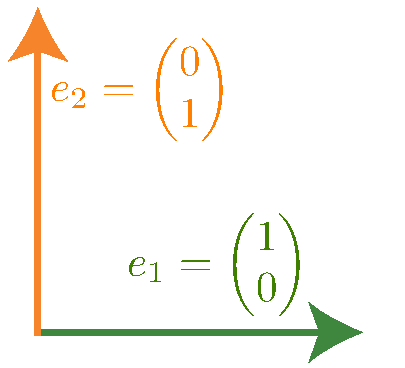
\includegraphics[scale=0.5]{Bilder/Abstand_bsp1.pdf}}} \qquad 
		\vcenter{\hbox{ $\begin{array}{rcl}
		\left\langle e_1 \mid e_2 \right\rangle & = & 0 \\
		\left\langle e_1 \mid e_1 \right\rangle & = & 1 \\
		\left\langle e_2 \mid e_2 \right\rangle & = & 1 \\
		e_1 \bot e_2 & &
	\end{array}$}}$ \\
$\vcenter{\hbox{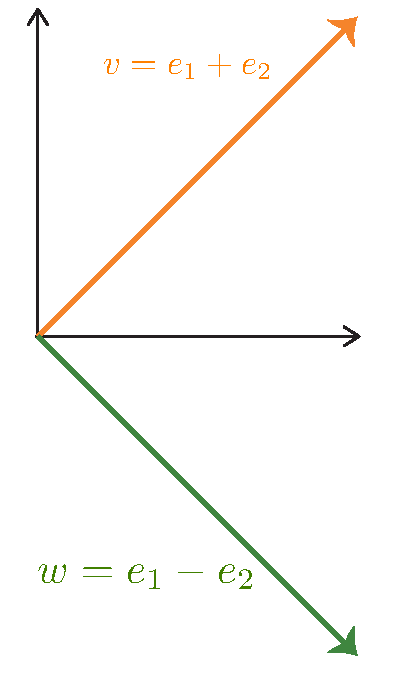
\includegraphics[scale=0.5]{Bilder/Abstand_bsp2.pdf}}} \qquad 
		\vcenter{\hbox{ $\begin{array}{rcl}
		\left\langle v \mid w \right\rangle & = & 0 \\
		\left\langle w \mid w \right\rangle & = & \left\langle e_1 - e_2 \mid e_1 -e_2 \right\rangle  \\
		& = & \left\langle e_1 \mid e_1 \right\rangle - \left\langle e_1 \mid e_2 \right\rangle + \left\langle e_2 \mid e_1 \right\rangle 
		+ \left\langle e_2 \mid e_2 \right\rangle \\
		& = & 2
	\end{array}$}}$ \\
$\vcenter{\hbox{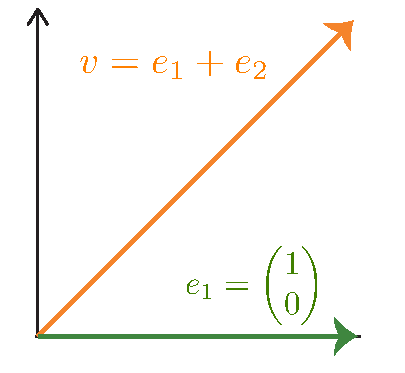
\includegraphics[scale=0.5]{Bilder/Abstand_bsp3.pdf}}} \qquad 
		\vcenter{\hbox{ $\begin{array}{rcl}
		\left\langle v \mid e_1 \right\rangle & = & \left\langle e_1 \mid e_1 \right\rangle + \left\langle e_2 \mid e_1 \right\rangle = 1 \\
		\left\langle v \mid v \right\rangle & = & 2 
	\end{array}$}}$ \\
$\vcenter{\hbox{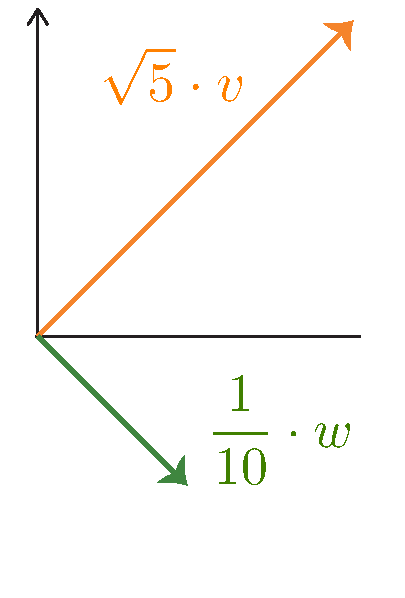
\includegraphics[scale=0.5]{Bilder/Abstand_bsp4.pdf}}} \qquad 
		\vcenter{\hbox{ $\begin{array}{rcl}
		\left\langle \sqrt{5} \cdot v  \mid \frac{1}{10} \cdot w  \right\rangle & = & \frac{\sqrt{5} }{10} \left\langle v \mid w \right\rangle  = 0\\
		\left\langle \sqrt{5} \cdot v  \mid \sqrt{5} \cdot v  \right\rangle & = & 5 \cdot 2 = 10 \\
		\left\langle \frac{1}{10} \cdot w  \mid \frac{1}{10} \cdot w  \right\rangle & = & \frac{1}{100} \cdot 2 = \frac{1}{50}   \\
	\end{array}$}}$
% subsection definition (end)

\subsection{Lemma} % (fold)
\label{sub:lemma}
Sind $v$ und $w$ orthogonal, so gilt 
\[
	|v+w|^2 = |v|^2 + |w|^2
\]
\underline{\textbf{Beweis:}} \\
\begin{align*}
	|v+w|^2 = \left\langle v+w \mid v+w \right\rangle = \left\langle v \mid v \right\rangle + \underbrace{\left\langle v \mid w \right\rangle +
	 \left\langle w \mid v \right\rangle}_{= 0 \text{ da } v \bot w}
	+ \left\langle w \mid w \right\rangle  = |v|^2 + |w|^2
\end{align*}
\hfill \( \square \)
% subsection lemma (end)

\subsection{Satz} % (fold)
\label{sub:satz}
Für $v,w \in V$ gilt 
\begin{enumerate}[(i)]
	\item $ \left| \left\langle v \mid w \right\rangle \right| \le |v| \cdot |w|$
	\item $|v+w| \le |v| + |w|$
\end{enumerate}
\underline{\textbf{Beweis:}} \\
\begin{enumerate}[(i)]
	\item Ist $v=0$ so ist $| \left\langle v \mid w \right\rangle | = 0 \le 0 = |v| |w|$. Sei also $v \not= 0$. Setze $\lambda  := 
	\frac{\left\langle v \mid w \right\rangle }{\left\langle v \mid v \right\rangle }$ ,  $w' := w - \overline{\lambda}  v$. Dann ist 
	\[
		\left\langle v \mid w' \right\rangle = \left\langle v \mid w \right\rangle - \left\langle v \mid \overline{\lambda}  v \right\rangle 
		= \left\langle v \mid w \right\rangle - \lambda \left\langle v \mid v \right\rangle = \left\langle v \mid w \right\rangle  - \left\langle v \mid w \right\rangle 
		= 0
	\]
	Also: $v \bot w'$. Also 
	\begin{align*}
		|w|^2 = | \overline{\lambda} v + w' |^2 \underset{\overline{\lambda} v \bot w' }{=} |\overline{\lambda}v|^2 + |w'|^2 &= |\lambda |^2  |v|^2 + |w'|^2 \\
		&\ge |\lambda|^2 |v|^2 \\
		&= \frac{| \left\langle v \mid w \right\rangle | ^2}{| \left\langle v \mid v \right\rangle |^2} |v|^2 \\
		&= \frac{|\left\langle v \mid w \right\rangle |^2}{\frac{|v|^4}{|v|^2} } = \frac{|\left\langle v \mid w \right\rangle |^2}{|v|^2}  
	\end{align*}
	Es folgt $|w|^2 |v|^2 \ge |\left\langle v \mid w \right\rangle |^2$ also auch $|w|\cdot |v| \ge | \left\langle v \mid w \right\rangle |$
	\item 
	\begin{align*}
		|v+w|^2 = \left\langle v+w \mid v+w \right\rangle &= \left\langle v \mid v \right\rangle + \left\langle w \mid v \right\rangle +
		 \left\langle v \mid w \right\rangle + \left\langle w \mid w \right\rangle  \\
		 &\le |v|^2 + |w|^2 + \underbrace{\left\langle w \mid v \right\rangle  + 
		 \overline{ \left\langle w \mid v \right\rangle } }_{2 |\left\langle v \mid w \right\rangle | \le 2 |v| |w|} \\
		 &\le |v|^2 + 2 |v| |w| + |w|^2 \\
		 &= (|v| + |w|)^2
	\end{align*}
	Es folgt
	\[
		|v+w| \le |v| + |w|
	\]
\end{enumerate}
% subsection satz (end)

\subsection{Definition} % (fold)
\label{sub:definition}
Sei $M \subseteq V \backslash \{0\}$. Dann heißt $M$ ein \underline{\textbf{Orthogonalsystem}}, wenn $\left\langle v \mid w \right\rangle = 0$ für alle $v,w \in M$ , 
$v \not= w$. Ein Orthogonalsystem aus Einheitsvektoren heißt ein \underline{\textbf{Orthonormalsystem}}. Eine Basis die auch ein Orhtonormalsystem ist, heißt eine \underline{\textbf{Orthonormalbasis}} (ONR).
% subsection definition (end)

\subsection{Lemma} % (fold)
\label{sub:lemma}
Sei $M$ ein Orthogonalsystem. Dann ist $M$ linear unabhängig.
\vspace{10pt} \\
\underline{\textbf{Beweis:}} \\
Seien $b_1, \ldots , b_n$ paarweise verschiedene Elemente von $M$ und $\lambda_1, \ldots , \lambda_n \in \mathds{K}$ mit 
\[
	\lambda_1 b_1 + \ldots + \lambda_n b_n = 0
\]
Für $i \in \{1, \ldots , n\}$ ist dann
\begin{align*}
	0= \left\langle \lambda_1 b_1 + \ldots + \lambda_n b_n \mid b_i \right\rangle &= \lambda_1 \underbrace{\left\langle b_1 \mid b_i \right\rangle}_{= 0} 
	+ \ldots + \lambda_i \left\langle b_i \mid b_i \right\rangle + \ldots + \lambda_n \underbrace{\left\langle b_n \mid b_i \right\rangle}_{=0} \\
	&= \lambda_i \underbrace{\left\langle b_i \mid b_i \right\rangle}_{\not= 0 \text{ da } b_i \not= 0}
\end{align*}
Also $\lambda_i = 0$ \hfill \( \square \)
% subsection lemma (end)

\subsection{Satz} % (fold)
\label{sub:satz}
Sei $M= \{ x_1, \ldots ,x_n \} \subseteq V$ linear unabhängig. Dann gibt es ein Orthogonalsystem $\{ e_1, \ldots , e_n \}$ sodass für alle $r \in \{1, \ldots ,n \}$ gilt:
\[
	\mathcal{L} ( e_1 , \ldots , e_r) = \mathcal{L} (x_1, \ldots , x_r)
\]
\underline{\textbf{Beweis:}} \\
Die Vektoren $e_1, \ldots , e_n$ werden induktiv definiert $e_1 := \frac{x_1}{|x_1|} $ ist ein Einheitsvektor. Sind $e_1, \ldots , e_r$ orthonormal, so ist der Vektor
$b_{r+1} := x_{r+1}- \sum\limits_{j=1}^{r} \left\langle x_{r+1} \mid e_j \right\rangle e_j $ orhtogonal zu $e_1, \ldots , e_r$. Ist $\mathcal{L} (e_1, \ldots , e_r)
= \mathcal{L} (x_1, \ldots , x_r)$, so ist $e_1, \ldots , e_r$ linear unabhängig und insbesondere $b_{r+1} \not= 0$. Nun setze
\[
	e_{r+1} := \frac{b_{r+1}}{|b_{r+1}|} 
\]
Dann ist $\{ e_1, \ldots , e_{r+1} \}$ ein Orthonormalsystem und es gilt
\[
	\mathcal{L} (e_1, \ldots , e_{r+1}) = \mathcal{L} (x_1, \ldots , x_{r+1})
\]
\hfill \( \square \)
% subsection satz (end)

\subsection{Korollar} % (fold)
\label{sub:korollar_14.9}
Ist $\dim V < \infty$, so besitzt $V$ eine Orthonormalbasis.
% subsection korollar_14.9 (end)

\subsection{Lemma} % (fold)
\label{sub:lemma_14.10}
Ist $e_1, \ldots , e_n$ eine Orthonormalbasis von $V$ gilt für jedes $v \in V$
\[
	v = \sum\limits_{j=1}^{n} \left\langle v \mid e_j \right\rangle  e_j 
\]
\underline{\textbf{Beweis:}} \\
Aus $v= \sum\limits_{j=1}^{n} \lambda_j e_j$ folgt
\[
	\left\langle v \mid e_{j_0} \right\rangle = \left\langle \sum\limits_{j=1}^{n} \lambda_j e_j \mid e_{j_0} \right\rangle 
	= \sum\limits_{j=1}^{n} \lambda_j \underbrace{\left\langle e_j \mid e_{j_0} \right\rangle}
	_{\substack{= 1 \text{ falls } j=j_0 \\ = 0 \text{ falls }j \not= j_0}}=\lambda_{j_0}
\]
\hfill \( \square \)
% subsection lemma_14.10 (end)

\subsection{Definition} % (fold)
\label{sub:definition_14.11}
Sei $U \le V$ ein Unterraum. Dann heißt
\[
	U^\bot := \Big\{ v \in V \mid v \bot u \text{ für alle } u \in U \Big\}
\]
das \underline{\textbf{orthogonale Komplement}} zu $U$.
% subsection definition_14.11 (end)

\subsection{Satz} % (fold)
\label{sub:satz_14.12}
Ist $\dim U < \infty$ so gilt $V=U \oplus U^\bot$.
\vspace{10pt} \\
\underline{\textbf{Beweis:}} \\
Ist $v \in U^\bot \cap U$ so gilt $\left\langle v \mid v \right\rangle = 0$, also $v=0$. Daher $U \cap U^\bot = \{0\}$. Sei $e_1, \ldots , e_n$ eine Orthonormalbasis von
$U$. Für $v \in V$ liegt dann 
\[
	W := v- \sum\limits_{j=1}^{n} \left\langle v \mid e_j \right\rangle e_j
\]
in $U^\bot$. Denn für $j_0 = 1, \ldots , n$ gilt:
\[
	\left\langle w \mid e_{j_0} \right\rangle = \left\langle v - \sum\limits_{j=1}^{n} \left\langle v \mid e_j \right\rangle e_j \mid e_{j_0} \right\rangle 
	= \left\langle v \mid e_{j_0} \right\rangle - \underbrace{\sum\limits_{j=1}^{n} \left\langle v \mid e_j \right\rangle \left\langle e_j \mid e_{j_0} \right\rangle }
	_{\left\langle v \mid e_{j_0} \right\rangle } = 0
\]
Also $e \bot e_j$ für $j= 1, \ldots , n$. Dann gilt auch $w \bot u$ für jedes $u = \sum\limits_{j=1}^{n} \lambda_j e_j \in U$. \\
(Denn: $\left\langle w \mid u \right\rangle = \left\langle w \mid \sum\limits_{j=1}^{n} \lambda_j e_j \right\rangle = \sum\limits_{j=1}^{n} \overline{\lambda_j}
\left\langle w \mid e_j \right\rangle = 0  $) \\
Also
\[
	v = \underset{\in U^\bot}{w} + \underbrace{\sum\limits_{j=1}^{n} \left\langle v \mid e_j \right\rangle e_j}_{\in U} \in U + U^\bot
\]
Damit gilt $V= U + U^\bot$
% subsection satz_14.12 (end)

\subsection{Definition} % (fold)
\label{sub:definition_14.13}
Eine \underline{\textbf{Projektion}} ist eine lineare Abbildung $p : V \to V$ mit $p \circ p = p$. Sie heißt \underline{\textbf{orthogonale Projektion}} auf $U$ falls
\[
	U = \text{Bild }p \quad , \quad U^\bot = \text{Kern }p
\]
\[
	\begin{tikzpicture}[scale=1.2]
	%\draw [help lines] (0,0) grid (6,3);
	\draw [blue, very thick](0,3) --(6,0);
	\node [below left] at (2,2) {$U$};
	\draw [orange,fill] (5,3) circle [radius= 0.05];
	\node [right] at (5,3) {$v$};
	\draw [dashed] (4,1) -- (5,3);
	\draw [thick,domain=63.434:153.434] plot ({cos(\x)* 0.7+4}, {sin(\x)* 0.7+1});
	\draw [fill] (3.92,1.35) circle [radius= 0.05];
	%\draw (4,1) circle [radius=0.5, start angle=30, end angle=120];
	\draw [fill] (4,1) circle [radius=0.05] node[below] (4,1) {$p(v)$};
\end{tikzpicture}
\]
% subsection definition_14.13 (end)

\subsection{Satz} % (fold)
\label{sub:satz_14.14}
Sei $U \le V$ , $\dim U < \infty$. Dann gilt: 
\begin{enumerate}[(i)]
	\item Es gibt genau eine orthogonale Projektion auf $U$
	\item Ist $p : V \to V$ die orthogonale Projektion auf $U$, so gilt für $u \in U, v \in V$ immer 
	\[
		|u-v| \ge | p(v)-v|
	\]
	Aus $|p(v)-v| = |u-v|$ folgt $u=p(v)$
\end{enumerate}
\underline{\textbf{Beweis:}} \\
\begin{enumerate}[(i)]
	\item Es ist $V= U \oplus U^\bot$. Also hat jeder Vektor $v \in V$ eine eindeutige Darstellung $v=u+ u'$ mit $u \in U, u' \in U^\bot$. Dann definiert
	$v \mapsto u$ eine orthogonale Projektion auf $U$. Ist $p : V \to V$ eine orthogonale Projektion auf $U$, so gilt 
	\[
		p(v)= p(u+u') = \underbrace{p(u)}_{\in U} + \underbrace{p(u')}_{\substack{= 0 \\ u' \in U^\bot = \ker p}}
	\]
	\item Es gilt
	\[
		|u-v|^2 = |p(u) - v|^2 = \Big| \underset{\in \text{ Bild }p = U}{\left(p(u) - p(v)\right)} + \underset{\in \ker p = U^\bot}{\left( p(v) - v \right)} \Big| ^2
		= |p(u) - p(v)|^2 + |p(v)-v|^2 \ge |p(v)-v|^2
	\]
	%\begin{align*}
		%|u-v|^2 = |p(u) - v|^2 = \Big| \underset{\in \text{ Bild }p &= U}{\left(p(u) - p(v)\right)} + \underset{\in \ker p \\
		%&= U^\bot}{\left( p(v) - v \right)} \Big| ^2 \\
		%&= |p(u) - p(v)|^2 + |p(v)-v|^2 \\
		%&\ge |p(v)-v|^2
	%\end{align*}
	Gilt $|u-v|=|p(v)-v|$ so folgt $|p(u) - p(v)| = 0$. Also $p(v)= p(u)= u$ \hfill \( \square \)
	\vspace{10pt} \\
	Hinweis:
	\[
		pv - v \in \ker p \text{ da } p(pv-v)= p(p(v))- p(v)=0
	\]
	
\end{enumerate}
% subsection satz_14.14 (end)

\subsection{Bemerkung} % (fold)
\label{sub:bemerkung_14.15}
Sei $B = e_1, \ldots , e_n$ eine Orthonormalbasis von $V$ und $f: V \to V$ linear. Dann gilt $m_B^B (f)= (a_{ij}) \in \mathds{K}^{n \times n}$ mit
$a_{ij}= \left\langle f(e_i) \mid e_j \right\rangle $, da 
\[
	f(e_i) = \sum\limits_{j=1}^{n} \left\langle f(e_i) \mid e_j \right\rangle e_j
\]
ist.
% subsection bemerkung (end)
% section euklidische_und_unitäre_vektorräume (end)

\section{Selbstadjungierte Endomorphismen} % (fold)
\label{sec:selbstadjungierte_endomorphismen}

\subsection{Definition} % (fold)
\label{sub:definition_15.1}
Sei $V$ ein euklididscher oder unitärer Vektorraum. Ein Endomorphismus heißt \underline{\textbf{selbstadjungiert}}, falls für alle $v,w \in V$ gilt
\[
	\left\langle f(v) \mid w \right\rangle = \left\langle v \mid f(w) \right\rangle 
\]
% subsection definition_15.1 (end)

\subsection{Lemma} % (fold)
\label{sub:lemma_15.2}
Sei $B=e_1, \ldots , e_n$ eine Orthonormalbasis von $V$. Dann ist $f : V \to V$ genau dann selbstadjungiert, wenn für $(a_{ij})= m_B^B (f)$ gilt 
$a_{ij} = \overline{a_{ji}} $
\vspace{10pt} \\
\underline{\textbf{Beweis:}} \\
Nach \ref{sub:bemerkung_14.15} ist $a_{ij}= \left\langle f(e_i) \mid e_j \right\rangle $. Ist $f$ selbstadjungiert, so folgt 
\[
	a_{ij} = \left\langle f(e_i) \mid e_j \right\rangle = \left\langle e_i \mid f(e_j) \right\rangle = \overline{\left\langle f(e_j) \mid e_i \right\rangle} = \overline{a_{ji}}   
\]
Ist umgekehrt $a_{ij} = \overline{a_{ji}} $ so folgt für $v,w \in V$ 
\begin{align*}
	\left\langle f(v) \mid w \right\rangle = \left\langle f\left(\sum\limits_{i=1}^{n} \left\langle v \mid e_i \right\rangle  e_i \right) \mid 
	\sum\limits_{j=1}^{n} \left\langle w \mid e_j \right\rangle e_j \right\rangle &= \sum\limits_{i=1}^{n} \sum\limits_{j=1}^{n} \left\langle v \mid e_i \right\rangle 
	\overline{\left\langle w \mid e_j \right\rangle} \underbrace{\left\langle f(e_i) \mid e_j \right\rangle}_{= a_{ij} = \overline{a_{ji}} =
	\overline{\left\langle f(e_j) \mid e_i \right\rangle } = \left\langle e_i \mid f(e_j) \right\rangle   } \\
	&= \sum\limits_{i=1}^{n} \sum\limits_{j=1}^{n} \left\langle v \mid e_i \right\rangle \overline{\left\langle w \mid e_j \right\rangle } \left\langle e_i \mid f(e_j) \right\rangle  \\
	&= \left\langle \underbrace{\sum\limits_{i=1}^{n} \left\langle v \mid e_i \right\rangle e_i}_{v} \, \Bigg| \,
	 f \underbrace{ \left( \sum\limits_{j=1}^{n} \left\langle w \mid e_j \right\rangle e_j \right)}_{w} \right\rangle \\
	&= \left\langle v \mid f(w) \right\rangle 
\end{align*}
% subsection lemma_15.2 (end)

\subsection{Beispiel} % (fold)
\label{sub:beispiel_15.3}
\begin{enumerate}[(i)]
	\item Sei $A= (a_{ij}) \in \mathds{R}^{n \times n}$. Dann ist 
	\[
		f_A : \mathds{R}^n \to \mathds{R}^n \enspace , \enspace v \mapsto Av
	\]
	genau dann selbstadjungiert (bzgl. dem Standardskalarprodukt auf dem $\mathds{R}^n$) wenn 
	\[
		A = A^t
	\]
	In diesem Fall heißt $A$ \underline{\textbf{symmetrisch}}.
	\item Sei $A= (a_{ij}) \in \mathds{C}^{n \times n}$. Dann ist 
	\[
		f_A : \mathds{C}^n \to \mathds{C}^n \enspace , \enspace v \mapsto Av
	\]
	genau dann selbstadjungiert (bzgl. dem Standardskalarprodukt auf dem $\mathds{C}^n$) wenn 
	\[
		A = \overline{A}^t \quad \text{also für } A = (a_{ij}) \enspace (a_{ij}) =  \overline{a_{ji}} \text{ gilt}
	\]
	In diesem Fall heißt $A$ \underline{\textbf{hermitesch}}.
\end{enumerate}
% subsection beispiel_15.3 (end)

\subsection{Lemma} % (fold)
\label{sub:lemma}
Sei $f : V \to V$ selbstadjungiert. Dann gilt:
\begin{enumerate}[(i)]
	\item Alle Eigenwerte sind reell
	\item Eigenvektoren zu verschiedenen Eigenwerten sind orthogonal
	\item Ist $U \le V$ ein Unterraum mit $f(U) \subseteq U$, so gilt auch $f(U^\bot) \subseteq U^\bot$
\end{enumerate}
\underline{\textbf{Beweis:}}
\begin{enumerate}[(i)]
	\item Sei $\lambda \in \mathds{C}$ ein Eigenwert. Dann gibt es $v \not= 0 \in V$ mit $f(v)= \lambda v$ ($v$ ist Eigenvektor zu $\lambda$). Dann ist 
	\[
		\lambda \left\langle v \mid v \right\rangle = \left\langle \lambda v \mid v \right\rangle = \left\langle f(v) \mid v \right\rangle = \left\langle v \mid f(v)
		\right\rangle = \left\langle v \mid \lambda v \right\rangle = \overline{\lambda} \left\langle v \mid v \right\rangle  
	\]
	Da mit $v \not= 0$ auch $\left\langle v \mid v \right\rangle \not= 0$ ist, folgt $\lambda = \overline{\lambda} $. Also ist $\lambda $ reell.
	\item Seien $f(v)=\lambda v$ , $f(w)= \mu w$ mit $v,w \in V, \lambda \not= \mu \in \mathds{K}$. Es folgt
	\[
		\lambda \left\langle v \mid w \right\rangle = \left\langle \lambda v \mid w \right\rangle = \left\langle f(v) \mid w \right\rangle = 
		\left\langle v \mid f(w) \right\rangle = \left\langle v \mid \mu w \right\rangle = \overline{\mu} \left\langle v \mid w \right\rangle  = 
		\mu \left\langle v \mid w \right\rangle 
	\]
	Also $(\lambda - \mu) \left\langle v \mid w \right\rangle = 0$ $\overset{\lambda \not= \mu}{\Longrightarrow} \left\langle v \mid w \right\rangle = 0$
	\item Sei $v \in U^\bot$. Zu zeigen: $\forall u \in U$ gilt $\left\langle f(v) \mid u \right\rangle = 0$
	\[
		\left\langle f(v) \mid u \right\rangle = \left\langle \underset{\in U^\bot}{v} \mid \underset{\in U}{f(u)} \right\rangle  = 0
	\]
	\hfill \( \square \)
\end{enumerate}
% subsection lemma (end)

\subsection{Satz} % (fold)
\label{sub:satz}
Jeder selbstadjungierte Endomorphismus eines endlich dimensionalen euklidischen oder unitären Vektorraumes ist diagonalisierbar.
\vspace{10pt} \\
\underline{\textbf{Beweis:}} für $\mathds{K} = \mathds{C}$\\
Zu zeigen: $\exists$ Basis aus Eigenvektoren.  \\
Induktion nach $n := \dim V$ \\
\textbf{Induktionsanfang:} $n=0 \surd$ \\
\textbf{Induktionsschritt:} $n-1 \mapsto n$ \\
Nach dem Fudamentalsatz der Algebra ($\mathds{K}=\mathds{C}$ !) hat $\chi_f$ eine Nullstelle $\lambda \in \mathds{C}$. Also ist $\lambda $ ein Eigenwert von $f$.
Sei $v \in V$ ein zugehöriger Eigenvektor. Sei $U:= \mathcal{L} (v)^\bot = \{ \mu \cdot c \mid \mu \in \mathds{C}\}^\bot$. Dann 
\[
	V = \mathcal{L} \big( \{v\} \big) \oplus U
\]
also $\dim U = \dim V - \dim \mathcal{L} \big( \{v\} \big) = n-1$. Da 
\[
	f \Big(\mathcal{L} \big(\{v\} \big)\Big)= \mathcal{L} \big( \{f(v)\} \big) 
	= \mathcal{L} \big( \{ \lambda \cdot v\} \big) \subseteq  \mathcal{L} \big( \{\cdot v\} \big)
\]
folgt mit 15.4 (iii) $f(U) \subseteq U$. also ist $f \big|_U : U \to U$ ein selbstadjungierter Endomorphismus von $U$. \\
Induktionsannahme $\Rightarrow f \big|_U$ ist diagonalisierbar, also gibt es eine Basis  von $U$ $b_1, \ldots , b_{n-1}$ aus Eigenvektoren von $f$. 
Nun ist $v, b_1, \ldots , b_{n-1}$ eine Basis aus Eigenvektoren für $f$ \hfill \( \square \) 
% subsection satz (end)

\subsection{Korollar} % (fold)
\label{sub:korollar}
Symmetrische und hermitesche Matrizen sind diagonalisierbar. (Dabei sind alle Eigenwerte reell)
\vspace{\baselineskip} \\
\underline{\textbf{Beweis (15.6):}} \\
Folgt aus 15.5 , 15.3 , 15.4 \hfill \( \square \)
% subsection korollar (end)

\subsection{Lemma} % (fold)
\label{sub:lemma}
Sei $f : V \to V$ selbstadjungiert, wobei $V$ ein euklidischer endlich dimensionaler Vektorraum ist. Dann besitzt $f$ einen Eigenwert
\vspace{10pt} \\
\underline{\textbf{Beweis:}} \\
Sei $B$ eine Basis Orthonormalbasis von $V$ ($\dim V = n$). Sei $A= m_B^B (f) \in \mathds{R}^{n \times n}$. Da $f$ selbstadjungiert ist (und $B$ eine ONB), ist
$A$ symetrisch, also $A= A^t$. Nun ist $f_A : \mathds{C}^n \to \mathds{C}^n$ ein selbstadjungierter Endomorphismus von $\mathds{C}^n$ und besitzt einen reellen 
Eigenwert $\lambda$. \\
Da $\chi_f = \chi_A = \chi_{f_A}$ ist $\lambda$ eine Nullstelle von $\chi_{f_A}=\chi_f$ also auch ein Eigenwert von $f$. \hfill \( \square \)
% subsection lemma (end)
% section selbstadjungierte_endomorphismen (end)


\cleardoubleoddemptypage
\pagenumbering{Alph}
\setcounter{page}{1}
\printindex
\listoffigures
\end{document}